% =====================================================================
%  FUSE-Based File System with Custom Disk Scheduling and Synchronization
%  (implementation name: SchedFS)
%  Operating Systems Lab (24B11CS312) -- Project Report
%  Formatting follows the approved project synopsis.
%  Compile: pdflatex -> bibtex -> pdflatex -> pdflatex   (or run build.sh)
% =====================================================================
\documentclass[12pt,a4paper]{article}

% ---------------------------------------------------------------------
%  Course details (from the approved synopsis)
% ---------------------------------------------------------------------
\newcommand{\coursename}{Operating Systems Lab}
\newcommand{\coursecode}{24B11CS312}
\newcommand{\projecttitle}{FUSE-Based File System with Custom Disk Scheduling and Synchronization}

% ---------------------------------------------------------------------
%  Fonts, page geometry and layout (matched to the synopsis)
% ---------------------------------------------------------------------
\usepackage[T1]{fontenc}
\usepackage[utf8]{inputenc}
\usepackage{lmodern}
\usepackage[a4paper,margin=1in,footskip=0.42in]{geometry}
\usepackage{setspace}
\setstretch{1.345}  % 19.5 pt between baselines of 12 pt text, as in the synopsis
\usepackage{etoolbox}
\usepackage{microtype}
\DisableLigatures[-]{encoding=T1, family=tt*}
\usepackage{graphicx}
\usepackage{float}
\usepackage{booktabs}
\usepackage{longtable}
\usepackage{array}
\usepackage{tabularx}
\usepackage{multirow}
\usepackage{makecell}
\usepackage[font={small,stretch=1.0},labelfont=bf,labelsep=quad,justification=centering]{caption}
\usepackage{subcaption}
\usepackage{tikz}
\usetikzlibrary{arrows.meta,positioning,shapes.geometric,shapes.misc,fit,calc,backgrounds,decorations.pathreplacing}
\usepackage{pgfplots}
\usepgfplotslibrary{groupplots}
\pgfplotsset{compat=1.18}
\usepackage{listings}
\usepackage{xcolor}
\usepackage{amsmath}
\usepackage{enumitem}
\usepackage{eso-pic}
\usepackage{titlesec}
\usepackage{tocloft}
\usepackage{needspace}
\usepackage{cite}
\usepackage[hidelinks]{hyperref}

\setlength{\emergencystretch}{2.5em}
\setlength{\parindent}{1.5em}
\setlength{\parskip}{0pt}
\renewcommand{\arraystretch}{1.18}
\setlist{itemsep=2pt,topsep=4pt}
\captionsetup[table]{position=top,skip=5pt}
\captionsetup[figure]{name=Fig.,skip=6pt}
\captionsetup[lstlisting]{font={small,stretch=1.0},labelfont=bf,labelsep=quad,skip=4pt}

% Tables, diagrams, listings and lists of contents use single spacing, as in the synopsis
\AtBeginEnvironment{tabular}{\setstretch{1.0}}
\AtBeginEnvironment{tabularx}{\setstretch{1.0}}
\AtBeginEnvironment{longtable}{\setstretch{1.0}}
\AtBeginEnvironment{tikzpicture}{\setstretch{1.0}}

% Page border on every page, as in the synopsis (0.6 pt)
\AddToShipoutPictureBG{\AtPageLowerLeft{%
  \begin{tikzpicture}
    \path (0,0);
    \draw[line width=0.6pt] (33.7bp,33.7bp) rectangle (561.6bp,808.0bp);
  \end{tikzpicture}}}

% Left-aligned headings: 16 pt bold sections, 14 pt bold subsections (synopsis style)
\titleformat{\section}{\fontsize{15.9}{19}\selectfont\bfseries}{\thesection.}{0.55em}{}
\titlespacing*{\section}{0pt}{20pt plus 4pt minus 2pt}{10pt plus 2pt}
\titleformat{\subsection}{\fontsize{13.9}{17}\selectfont\bfseries}{\thesubsection}{1em}{}
\titlespacing*{\subsection}{0pt}{14pt plus 3pt minus 2pt}{6pt plus 1pt}
\titleformat{\subsubsection}{\normalsize\bfseries}{\thesubsubsection}{0.8em}{}
\titlespacing*{\subsubsection}{0pt}{10pt plus 2pt minus 1pt}{4pt}
\setcounter{secnumdepth}{3}
\setcounter{tocdepth}{2}
\renewcommand{\cftsecleader}{\cftdotfill{\cftdotsep}}
\renewcommand{\cftsecaftersnum}{.}
\setlength{\cftbeforesecskip}{6pt}
\renewcommand{\contentsname}{Table of Contents}
\renewcommand{\listfigurename}{List of Figures}
\renewcommand{\listtablename}{List of Tables}
\renewcommand{\cftfigpresnum}{Fig.~}
\setlength{\cftfignumwidth}{3.6em}
\renewcommand{\cfttabpresnum}{Table~}
\setlength{\cfttabnumwidth}{4.2em}

% ---------------------------------------------------------------------
%  Code listings
% ---------------------------------------------------------------------
\definecolor{kw}{RGB}{20,60,140}
\definecolor{cm}{RGB}{60,110,60}
\definecolor{st}{RGB}{150,40,40}
\definecolor{ln}{RGB}{140,140,140}
\lstdefinestyle{cstyle}{
  language=C,
  basicstyle=\ttfamily\footnotesize,
  keywordstyle=\color{kw},
  commentstyle=\color{cm}\itshape,
  stringstyle=\color{st},
  numbers=left, numberstyle=\tiny\color{ln}, numbersep=7pt,
  xleftmargin=2.2em, framexleftmargin=1.6em,
  frame=tb, framerule=0.4pt, framesep=3pt,
  breaklines=true, breakatwhitespace=false, postbreak=\mbox{$\hookrightarrow$\space},
  columns=fullflexible, keepspaces=true, tabsize=4,
  showstringspaces=false, captionpos=t, upquote=true,
  morekeywords={uint8_t,uint16_t,uint32_t,uint64_t,size_t,ssize_t,off_t,mode_t,bool,true,false,
    pthread_mutex_t,pthread_cond_t,pthread_t,disk_request_t,request_queue_t,scheduler_t,
    sfs_t,sfs_inode_t,sfs_superblock_t,sfs_dirent_t,virtual_disk_t,sched_policy_t,_Static_assert}
}
\lstdefinestyle{shstyle}{
  language=bash, basicstyle=\ttfamily\footnotesize, keywordstyle=\color{kw},
  commentstyle=\color{cm}\itshape, stringstyle=\color{st},
  numbers=left, numberstyle=\tiny\color{ln}, numbersep=7pt,
  xleftmargin=2.2em, framexleftmargin=1.6em, frame=tb, framerule=0.4pt,
  breaklines=true, columns=fullflexible, keepspaces=true, showstringspaces=false, upquote=true
}
\lstset{style=cstyle}
% keep each listing's caption on the same page as its first lines of code
\let\origlstinputlisting\lstinputlisting
\renewcommand{\lstinputlisting}[2][]{\needspace{8\baselineskip}\begingroup\setstretch{1.0}\origlstinputlisting[#1]{#2}\endgroup}
\AtBeginEnvironment{lstlisting}{\setstretch{1.0}}
\renewcommand{\lstlistingname}{Listing}
\renewcommand{\lstlistlistingname}{List of Listings}

% ---------------------------------------------------------------------
%  Diagram styles
% ---------------------------------------------------------------------
\tikzset{
  >={Stealth[length=2.2mm]},
  box/.style={draw, rounded corners=2pt, fill=gray!7, align=center, font=\small,
              text width=#1, minimum height=0.85cm, inner sep=3pt},
  box/.default=2.8cm,
  hbox/.style={box=#1, fill=blue!7, draw=blue!45!black},
  hbox/.default=2.8cm,
  proc/.style={draw, rounded corners=1.5pt, fill=white, align=center, font=\footnotesize,
               text width=#1, minimum height=0.7cm, inner sep=2.5pt},
  proc/.default=3.4cm,
  dec/.style={draw, diamond, aspect=2.3, fill=gray!7, align=center, font=\footnotesize,
              inner sep=0.5pt, text width=#1},
  dec/.default=2.4cm,
  term/.style={draw, rounded rectangle, fill=gray!18, align=center, font=\footnotesize\bfseries,
               minimum height=0.65cm, inner xsep=8pt},
  io/.style={draw, trapezium, trapezium left angle=72, trapezium right angle=108, fill=white,
             align=center, font=\footnotesize, text width=#1, minimum height=0.65cm, inner sep=2pt},
  io/.default=3cm,
  arr/.style={->, semithick},
  lab/.style={font=\scriptsize, fill=white, inner sep=1pt},
  note/.style={font=\scriptsize\itshape, align=left, text=black!75},
  store/.style={draw, cylinder, shape border rotate=90, aspect=0.22, fill=gray!12,
                minimum width=2.4cm, minimum height=1.05cm, align=center, font=\small},
}

\DeclareRobustCommand{\code}[1]{\texttt{\detokenize{#1}}}
\newcommand{\figref}[1]{Fig.~\ref{#1}}
\newcommand{\tabref}[1]{Table~\ref{#1}}

\begin{document}

% =====================================================================
%  TITLE PAGE  (layout reproduced from the approved synopsis;
%  "PROJECT SYNOPSIS" becomes "PROJECT REPORT")
% =====================================================================
\begin{titlepage}
\thispagestyle{empty}
\begin{tikzpicture}[remember picture,overlay,
    every node/.style={inner sep=0pt, outer sep=0pt}]
  \coordinate (O) at (current page.north west);
  \def\cx{297.6bp}
  \node[anchor=north] at ($(O)+(\cx,-70bp)$) {\fontsize{17.9}{21}\selectfont\bfseries PROJECT REPORT};
  \node[anchor=north] at ($(O)+(\cx,-102bp)$) {\fontsize{15.9}{19}\selectfont on};
  \node[anchor=north] at ($(O)+(\cx,-135bp)$) {\fontsize{17.9}{21}\selectfont\bfseries FUSE-BASED FILE SYSTEM WITH CUSTOM};
  \node[anchor=north] at ($(O)+(\cx,-166bp)$) {\fontsize{17.9}{21}\selectfont\bfseries DISK SCHEDULING AND};
  \node[anchor=north] at ($(O)+(\cx,-197bp)$) {\fontsize{17.9}{21}\selectfont\bfseries SYNCHRONIZATION};
  \node[anchor=north] at ($(O)+(\cx,-265.8bp)$) {
\includegraphics[width=101.5bp]{figures/jiit_logo_0.png}};
  \node[anchor=north] at ($(O)+(\cx,-455bp)$) {\bfseries \coursename{} (\coursecode)};
  \node[anchor=north] at ($(O)+(\cx,-474bp)$) {Project Based Learning (PBL)};
  \node[anchor=north] at ($(O)+(\cx,-493bp)$) {Odd Semester 2026, Academic Session 2026--27};
  \node[anchor=north west] at ($(O)+(72bp,-566bp)$) {\bfseries SUBMITTED TO};
  \node[anchor=north west] at ($(O)+(72bp,-591bp)$) {Dr. Tanvi Gautam};
  \node[anchor=north west] at ($(O)+(72bp,-613bp)$) {Dr. Sayani Ghosal};
  \node[anchor=north west] at ($(O)+(72bp,-634bp)$) {Mr. Umar Farooq};
  \node[anchor=north west] at ($(O)+(345bp,-566bp)$) {\bfseries SUBMITTED BY};
  \node[anchor=north west] at ($(O)+(345bp,-591bp)$) {Saanvi Grover};
  \node[anchor=north west] at ($(O)+(465bp,-591bp)$) {2408030010};
  \node[anchor=north west] at ($(O)+(345bp,-613bp)$) {Prankit Goel};
  \node[anchor=north west] at ($(O)+(465bp,-613bp)$) {2408030011};
  \node[anchor=north west] at ($(O)+(345bp,-634bp)$) {Aditya Sharma};
  \node[anchor=north west] at ($(O)+(465bp,-634bp)$) {2408030019};
  \node[anchor=north west] at ($(O)+(345bp,-655bp)$) {Aaradhya Kulashri};
  \node[anchor=north west] at ($(O)+(465bp,-655bp)$) {2408030026};
  \node[anchor=north] at ($(O)+(\cx,-725bp)$) {\fontsize{11.5}{14}\selectfont\bfseries DEPARTMENT OF COMPUTER SCIENCE ENGINEERING};
  \node[anchor=north] at ($(O)+(\cx,-743bp)$) {\fontsize{11.5}{14}\selectfont\bfseries JAYPEE INSTITUTE OF INFORMATION TECHNOLOGY,};
  \node[anchor=north] at ($(O)+(\cx,-761bp)$) {\fontsize{11.5}{14}\selectfont\bfseries NOIDA (U.P.) NOVEMBER 2026};
\end{tikzpicture}
\end{titlepage}

% =====================================================================
%  FRONT MATTER
% =====================================================================
\pagenumbering{roman}
\setcounter{page}{2}  % the title page counts as page i, as in the synopsis
\tableofcontents
\clearpage
\listoffigures
\clearpage
\listoftables
\vspace{1.2em}
\lstlistoflistings
\clearpage
\pagenumbering{arabic}
\setcounter{page}{1}

% =====================================================================
\section{TITLE OF THE PROJECT}
\label{sec:title}
% =====================================================================
\begin{center}
\fontsize{13.9}{18}\selectfont\bfseries \projecttitle
\end{center}

\noindent This is the title approved in the project synopsis. The implementation is called \textbf{SchedFS}: a mountable Linux file system written in C11 on the FUSE~3 interface. Every block that the file system reads or writes is turned into a request, queued, and served in the order chosen by a disk-scheduling policy (FCFS, SSTF, SCAN or Adaptive) that is selected when the file system is mounted. The project therefore joins two chapters of an operating-systems course---\emph{file systems} and \emph{disk scheduling}---and adds a third, \emph{process synchronization}, because the queue between them is a bounded producer--consumer buffer shared by several threads.

\begin{table}[H]
\centering
\caption{Project identification}
\label{tab:ident}
\small
\begin{tabularx}{\linewidth}{@{}>{\bfseries}p{3.6cm}X@{}}
\toprule
Project title & \projecttitle \\
Implementation & SchedFS (repository name \code{FUSE}) \\
Course & \coursename{} (\coursecode), Project Based Learning \\
Session & Odd Semester 2026, Academic Session 2026--27 \\
Supervisors & Dr. Tanvi Gautam, Dr. Sayani Ghosal, Mr. Umar Farooq \\
Category & Systems programming: file systems, disk scheduling, synchronization \\
Platform & Linux (Ubuntu 22.04/24.04), FUSE~3, GNU C11, POSIX threads \\
Source repository & \url{https://github.com/Sharmaditya2k05/FUSE} \\
Interactive demo & \url{https://sharmaditya2k05.github.io/FUSE/} \\
\bottomrule
\end{tabularx}
\end{table}

% =====================================================================
\section{ABSTRACT OF THE PROJECT}
\label{sec:abstract}
% =====================================================================
Operating-systems courses treat file systems and disk scheduling as separate topics, so students rarely see a scheduling policy act on the I/O stream of a real file system. SchedFS joins the two. It is a mountable Linux file system implemented in C11 on the FUSE~3 interface. Its data lives in a single image file with a superblock, a free-block bitmap, 256 fixed-size inodes and 4~KiB data blocks reached through direct and single-indirect pointers. Every block read or write issued by the file system becomes a request in a bounded producer--consumer queue protected by a mutex and two condition variables. A single dispatcher thread selects the next request with a policy chosen at mount time---first-come first-served (FCFS), shortest seek time first (SSTF), SCAN, or an age-aware Adaptive policy---and only then calls \code{pread} or \code{pwrite} on the image, while each caller sleeps on its own condition variable until its request completes. The system also records seek distance and waiting time, and includes a trace-replay benchmark and a web visualisation. On the classic textbook trace the scheduler reproduces head movements of 640, 236 and 236 blocks for FCFS, SSTF and SCAN. On the mounted file system with four concurrent writers, SSTF reduced total head movement by 40\,\% compared with FCFS. Scheduler unit tests, core concurrency tests and mounted FUSE system tests all pass, and ThreadSanitizer reports no data races.

% =====================================================================
\section{SCOPE OF THE PROJECT}
\label{sec:scope}
% =====================================================================
\textbf{Problem and objectives.} Disk-scheduling algorithms are normally studied on hand-written request lists \cite{silberschatz2018,tanenbaum2015}, detached from the software that produces disk traffic. The objective of SchedFS is to place these algorithms inside a working file system, so that ordinary commands such as \code{cp}, \code{cat} and \code{mkdir} generate the requests and the effect of each policy can be observed and measured. A second objective is to show correct multi-threaded synchronization: many FUSE worker threads produce requests concurrently, and a single consumer must serve them without races, lost wake-ups or deadlock.

\textbf{Scope and boundaries.} SchedFS implements an on-disk format, a formatter (\code{mkfs.schedfs}), the core file operations (create, read, write, truncate, rename, unlink, mkdir, rmdir, readdir, stat and statfs), four scheduling policies, metric collection, a benchmark harness and a test suite. Seek distance is modelled as the absolute difference between block numbers, as in textbook disk scheduling; the image file itself is stored on whatever device hosts it, so the project measures scheduling decisions rather than physical seek time. Journaling, crash recovery, hard and symbolic links, extended attributes, ACL enforcement and a block cache are outside the scope.

\textbf{Intended users.} The primary users are operating-systems students and instructors who want to see scheduling and synchronization at work on real I/O. The benchmark and the web visualisation also serve as teaching aids during lectures and viva examinations.

\textbf{Operating-systems relevance.} The project exercises file-system layout and indexed allocation, free-space management with a bitmap, disk scheduling, the bounded-buffer problem, mutexes, condition variables and reader--writer locks, lock ordering for deadlock avoidance, user-space file systems and the system-call interface (\code{open}, \code{pread}, \code{pwrite}, \code{fsync}, \code{fork} during daemonization) \cite{silberschatz2018,arpaci2018,kerrisk2010}.

\textbf{Practical applications.} The same layering---a request queue in front of a block device with a pluggable policy---is used by real I/O schedulers in operating-system kernels \cite{worthington1994}. SchedFS can be used to compare policies on custom workloads, to demonstrate starvation and fairness, and as a starting point for adding policies such as C-SCAN or LOOK.

\textbf{Limitations.} The maximum file size is 1{,}036 blocks (about 4.05~MiB). A clean unmount is required for persistence because there is no journal. \code{rename} refuses to replace an existing target. The image format is native little-endian and intended for Linux on x86-64.

% ---------------------------------------------------------------------
\renewcommand{\thesubsection}{\thesection(\alph{subsection})}
\subsection{Functional Requirements}
\label{sec:fr}
% ---------------------------------------------------------------------
\tabref{tab:fr} lists twelve functional requirements, against the minimum of eight ($2 \times 4$). Each one is implemented and is exercised by a test or a captured run in Section~\ref{sec:testing}.

{\small
\begin{longtable}{@{}p{0.9cm}p{3.1cm}p{7.3cm}p{2.6cm}@{}}
\caption{Functional requirements}\label{tab:fr}\\
\toprule
\textbf{ID} & \textbf{Requirement} & \textbf{Description and expected functionality} & \textbf{Module} \\
\midrule
\endfirsthead
\toprule
\textbf{ID} & \textbf{Requirement} & \textbf{Description and expected functionality} & \textbf{Module} \\
\midrule
\endhead
\bottomrule
\endfoot
FR1 & Format an image & \code{mkfs.schedfs IMAGE SIZE} creates a new image, writes the superblock, bitmap, inode table and root directory, and refuses to overwrite an existing file or accept an invalid size. & M1 Formatter \\
FR2 & Mount as a Linux file system & \code{schedfs IMAGE MOUNTPOINT --sched=POLICY} validates the image, prints its geometry and mounts it through FUSE, in the foreground (\code{-f}) or as a background daemon. & M2 FUSE adapter \\
FR3 & Create, read and write files & Regular files can be created, written at any offset and read back byte-for-byte, including files larger than 48~KiB that need the single-indirect block. & M3, M4 \\
FR4 & Directory operations & \code{mkdir}, \code{rmdir} and \code{readdir} work on nested directories; removing a non-empty directory fails with \code{ENOTEMPTY}. & M3 Inode and directory layer \\
FR5 & Rename, delete and truncate & \code{rename}, \code{unlink} and \code{truncate} are supported; truncating to a larger size creates a sparse region that reads as zeros. & M3, M4 \\
FR6 & Metadata and capacity & \code{stat} reports size, mode, owner and timestamps; \code{df} reports total and free capacity through \code{statfs}. & M2, M3 \\
FR7 & Scheduled block I/O & Every block read or write after mounting is submitted as a request to a bounded queue and performed only by the dispatcher thread. & M5, M7 \\
FR8 & Selectable scheduling policies & FCFS, SSTF, SCAN and Adaptive are selectable at mount time; Adaptive is tunable with \code{--alpha} and \code{--beta}. Invalid policy names or negative weights are rejected. & M6 Scheduler \\
FR9 & Persistence & Data and metadata written before a clean unmount are present after remounting, including under a different policy. & M3, M7 \\
FR10 & Metrics and logging & Request count and total seek distance are logged at unmount; \code{--verbose} adds DEBUG entries such as block allocations to \code{filesystem.log}. & M8 Metrics and logging \\
FR11 & Benchmark and graphs & \code{schedfs-bench --all} replays five fixed traces under every policy and writes \code{benchmark.csv}; \code{plot\_results.py} draws comparison graphs. & M9 Benchmark \\
FR12 & Interactive visualisation & A web page animates the head movement of each policy on the textbook and benchmark traces using a port of \code{scheduler\_pick()}. & M9 Benchmark and visualisation \\
\end{longtable}
}

% ---------------------------------------------------------------------
\subsection{Non-Functional Requirements}
\label{sec:nfr}
% ---------------------------------------------------------------------
\tabref{tab:nfr} lists eight non-functional requirements, against the minimum of four ($1 \times 4$), each with the criterion used to check it.

{\small
\begin{longtable}{@{}p{0.9cm}p{2.6cm}p{6.6cm}p{3.8cm}@{}}
\caption{Non-functional requirements}\label{tab:nfr}\\
\toprule
\textbf{ID} & \textbf{Quality} & \textbf{How it applies to SchedFS} & \textbf{Measurable criterion} \\
\midrule
\endfirsthead
\toprule
\textbf{ID} & \textbf{Quality} & \textbf{How it applies to SchedFS} & \textbf{Measurable criterion} \\
\midrule
\endhead
\bottomrule
\endfoot
NFR1 & Correctness and reliability & Data written through the mount must read back identically and survive remounting. & \code{cmp} reports identical files; all \code{make test} stages pass (Section~\ref{sec:results}). \\
NFR2 & Thread safety & Concurrent FUSE worker threads share the queue, bitmap, inode table and superblock. & ThreadSanitizer reports no data race in the 4-thread core test. \\
NFR3 & Deadlock freedom & Locks are always acquired in one documented global order. & No hang in any test run; lock order in \figref{fig:locks}. \\
NFR4 & Determinism & The same request set must give the same service order for a policy. & Ties broken by arrival time, then request ID; FCFS, SSTF and SCAN seek totals are identical across runs. \\
NFR5 & Bounded resource use & The queue holds at most 128 requests; metadata overhead is fixed. & Queue capacity 128; metadata uses 10 of 4{,}096 blocks (0.24\,\%) on a 16~MiB image. \\
NFR6 & Maintainability & Code is split into layered modules with small interfaces and a fixed style. & 8 headers, one module per directory, \code{clang-format} style; builds with \code{-Wall -Wextra -Wpedantic -Wshadow -Wconversion} and no warnings. \\
NFR7 & Usability & Commands follow normal Linux conventions and give clear error messages. & Usage text on invalid options; standard \code{errno} messages (\figref{fig:term-errors}, \figref{fig:term-ops}). \\
NFR8 & Portability & Runs on any Linux system with libfuse~3 and a C11 compiler. & Built and tested on Ubuntu 24.04 with GCC 13.3 and libfuse 3.14. \\
\end{longtable}
}

% ---------------------------------------------------------------------
\subsection{Description of the Modules of the Project}
\label{sec:modules}
% ---------------------------------------------------------------------
SchedFS is organised into ten modules, against the minimum of eight ($2 \times 4$). Nine follow directly from the source tree. The inode and directory layer (M3) and the block-allocation and mapping layer (M4) share \code{src/fs/filesystem.c}, but they are separate groups of functions with separate locks, so they are described separately. \tabref{tab:modsummary} gives an overview, and the paragraphs that follow describe each module.

\begin{table}[H]
\centering
\caption{Module overview}
\label{tab:modsummary}
\small
\begin{tabularx}{\linewidth}{@{}l l X r@{}}
\toprule
\textbf{ID} & \textbf{Module} & \textbf{Main source files} & \textbf{LOC} \\
\midrule
M1 & Image formatter & \code{mkfs/mkfs.c}, \code{include/layout.h} & 180 \\
M2 & FUSE adapter & \code{src/fuse/fuse_main.c} & 199 \\
M3 & Inode and directory layer & \code{src/fs/filesystem.c} (paths, inodes, dirs) & \multirow{2}{*}{808} \\
M4 & Block allocation and mapping & \code{src/fs/filesystem.c} (bitmap, \code{bmap}) & \\
M5 & Request lifecycle and bounded queue & \code{src/sync/request_queue.c} & 149 \\
M6 & Disk scheduler & \code{src/sched/scheduler.c} & 113 \\
M7 & Virtual disk and dispatcher & \code{src/storage/virtual_disk.c} & 124 \\
M8 & Metrics and logging & \code{src/bench/metrics.c}, \code{src/utils/logger.c} & 84 \\
M9 & Benchmark and visualisation & \code{src/bench/benchmark_main.c}, \code{scripts/} & 246 \\
M10 & Test suite and build & \code{tests/}, \code{Makefile} & 200 \\
\midrule
 & \textbf{Total} & & \textbf{2{,}103} \\
\bottomrule
\end{tabularx}
\end{table}

\noindent\emph{Counting note.} LOC are non-blank, non-comment lines, including each module's header files (Section~\ref{sec:loc}). M3 and M4 are counted together because they share one source file and \code{include/filesystem.h}.

\textbf{Traceability to the synopsis.} The approved synopsis planned ten modules and 26 functional requirements (FR-01 to FR-26). During implementation some planned modules were merged into fewer source files. For example, all four policies live in \code{scheduler.c} rather than one file per policy, and the superblock, inode and directory code share \code{filesystem.c}. Some functions also received different names: the synopsis's \code{pick_next()} became \code{scheduler_pick()}, and \code{blk_alloc} became \code{alloc_block}. \tabref{tab:synmod} maps each planned module to its implementation, and \tabref{tab:synfr} maps the synopsis requirements to the requirements of this report.

\begin{table}[H]
\centering
\caption{Synopsis modules and where they are implemented}
\label{tab:synmod}
\small
\begin{tabularx}{\linewidth}{@{}r l l X@{}}
\toprule
\textbf{No.} & \textbf{Synopsis module} & \textbf{Report module} & \textbf{Implemented in (main functions)} \\
\midrule
1 & FUSE interface & M2 & \code{fuse_main.c}: \code{op_getattr}, \code{op_read}, \code{op_write}, \ldots \\
2 & Superblock & M1, M3 & \code{mkfs.c}: \code{main}; \code{filesystem.c}: \code{sfs_mount_image}, \code{sync_sb} \\
3 & Inodes & M3, M4 & \code{filesystem.c}: \code{inode_alloc}, \code{inode_read}, \code{inode_write}, \code{bmap} \\
4 & Directories & M3 & \code{filesystem.c}: \code{resolve}, \code{dir_find}, \code{dir_add}, \code{dir_remove} \\
5 & Virtual disk & M7 & \code{virtual_disk.c}: \code{vdisk_open}, \code{vdisk_read}, \code{vdisk_write} \\
6 & Block allocation & M4 & \code{filesystem.c}: \code{alloc_block}, \code{free_block}, \code{free_inode_blocks} \\
7 & Request queue & M5 & \code{request_queue.c}: \code{rq_submit}, \code{rq_take}, \code{request_wait} \\
8 & Disk scheduling & M6 & \code{scheduler.c}: \code{scheduler_pick} \\
9 & Synchronization & M5, M7 (locks in M3, M4) & dispatcher thread in \code{virtual_disk.c}; mutexes and rwlocks in \code{filesystem.c} \\
10 & Benchmarking & M8, M9 & \code{benchmark_main.c}, \code{metrics.c}, \code{scripts/} \\
\bottomrule
\end{tabularx}
\end{table}

\begin{table}[H]
\centering
\caption{Synopsis functional requirements and the corresponding requirements in this report}
\label{tab:synfr}
\small
\begin{tabularx}{\linewidth}{@{}l l X@{}}
\toprule
\textbf{Synopsis} & \textbf{This report} & \textbf{Note} \\
\midrule
FR-01 Mounting & FR2 & \\
FR-02 Initialisation & FR1 & formatting by \code{mkfs.schedfs} \\
FR-03, FR-05, FR-06 Create, read, write & FR3 & \\
FR-04 File opening & FR3 & existence and file type are checked; access-mode bits are not enforced \\
FR-07 File deletion & FR5 & \\
FR-08 to FR-10 Directories & FR4 & \\
FR-11 Path resolution & FR3, FR4 & \code{resolve()} \\
FR-12 Inode management & FR3, FR6 & \\
FR-13, FR-14 Block allocation and release & FR3, FR5 & module M4 \\
FR-15 Virtual disk I/O & FR1, FR9 & \\
FR-16, FR-17, FR-24 Requests, queue, producer--consumer & FR7 & \\
FR-18 to FR-21 FCFS, SSTF, SCAN, Adaptive & FR8 & \\
FR-22, FR-23 Concurrent I/O, synchronization & FR7, NFR2, NFR3 & \\
FR-25 Logging & FR10 & mount summaries, allocations (verbose) and errors are logged; individual scheduling decisions are not \\
FR-26 Metrics & FR10, FR11 & \\
\bottomrule
\end{tabularx}
\end{table}

\newcommand{\moddesc}[8]{%
\begin{center}
\small
\begin{tabularx}{\linewidth}{@{}>{\bfseries}p{2.6cm}X@{}}
\toprule
\multicolumn{2}{@{}l}{\normalsize\bfseries #1}\\
\midrule
Purpose & #2 \\
Inputs & #3 \\
Outputs & #4 \\
Internal working & #5 \\
OS concepts & #6 \\
Interactions & #7 \\
Source files & #8 \\
\bottomrule
\end{tabularx}
\end{center}}

\moddesc{M1. Image Formatter (\code{mkfs.schedfs})}
{Create a new, empty SchedFS image with a valid layout.}
{Image path and size, for example \code{disk.img 16M} (suffixes M, MiB, G, GiB).}
{An image file containing the superblock, bitmap, inode table and root directory, plus a one-line summary on standard output.}
{Parses and validates the size, computes the number of bitmap and inode-table blocks, opens the file with \code{O_CREAT|O_EXCL} so an existing image is never overwritten, extends it with \code{ftruncate}, writes block~0 (superblock), the bitmap with all metadata blocks marked used, the root inode (inode~1) and the root directory entries \code{.} and \code{..}, then calls \code{fsync}.}
{File-system layout, free-space bitmap, indexed allocation, the \code{open}, \code{pwrite} and \code{fsync} system calls.}
{Produces the image consumed by M3--M7; shares the on-disk structures in \code{layout.h}.}
{\code{mkfs/mkfs.c} (\code{parse_size}, \code{write_full}, \code{main}); \code{include/layout.h}.}

\moddesc{M2. FUSE Adapter}
{Connect the Linux VFS to the SchedFS API and manage the mount lifecycle.}
{Command-line options (image, mount point, policy, \code{alpha}, \code{beta}, \code{--verbose}, FUSE options) and FUSE callbacks from the kernel.}
{Return codes and data for each VFS operation; a mounted file system of type \code{fuse.schedfs}.}
{\code{main()} parses the options, resolves the image to an absolute path, validates it once so errors reach the terminal, and calls \code{fuse_main()}. After FUSE daemonizes, the \code{init} callback mounts the image and starts the dispatcher; \code{destroy} unmounts it. Each callback such as \code{op_read} or \code{op_mkdir} forwards to the matching \code{sfs_*} function.}
{User-space file systems, system-call dispatch through the VFS, \code{fork} during daemonization, process working directory.}
{Calls M3 for every operation; relies on M7 being started inside \code{op_init}.}
{\code{src/fuse/fuse_main.c} (\code{op_init}, \code{op_destroy}, \code{op_getattr}, \ldots, \code{main}).}

\moddesc{M3. Inode and Directory Layer}
{Implement files, directories and path names on top of numbered blocks.}
{Absolute paths, byte offsets and buffers from M2.}
{File data, \code{struct stat}, directory listings and \code{errno} codes such as \code{ENOENT}, \code{EEXIST}, \code{ENOTEMPTY}, \code{ENAMETOOLONG}.}
{\code{resolve()} walks the path from the root inode, one component at a time, using \code{dir_find()}. Directories are arrays of 64-byte entries. \code{inode_alloc()} finds a free slot among 256 inodes; \code{inode_read}/\code{inode_write} copy a 128-byte inode in or out of its 4~KiB table block. Read, write and truncate take a reader--writer lock per inode.}
{Inodes, directories, path-name resolution, reader--writer locks, metadata consistency.}
{Calls M4 to map logical blocks and M7 (\code{vdisk_read}/\code{vdisk_write}) for every block.}
{\code{src/fs/filesystem.c} (\code{resolve}, \code{dir_find}, \code{dir_add}, \code{dir_remove}, \code{inode_*}, \code{sfs_*}); \code{include/filesystem.h}.}

\moddesc{M4. Block Allocation and Mapping}
{Manage free space and translate a file's logical block numbers into disk blocks.}
{An inode, a logical block number and a \emph{create} flag.}
{A physical block number (0 for a hole), or \code{ENOSPC}/\code{EFBIG}.}
{\code{bmap()} uses \code{direct[0..11]} for the first 12 blocks and the single-indirect block (1{,}024 pointers) after that. \code{alloc_block()} searches the in-memory bitmap from a \emph{hint}---the previous block of the same file---and wraps around once, so consecutive file blocks tend to be adjacent. Each allocation updates the bitmap and superblock on disk and zero-fills the new block.}
{Indexed allocation, free-space management with a bitmap, locality-aware allocation.}
{Used by M3; writes through M7.}
{\code{src/fs/filesystem.c} (\code{bmap}, \code{alloc_block}, \code{free_block}, \code{free_inode_blocks}, \code{sync_bitmap}, \code{sync_sb}).}

\moddesc{M5. Request Lifecycle and Bounded Queue}
{Carry one block I/O from a file-system thread to the dispatcher and back.}
{A request (operation, block number, buffer) from M7's \code{transfer()}.}
{The request handed to the dispatcher; the caller woken with the result.}
{\code{request_init} stamps an ID and a monotonic arrival time. \code{rq_submit} appends to an array of at most 128 entries, waiting on \code{not_full} when the array is full. \code{rq_take} waits on \code{not_empty}, asks M6 which request to serve, removes it and signals \code{not_full}. \code{request_wait} sleeps on the request's own condition variable until \code{completed} is set.}
{Bounded-buffer (producer--consumer) problem, mutexes, condition variables, predicate re-checking after wake-up.}
{Called by M7; calls M6 under the queue mutex.}
{\code{src/sync/request_queue.c}; \code{include/request.h}, \code{include/request_queue.h}.}

\moddesc{M6. Disk Scheduler}
{Choose which pending request to serve next.}
{The pending requests, the current head position and direction, and the current time.}
{The index of the chosen request.}
{FCFS chooses the oldest request. SSTF chooses the smallest $|\text{head}-\text{block}|$. SCAN chooses the nearest request in the current direction and, if none remains, the nearest request overall (the dispatcher then reverses direction). Adaptive minimises $\alpha \cdot d/N - \beta \cdot w/w_{\max}$. Every tie is broken by arrival time and then request ID.}
{Disk-scheduling algorithms, starvation versus throughput, ageing.}
{Called by M5 (live) and by M9 and the unit test (replay).}
{\code{src/sched/scheduler.c} (\code{scheduler_pick}, \code{scheduler_parse}, \code{older}, \code{distance}); \code{include/scheduler.h}.}

\moddesc{M7. Virtual Disk and Dispatcher}
{Own the image file and perform all block I/O on one dedicated thread.}
{Block reads and writes from M3/M4 (\code{vdisk_read}, \code{vdisk_write}).}
{4~KiB block transfers to and from \code{disk.img}; completion signals; metric samples.}
{\code{vdisk_open} opens the image and creates the dispatcher thread. \code{transfer()} builds a request on the caller's stack, submits it and waits. The dispatcher loops on \code{rq_take}, performs a full \code{pread}/\code{pwrite} (retrying on \code{EINTR} and short transfers), records the seek distance and waiting time, updates the head position and SCAN direction, and signals the caller. \code{vdisk_close} stops the queue, joins the thread and calls \code{fsync}.}
{Threads, single-consumer service loop, the \code{pread}/\code{pwrite} system calls, graceful shutdown.}
{Consumes M5, calls M6 through M5, reports to M8.}
{\code{src/storage/virtual_disk.c}; \code{include/virtual_disk.h}.}

\moddesc{M8. Metrics and Logging}
{Measure scheduling behaviour and record events.}
{Seek samples (from block, to block, waiting time) and log messages.}
{Running totals and \code{filesystem.log} entries with timestamps and levels.}
{\code{metrics_record} updates request count, total seek, waiting-time sum, sum of squares and maximum under a mutex. The logger formats ISO-8601 timestamps and writes INFO, WARNING and ERROR entries, plus DEBUG entries when \code{--verbose} is given.}
{Performance measurement with \code{CLOCK_MONOTONIC}, thread-safe shared counters.}
{Fed by M7 and M3; read at unmount to log the summary line.}
{\code{src/bench/metrics.c}, \code{src/utils/logger.c}; \code{include/metrics.h}, \code{include/logger.h}.}

\moddesc{M9. Benchmark and Visualisation}
{Compare the policies on identical traces and present the results.}
{Five fixed block traces (sequential, random, clustered, mixed, concurrent).}
{\code{benchmark.csv}; PNG graphs; an interactive web page.}
{\code{schedfs-bench} replays each trace under each policy with a starting head of 53, calls \code{scheduler_pick} repeatedly, adds SCAN's travel to the disk edge, applies a seek-delay model of 10~\textmu s plus 2~\textmu s per block, and writes ten metrics per run. \code{plot_results.py} reads the CSV with pandas and draws bar charts with Matplotlib. \code{docs/index.html} animates the same selection logic in the browser.}
{Disk-scheduling evaluation: seek distance, waiting time, throughput, fairness.}
{Reuses M6 directly, without the file system.}
{\code{src/bench/benchmark_main.c}, \code{scripts/plot_results.py}, \code{scripts/generate_workload.py}, \code{docs/index.html}.}

\moddesc{M10. Test Suite and Build}
{Build all binaries and verify behaviour at three levels.}
{Source files; a freshly formatted image; \code{/dev/fuse}.}
{Executables and pass/fail results.}
{The Makefile builds \code{schedfs}, \code{mkfs.schedfs} and \code{schedfs-bench} with strict warnings. \code{test_scheduler} checks the textbook trace; \code{test_core} runs persistence and 4-thread concurrency checks against the core API; \code{system.sh} mounts a real image under each policy, and once in background mode, and runs shell commands against it.}
{Unit, integration and system testing of concurrent code.}
{Exercises M1--M8.}
{\code{Makefile}, \code{tests/test_scheduler.c}, \code{tests/test_core.c}, \code{tests/system.sh}.}

\renewcommand{\thesubsection}{\thesection.\arabic{subsection}}
% =====================================================================
\section{TOOLS AND TECHNOLOGIES USED}
% =====================================================================
Every technology in \tabref{tab:tools} was confirmed in the source tree, the Makefile or the build log in \figref{fig:term-build}.

{\small
\begin{longtable}{@{}p{3.3cm}p{4.3cm}p{6.9cm}@{}}
\caption{Tools and technologies}\label{tab:tools}\\
\toprule
\textbf{Technology} & \textbf{Purpose} & \textbf{Usage in the project} \\
\midrule
\endfirsthead
\toprule
\textbf{Technology} & \textbf{Purpose} & \textbf{Usage in the project} \\
\midrule
\endhead
\bottomrule
\endfoot
C11 (GNU dialect, \code{-std=gnu11}) & Implementation language & All of \code{src/}, \code{mkfs/} and the C tests; \code{_Static_assert} checks the on-disk structure sizes; \code{stdatomic.h} provides the request-ID counter \cite{iso2011c}. \\
GCC 13.3 & Compiler & Builds with \code{-O2 -g -Wall -Wextra -Wpedantic -Wshadow -Wconversion}; no warnings are produced (\figref{fig:term-build}). \\
GNU Make & Build automation & Targets \code{all}, \code{test}, \code{bench}, \code{format}, \code{install}, \code{clean}. \\
libfuse 3 (3.14.0) & User-space file-system API & \code{fuse_main()} and a \code{struct fuse_operations} table with 16 callbacks in \code{fuse_main.c}; found through \code{pkg-config fuse3} \cite{libfuse,libfuseapi}. \\
Linux FUSE module, \code{fusermount3} & Kernel bridge and mount helper & Routes VFS calls on the mount point to the SchedFS process; \code{fusermount3 -u} unmounts \cite{kernelfuse}. \\
POSIX threads & Concurrency and synchronization & \code{pthread_create}/\code{join} for the dispatcher; mutexes and condition variables for the queue and request completion; \code{pthread_rwlock_t} per inode \cite{posix2017}. \\
POSIX/Linux system calls & Storage access & \code{open}, \code{pread}, \code{pwrite}, \code{ftruncate}, \code{fsync}, \code{close}, \code{realpath}; \code{clock_gettime(CLOCK_MONOTONIC)} for timing \cite{kerrisk2010}. \\
Bash and GNU coreutils & System testing & \code{tests/system.sh} uses \code{mountpoint}, \code{cmp}, \code{truncate}, \code{stat}, \code{timeout}. \\
Python 3, pandas, Matplotlib & Analysis and graphs & \code{scripts/plot_results.py} reads \code{benchmark.csv} and writes the PNG charts in \code{results/} \cite{mckinney2010,hunter2007}. \\
HTML, CSS, JavaScript & Interactive visualisation & \code{docs/index.html}: plain JavaScript (no framework) that ports \code{scheduler_pick()}; published with GitHub Pages. \\
ThreadSanitizer (\code{-fsanitize=thread}) & Data-race detection & Used in this report to check the 4-thread core test (\figref{fig:term-tsan}) \cite{serebryany2009}. \\
clang-format & Code style & \code{.clang-format}: LLVM base style, 4-space indent, 100-column limit. \\
Git and GitHub & Version control and hosting & Feature branches merged through pull requests (\figref{fig:github}); GitHub Pages hosts the demo. \\
Docker (\code{ubuntu:24.04}) & Reproducible Linux test bed & All runs in this report were made in a container with \code{/dev/fuse}, as an unprivileged user. \\
\LaTeX{} (pdf\LaTeX, TikZ, PGFPlots) & Documentation & This report; all diagrams and charts are drawn from the project's data. \\
\end{longtable}
}

\noindent\textbf{Why these choices.} C with POSIX threads gives direct control over memory layout, which matters for an on-disk format with fixed 128-byte inodes, and it uses the same synchronization primitives taught in the course. FUSE lets a file system run as an ordinary process, so it can be debugged and restarted without kernel programming and without risk to the host, at the cost of extra context switches per operation \cite{vangoor2017}. A single image file makes the disk a plain array of numbered blocks, so ``seek distance'' has a precise meaning. Python and a browser page are used only for analysis and presentation; they never touch the file system's data path.

% =====================================================================
\clearpage
\section{DESIGN OF THE PROJECT}
\label{sec:design}
% =====================================================================

\subsection{System Architecture}
\label{sec:arch}
SchedFS is a strictly layered system (\figref{fig:arch}). A system call on the mount point travels through the Linux VFS \cite{love2010,bovet2005} and the FUSE kernel module to a libfuse worker thread inside the SchedFS process. The FUSE adapter forwards it to the inode and directory layer, which breaks it into 4~KiB block operations. Each block operation becomes a request in the bounded queue. Only after the scheduler has chosen it does the dispatcher thread perform the real \code{pread} or \code{pwrite} on \code{disk.img}. After the mount-time bootstrap read of the superblock, no other code touches the image, so the scheduler controls every byte of disk I/O.

\begin{figure}[H]
\centering
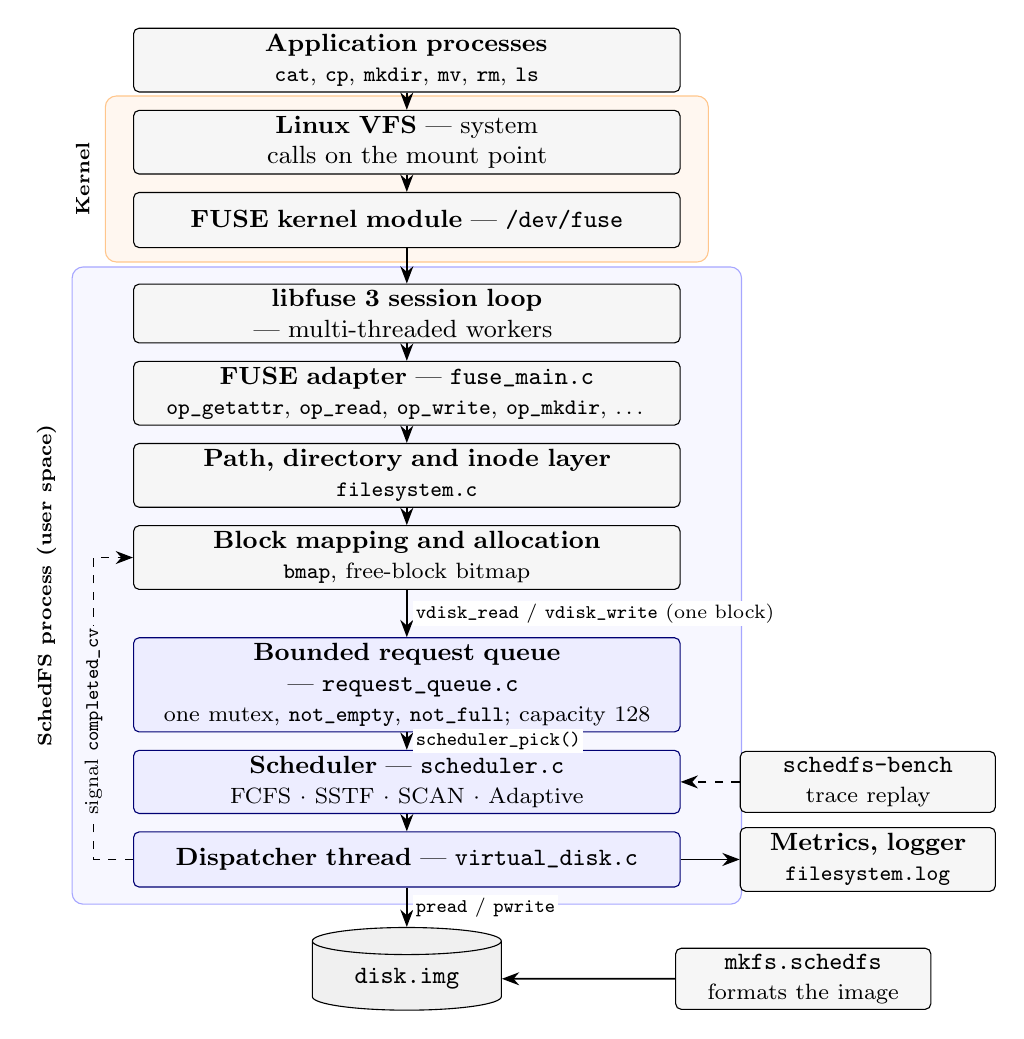
\begin{tikzpicture}[node distance=0.22cm, box/.append style={minimum height=0.7cm, inner sep=2pt}]
  \node[box=6.8cm] (app) {\textbf{Application processes}\\\footnotesize \code{cat}, \code{cp}, \code{mkdir}, \code{mv}, \code{rm}, \code{ls}};
  \node[box=6.8cm, below=of app] (vfs) {\textbf{Linux VFS} --- system calls on the mount point};
  \node[box=6.8cm, below=of vfs] (dev) {\textbf{FUSE kernel module} --- \code{/dev/fuse}};
  \node[box=6.8cm, below=0.45cm of dev] (lib) {\textbf{libfuse 3 session loop} --- multi-threaded workers};
  \node[box=6.8cm, below=of lib] (adp) {\textbf{FUSE adapter} --- \code{fuse_main.c}\\\footnotesize \code{op_getattr}, \code{op_read}, \code{op_write}, \code{op_mkdir}, \ldots};
  \node[box=6.8cm, below=of adp] (fsl) {\textbf{Path, directory and inode layer}\\\footnotesize \code{filesystem.c}};
  \node[box=6.8cm, below=of fsl] (map) {\textbf{Block mapping and allocation}\\\footnotesize \code{bmap}, free-block bitmap};
  \node[hbox=6.8cm, below=0.6cm of map] (q) {\textbf{Bounded request queue} --- \code{request_queue.c}\\\footnotesize one mutex, \code{not_empty}, \code{not_full}; capacity 128};
  \node[hbox=6.8cm, below=of q] (sch) {\textbf{Scheduler} --- \code{scheduler.c}\\\footnotesize FCFS $\cdot$ SSTF $\cdot$ SCAN $\cdot$ Adaptive};
  \node[hbox=6.8cm, below=of sch] (dsp) {\textbf{Dispatcher thread} --- \code{virtual_disk.c}};
  \node[store, below=0.5cm of dsp] (img) {\code{disk.img}};
  \node[box=3.1cm, right=0.75cm of dsp] (met) {\textbf{Metrics, logger}\\\footnotesize \code{filesystem.log}};
  \node[box=3.1cm, right=0.75cm of sch] (bench) {\textbf{\code{schedfs-bench}}\\\footnotesize trace replay};
  \node[box=3.1cm, right=2.2cm of img] (mk) {\textbf{\code{mkfs.schedfs}}\\\footnotesize formats the image};
  \foreach \a/\b in {app/vfs,vfs/dev,dev/lib,lib/adp,adp/fsl,fsl/map,sch/dsp}
    \draw[arr] (\a) -- (\b);
  \draw[arr] (map) -- node[lab, right=2pt] {\code{vdisk_read} / \code{vdisk_write} (one block)} (q);
  \draw[arr] (q) -- node[lab, right=2pt] {\code{scheduler_pick()}} (sch);
  \draw[arr] (dsp) -- node[lab, right=2pt] {\code{pread} / \code{pwrite}} (img);
  \draw[arr] (dsp) -- (met);
  \draw[arr, dashed] (bench) -- (sch);
  \draw[arr] (mk) -- (img);
  \draw[arr, dashed] (dsp.west) -- ++(-0.5,0) |- (map.west);
  \node[lab, rotate=90, fill=blue!3] at ($(dsp.west)+(-0.5,1.75)$) {signal \code{completed_cv}};
  \begin{scope}[on background layer]
    \node[fit=(vfs)(dev), inner xsep=10pt, inner ysep=5pt, fill=orange!6, draw=orange!45, rounded corners] (kern) {};
    \node[fit=(lib)(dsp), inner xsep=22pt, inner ysep=6pt, fill=blue!3, draw=blue!35, rounded corners] (user) {};
  \end{scope}
  \node[font=\scriptsize\bfseries, rotate=90, anchor=south] at ([xshift=-2pt]kern.west) {Kernel};
  \node[font=\scriptsize\bfseries, rotate=90, anchor=south] at ([xshift=-2pt]user.west) {SchedFS process (user space)};
\end{tikzpicture}
\caption{System architecture of SchedFS. Shaded blue layers are where scheduling takes place.}
\label{fig:arch}
\end{figure}

\figref{fig:deps} shows the component architecture as a dependency graph of the source modules. Arrows point from a module to the module whose interface it calls. The graph has no cycles: the scheduler depends only on the request definition, which is why the benchmark and the unit test can reuse it without a file system.

\begin{figure}[H]
\centering
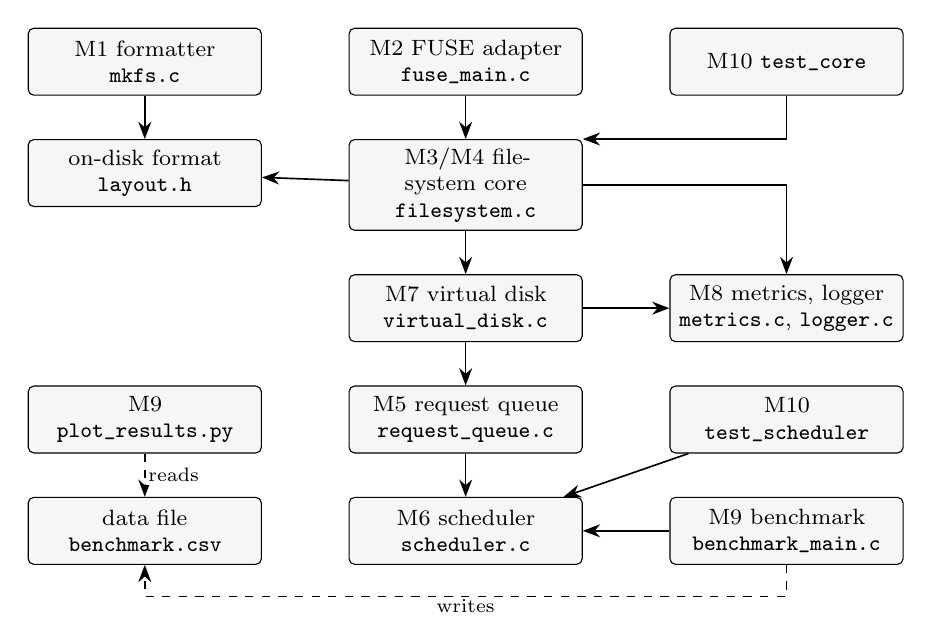
\begin{tikzpicture}[node distance=0.55cm and 0.7cm, m/.style={box=2.75cm, font=\footnotesize}]
  \node[m] (fuse) {M2 FUSE adapter\\\code{fuse_main.c}};
  \node[m, below=of fuse] (fs) {M3/M4 file-system core\\\code{filesystem.c}};
  \node[m, below=of fs] (vd) {M7 virtual disk\\\code{virtual_disk.c}};
  \node[m, below=of vd] (rq) {M5 request queue\\\code{request_queue.c}};
  \node[m, below=of rq] (sc) {M6 scheduler\\\code{scheduler.c}};
  \node[m, left=1.1cm of fuse] (mk) {M1 formatter\\\code{mkfs.c}};
  \node[m, below=of mk] (lay) {on-disk format\\\code{layout.h}};
  \node[m, right=1.1cm of vd] (met) {M8 metrics, logger\\\code{metrics.c}, \code{logger.c}};
  \node[m, right=1.1cm of sc] (bn) {M9 benchmark\\\code{benchmark_main.c}};
  \node[m, right=1.1cm of fuse] (tc) {M10 \code{test_core}};
  \node[m, right=1.1cm of rq] (ts) {M10 \code{test_scheduler}};
  \node[m, left=1.1cm of sc] (csv) {data file\\\code{benchmark.csv}};
  \node[m, above=0.55cm of csv] (py) {M9 \code{plot_results.py}};
  \draw[arr] (fuse) -- (fs); \draw[arr] (fs) -- (vd); \draw[arr] (vd) -- (rq); \draw[arr] (rq) -- (sc);
  \draw[arr] (mk) -- (lay); \draw[arr] (fs) -- (lay);
  \draw[arr] (vd) -- (met); \draw[arr] (fs.east) -| (met.north);
  \draw[arr] (bn) -- (sc); \draw[arr] (ts) -- (sc);
  \draw[arr] (tc) |- (fs.north east);
  \draw[arr, dashed] (bn.south) -- ++(0,-0.4) -| node[lab, pos=0.25, below] {writes} (csv.south);
  \draw[arr, dashed] (py) -- node[lab, right] {reads} (csv);
\end{tikzpicture}
\caption{Component architecture: dependencies between source modules (dashed: data files).}
\label{fig:deps}
\end{figure}

% ---------------------------------------------------------------------
\subsection{System Workflow}
\label{sec:workflow}
The life of a SchedFS instance has four phases: build, format, mount and serve, and unmount (\figref{fig:workflow}). Validation happens before FUSE takes over, so that every configuration error is printed in the terminal rather than lost inside a background process.

\begin{figure}[H]
\centering
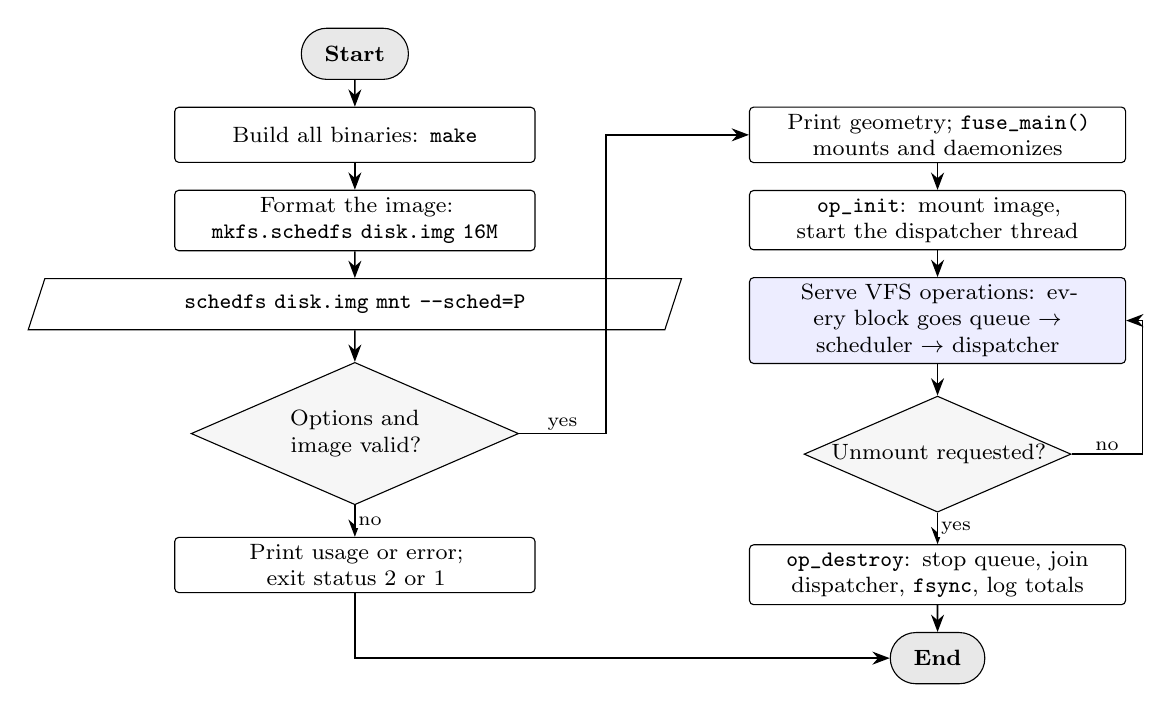
\begin{tikzpicture}[node distance=0.34cm]
  % left column: build, format, launch, validate
  \node[term] (s) {Start};
  \node[proc=4.4cm, below=of s] (b) {Build all binaries: \code{make}};
  \node[proc=4.4cm, below=of b] (f) {Format the image:\\\code{mkfs.schedfs disk.img 16M}};
  \node[io=4.4cm, below=of f] (m) {\code{schedfs disk.img mnt --sched=P}};
  \node[dec=2.7cm, below=0.4cm of m] (d1) {Options and image valid?};
  \node[proc=4.4cm, below=0.4cm of d1] (e) {Print usage or error;\\exit status 2 or 1};
  % right column: mount, serve, unmount
  \node[proc=4.6cm] (p) at ($(b)+(7.4,0)$) {Print geometry; \code{fuse_main()} mounts and daemonizes};
  \node[proc=4.6cm, below=of p] (i) {\code{op_init}: mount image, start the dispatcher thread};
  \node[proc=4.6cm, below=of i, fill=blue!7] (sv) {Serve VFS operations: every block goes queue $\rightarrow$ scheduler $\rightarrow$ dispatcher};
  \node[dec=2.7cm, below=0.4cm of sv] (d2) {Unmount requested?};
  \node[proc=4.6cm, below=0.4cm of d2] (de) {\code{op_destroy}: stop queue, join dispatcher, \code{fsync}, log totals};
  \node[term, below=of de] (t) {End};
  \foreach \a/\b in {s/b,b/f,f/m,m/d1,p/i,i/sv,sv/d2,de/t} \draw[arr] (\a) -- (\b);
  \draw[arr] (d1) -- node[lab, right] {no} (e);
  \draw[arr] (d1.east) -- node[lab, above] {yes} ++(1.1,0) |- (p.west);
  \draw[arr] (d2) -- node[lab, right] {yes} (de);
  \draw[arr] (d2.east) -- node[lab, above] {no} ++(0.9,0) |- (sv.east);
  \draw[arr] (e.south) |- (t.west);
\end{tikzpicture}
\caption{Overall workflow from build to unmount.}
\label{fig:workflow}
\end{figure}

\figref{fig:daemon} shows a detail of the mount phase that shaped the design. Without \code{-f}, \code{fuse_main()} daemonizes with \code{fork()}, and only the calling thread survives a \code{fork()}. If the dispatcher thread were created before \code{fuse_main()}, the daemon would have a request queue but nobody to empty it, and the first \code{mkdir} would block forever. SchedFS therefore validates the image in the foreground, releases it, and starts the real instance---including the dispatcher---in the FUSE \code{init} callback, which runs inside the daemon. The image path is converted to an absolute path first, because the daemon changes its working directory to \code{/}.

\begin{figure}[H]
\centering
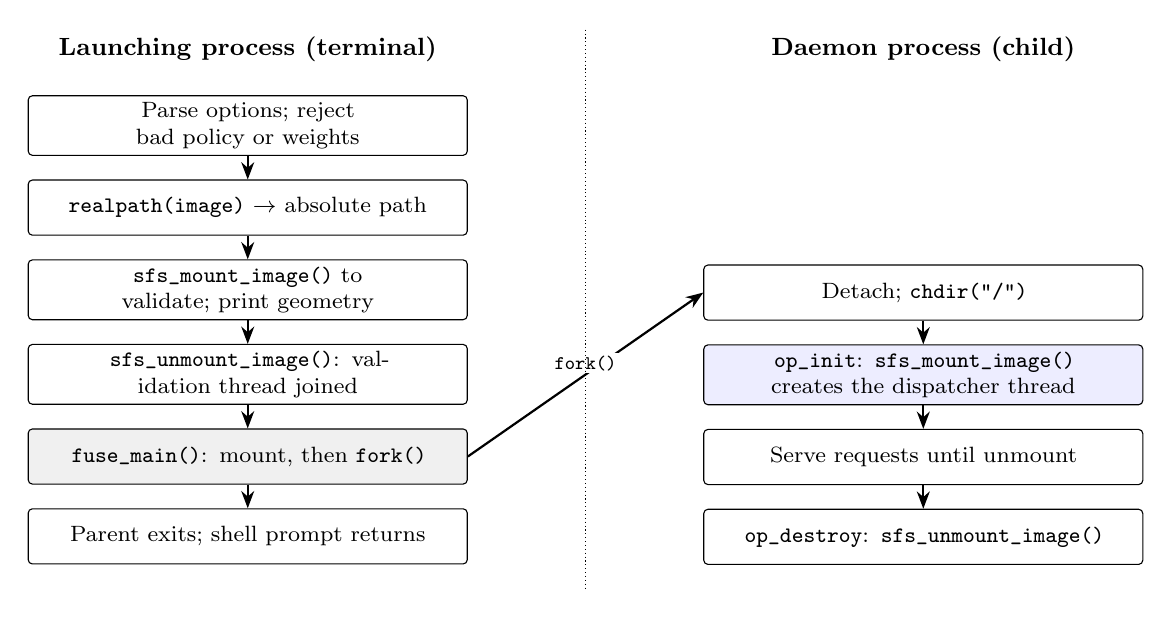
\begin{tikzpicture}[node distance=0.3cm]
  \node[font=\small\bfseries] (h1) {Launching process (terminal)};
  \node[proc=5.4cm, below=0.3cm of h1] (a1) {Parse options; reject bad policy or weights};
  \node[proc=5.4cm, below=of a1] (a2) {\code{realpath(image)} $\rightarrow$ absolute path};
  \node[proc=5.4cm, below=of a2] (a3) {\code{sfs_mount_image()} to validate; print geometry};
  \node[proc=5.4cm, below=of a3] (a4) {\code{sfs_unmount_image()}: validation thread joined};
  \node[proc=5.4cm, below=of a4, fill=gray!12] (a5) {\code{fuse_main()}: mount, then \code{fork()}};
  \node[proc=5.4cm, below=of a5] (a6) {Parent exits; shell prompt returns};
  \node[font=\small\bfseries, right=1.6cm of h1, xshift=2.4cm] (h2) {Daemon process (child)};
  \node[proc=5.4cm, below=2.45cm of h2] (b1) {Detach; \code{chdir("/")}};
  \node[proc=5.4cm, below=of b1, fill=blue!7] (b2) {\code{op_init}: \code{sfs_mount_image()} creates the dispatcher thread};
  \node[proc=5.4cm, below=of b2] (b3) {Serve requests until unmount};
  \node[proc=5.4cm, below=of b3] (b4) {\code{op_destroy}: \code{sfs_unmount_image()}};
  \foreach \a/\b in {a1/a2,a2/a3,a3/a4,a4/a5,a5/a6,b1/b2,b2/b3,b3/b4} \draw[arr] (\a) -- (\b);
  \draw[arr, thick] (a5.east) -- node[lab, above] {\code{fork()}} (b1.west);
  \draw[densely dotted] ($(h1)!0.5!(h2)+(0,0.25)$) -- ++(0,-7.1);
\end{tikzpicture}
\caption{Mount sequence. The dispatcher thread is created in \code{op_init}, after the fork.}
\label{fig:daemon}
\end{figure}

% ---------------------------------------------------------------------
\subsection{Module-Wise Design}
\label{sec:moddesign}

\subsubsection{On-disk format (M1, M3, M4)}
A 16~MiB image holds 4{,}096 blocks of 4{,}096 bytes (\figref{fig:layout}). Block~0 is the superblock, block~1 is the free-block bitmap (one bit per block, so one bitmap block covers 32{,}768 blocks), blocks 2--9 hold 256 inodes of 128 bytes each (32 per block), and blocks 10--4095 are data blocks. Block~10 is the root directory. \tabref{tab:superblock} decodes the first 64 bytes of a freshly formatted image, read with \code{od} in \figref{fig:term-mkfs}.

\begin{figure}[H]
\centering
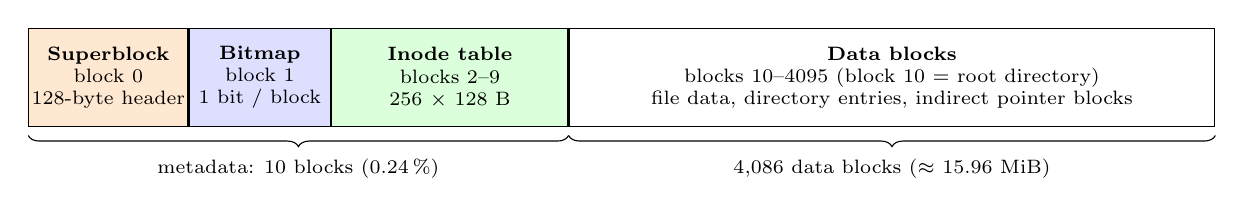
\begin{tikzpicture}[seg/.style={draw, minimum height=1.25cm, align=center, font=\scriptsize, inner sep=1pt}]
  \node[seg, fill=orange!18, minimum width=2.0cm, anchor=west] (sb) at (0,0) {\textbf{Superblock}\\block 0\\128-byte header};
  \node[seg, fill=blue!13, minimum width=1.8cm, anchor=west] (bm) at (sb.east) {\textbf{Bitmap}\\block 1\\1 bit / block};
  \node[seg, fill=green!14, minimum width=3.0cm, anchor=west] (it) at (bm.east) {\textbf{Inode table}\\blocks 2--9\\256 $\times$ 128 B};
  \node[seg, fill=white, minimum width=8.2cm, anchor=west] (db) at (it.east) {\textbf{Data blocks}\\blocks 10--4095 (block 10 = root directory)\\file data, directory entries, indirect pointer blocks};
  \draw[decorate, decoration={brace, amplitude=4pt, mirror}] ([yshift=-3pt]sb.south west) -- node[below=5pt, font=\scriptsize] {metadata: 10 blocks (0.24\,\%)} ([yshift=-3pt]it.south east);
  \draw[decorate, decoration={brace, amplitude=4pt, mirror}] ([yshift=-3pt]db.south west) -- node[below=5pt, font=\scriptsize] {4{,}086 data blocks ($\approx$ 15.96 MiB)} ([yshift=-3pt]db.south east);
\end{tikzpicture}
\caption{On-disk layout of a 16 MiB SchedFS image (widths not to scale).}
\label{fig:layout}
\end{figure}

\begin{table}[H]
\centering
\caption{Superblock of a freshly formatted 16 MiB image (values from \code{od}, \figref{fig:term-mkfs})}
\label{tab:superblock}
\small
\setlength{\tabcolsep}{4.5pt}
\begin{tabular}{@{}r l l l@{}}
\toprule
\textbf{Offset} & \textbf{Field} & \textbf{Value} & \textbf{Meaning} \\
\midrule
0 & \code{magic} & \code{0x53465331} & ASCII ``SFS1'' identifies a SchedFS image \\
4 & \code{version} & 1 & format version \\
8 & \code{block_size} & \code{0x1000} = 4096 & bytes per block \\
12 & \code{total_blocks} & \code{0x1000} = 4096 & 16 MiB / 4 KiB \\
16 & \code{free_blocks} & \code{0xff5} = 4085 & data blocks minus the root directory block \\
20 & \code{total_inodes} & \code{0x100} = 256 & fixed inode count \\
24 & \code{free_inodes} & \code{0xff} = 255 & all but the root inode \\
28, 32 & \code{bitmap_start}, \code{bitmap_blocks} & 1, 1 & bitmap location \\
36, 40 & \code{inode_start}, \code{inode_blocks} & 2, 8 & inode-table location \\
44 & \code{data_start} & \code{0xa} = 10 & first data block \\
48 & \code{root_inode} & 1 & inode number of \code{/} \\
\bottomrule
\end{tabular}
\end{table}

Each inode uses \emph{indexed allocation} with twelve direct pointers and one single-indirect pointer (\figref{fig:inode}), following the classic UNIX inode design \cite{bach1986}. The indirect block holds 1{,}024 four-byte block numbers, so a file can have $12 + 1024 = 1036$ blocks, or about 4.05~MiB. A pointer of zero marks a hole: reading it returns zeros without allocating a block, which is how a sparse \code{truncate} works.

\begin{figure}[H]
\centering
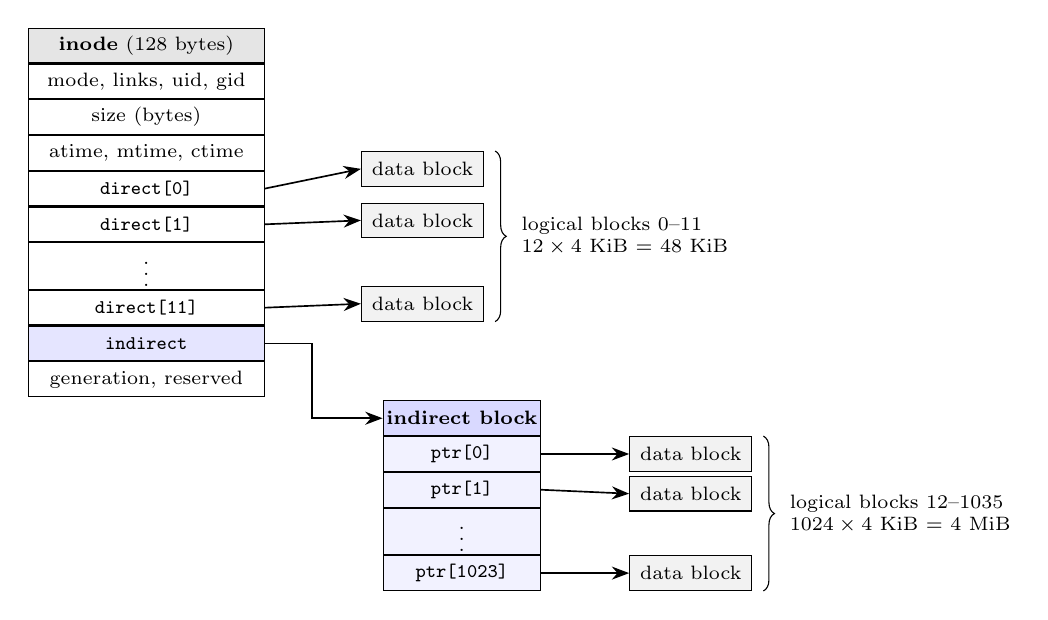
\begin{tikzpicture}[
    f/.style={draw, minimum width=3.0cm, minimum height=0.44cm, font=\scriptsize, fill=white, inner sep=1pt},
    db/.style={draw, fill=gray!10, minimum width=1.55cm, minimum height=0.44cm, font=\scriptsize, inner sep=1pt},
    pp/.style={draw, minimum width=2.0cm, minimum height=0.44cm, font=\scriptsize, fill=blue!5, inner sep=1pt}]
  \node[f, fill=gray!20] (h) at (0,0) {\textbf{inode} (128 bytes)};
  \node[f, below=0pt of h] (a) {mode, links, uid, gid};
  \node[f, below=0pt of a] (b) {size (bytes)};
  \node[f, below=0pt of b] (c) {atime, mtime, ctime};
  \node[f, below=0pt of c] (d0) {\code{direct[0]}};
  \node[f, below=0pt of d0] (d1) {\code{direct[1]}};
  \node[f, below=0pt of d1] (dd) {$\vdots$};
  \node[f, below=0pt of dd] (d11) {\code{direct[11]}};
  \node[f, below=0pt of d11, fill=blue!10] (ind) {\code{indirect}};
  \node[f, below=0pt of ind] (g) {generation, reserved};
  \node[db] (x0) at ($(d0.east)+(2.0,0.25)$) {data block};
  \node[db] (x1) at ($(d1.east)+(2.0,0.05)$) {data block};
  \node[db] (x11) at ($(d11.east)+(2.0,0.05)$) {data block};
  \draw[arr] (d0.east) -- (x0.west); \draw[arr] (d1.east) -- (x1.west); \draw[arr] (d11.east) -- (x11.west);
  \node[pp, fill=blue!15] (ph) at ($(ind.east)+(2.5,-0.95)$) {\textbf{indirect block}};
  \node[pp, below=0pt of ph] (p0) {\code{ptr[0]}};
  \node[pp, below=0pt of p0] (p1) {\code{ptr[1]}};
  \node[pp, below=0pt of p1] (pd) {$\vdots$};
  \node[pp, below=0pt of pd] (pn) {\code{ptr[1023]}};
  \draw[arr] (ind.east) -- ++(0.6,0) |- (ph.west);
  \node[db] (y0) at ($(p0.east)+(1.9,0)$) {data block};
  \node[db] (y1) at ($(p1.east)+(1.9,-0.05)$) {data block};
  \node[db] (yn) at ($(pn.east)+(1.9,0)$) {data block};
  \draw[arr] (p0.east) -- (y0.west); \draw[arr] (p1.east) -- (y1.west); \draw[arr] (pn.east) -- (yn.west);
  \draw[decorate, decoration={brace, amplitude=4pt}] ([xshift=4pt]x0.north east) -- node[right=6pt, font=\scriptsize, align=left] {logical blocks 0--11\\$12 \times 4$ KiB = 48 KiB} ([xshift=4pt]x11.south east);
  \draw[decorate, decoration={brace, amplitude=4pt}] ([xshift=4pt]y0.north east) -- node[right=6pt, font=\scriptsize, align=left] {logical blocks 12--1035\\$1024 \times 4$ KiB = 4 MiB} ([xshift=4pt]yn.south east);
\end{tikzpicture}
\caption{Inode structure and indexed allocation (12 direct pointers + 1 single-indirect block).}
\label{fig:inode}
\end{figure}

\subsubsection{Image formatter (M1)}
The formatter performs every check before it writes anything (\figref{fig:fc-mkfs}). Opening with \code{O_EXCL} makes it impossible to destroy an existing image by mistake, and any failure after creation removes the partly written file.

\begin{figure}[H]
\centering
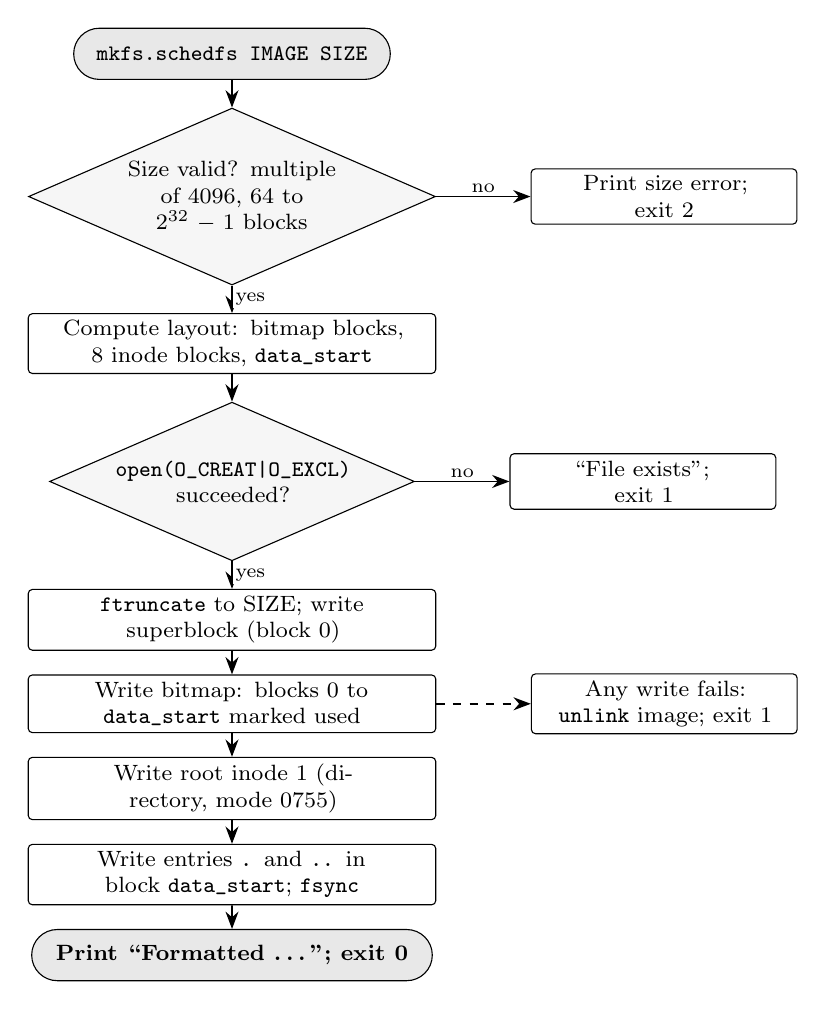
\begin{tikzpicture}[node distance=0.3cm]
  \node[term] (s) {\code{mkfs.schedfs IMAGE SIZE}};
  \node[dec=3.0cm, below=0.35cm of s] (d1) {Size valid? multiple of 4096, 64 to $2^{32}-1$ blocks};
  \node[proc=3.2cm, right=1.2cm of d1] (e1) {Print size error;\\exit 2};
  \node[proc=5.0cm, below=0.35cm of d1] (c) {Compute layout: bitmap blocks, 8 inode blocks, \code{data_start}};
  \node[dec=3.3cm, below=0.35cm of c] (d2) {\code{open(O_CREAT|O_EXCL)} succeeded?};
  \node[proc=3.2cm, right=1.2cm of d2] (e2) {``File exists'';\\exit 1};
  \node[proc=5.0cm, below=0.35cm of d2] (w1) {\code{ftruncate} to SIZE; write superblock (block 0)};
  \node[proc=5.0cm, below=of w1] (w2) {Write bitmap: blocks 0 to \code{data_start} marked used};
  \node[proc=5.0cm, below=of w2] (w3) {Write root inode 1 (directory, mode 0755)};
  \node[proc=5.0cm, below=of w3] (w4) {Write entries \code{.} and \code{..} in block \code{data_start}; \code{fsync}};
  \node[term, below=of w4] (t) {Print ``Formatted \ldots''; exit 0};
  \node[proc=3.2cm, right=1.2cm of w2] (e3) {Any write fails: \code{unlink} image; exit 1};
  \foreach \a/\b in {s/d1,c/d2,w1/w2,w2/w3,w3/w4,w4/t} \draw[arr] (\a) -- (\b);
  \draw[arr] (d1) -- node[lab, right] {yes} (c);
  \draw[arr] (d2) -- node[lab, right] {yes} (w1);
  \draw[arr] (d1) -- node[lab, above] {no} (e1);
  \draw[arr] (d2) -- node[lab, above] {no} (e2);
  \draw[arr, dashed] (w2) -- (e3);
\end{tikzpicture}
\caption{Flowchart of the image formatter (\code{mkfs/mkfs.c}).}
\label{fig:fc-mkfs}
\end{figure}

\subsubsection{Path resolution and the write path (M3, M4)}
Paths are resolved from the root, one component at a time (\figref{fig:fc-resolve}). A write (\figref{fig:fc-write}) holds the file's inode lock in exclusive mode, maps each logical block with \code{bmap(create = true)}, and reads the old block first only when the write covers part of it (read--modify--write). Size and modification time are written back once, at the end.

\begin{figure}[H]
\centering
\begin{minipage}[t]{0.42\linewidth}\centering
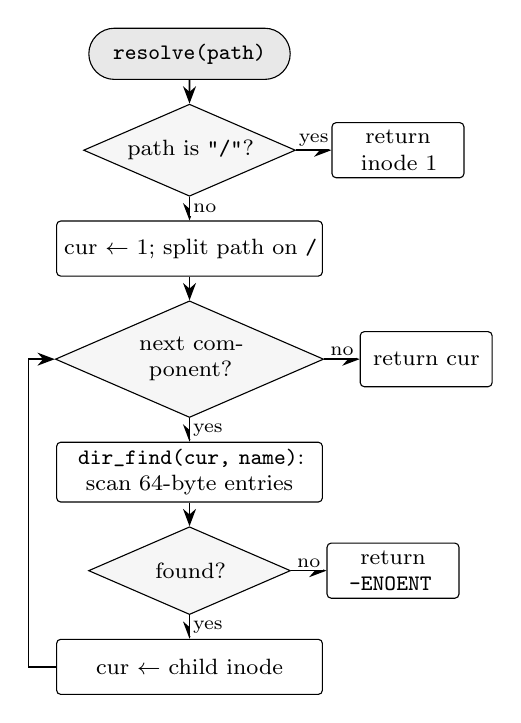
\begin{tikzpicture}[node distance=0.32cm]
  \node[term] (s) {\code{resolve(path)}};
  \node[dec=2.0cm, below=0.3cm of s] (d1) {path is \code{"/"}?};
  \node[proc=1.5cm, right=0.45cm of d1] (r1) {return inode 1};
  \node[proc=3.2cm, below=0.3cm of d1] (c) {cur $\leftarrow$ 1; split path on \code{/}};
  \node[dec=2.0cm, below=0.3cm of c] (d2) {next component?};
  \node[proc=1.5cm, right=0.45cm of d2] (r2) {return cur};
  \node[proc=3.2cm, below=0.3cm of d2] (f) {\code{dir_find(cur, name)}: scan 64-byte entries};
  \node[dec=2.0cm, below=0.3cm of f] (d3) {found?};
  \node[proc=1.5cm, right=0.45cm of d3] (r3) {return \code{-ENOENT}};
  \node[proc=3.2cm, below=0.3cm of d3] (n) {cur $\leftarrow$ child inode};
  \draw[arr] (s) -- (d1); \draw[arr] (d1) -- node[lab, above] {yes} (r1);
  \draw[arr] (d1) -- node[lab, right] {no} (c); \draw[arr] (c) -- (d2);
  \draw[arr] (d2) -- node[lab, above] {no} (r2); \draw[arr] (d2) -- node[lab, right] {yes} (f);
  \draw[arr] (f) -- (d3); \draw[arr] (d3) -- node[lab, above] {no} (r3);
  \draw[arr] (d3) -- node[lab, right] {yes} (n);
  \draw[arr] (n.west) -- ++(-0.35,0) |- (d2.west);
\end{tikzpicture}
\caption{Path resolution.}
\label{fig:fc-resolve}
\end{minipage}\hfill
\begin{minipage}[t]{0.55\linewidth}\centering
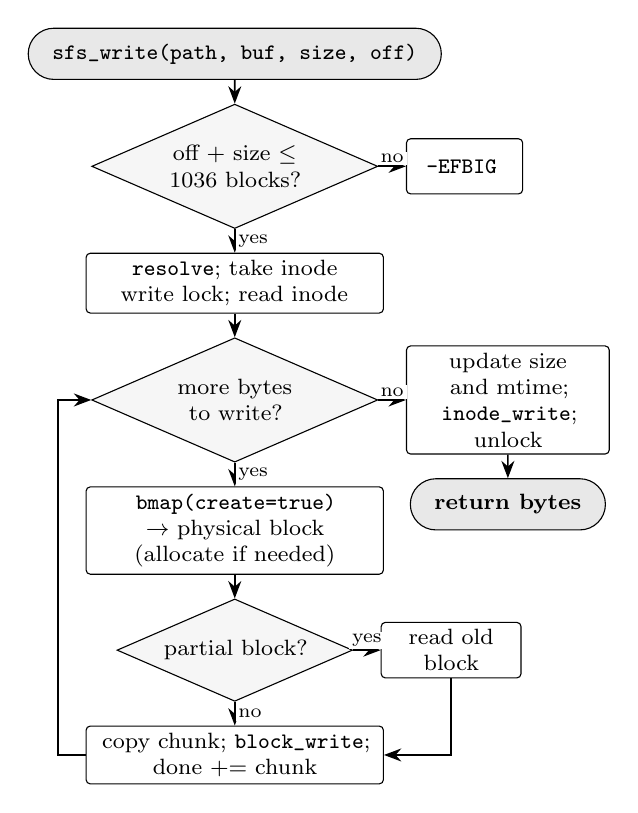
\begin{tikzpicture}[node distance=0.28cm]
  \node[term] (s) {\code{sfs_write(path, buf, size, off)}};
  \node[dec=2.3cm, below=0.3cm of s] (d0) {off + size $\le$ 1036 blocks?};
  \node[proc=1.3cm, right=0.35cm of d0] (e0) {\code{-EFBIG}};
  \node[proc=3.6cm, below=0.3cm of d0] (r) {\code{resolve}; take inode write lock; read inode};
  \node[dec=2.3cm, below=0.3cm of r] (d1) {more bytes to write?};
  \node[proc=3.6cm, below=0.3cm of d1] (bm) {\code{bmap(create=true)} $\rightarrow$ physical block (allocate if needed)};
  \node[dec=2.3cm, below=0.3cm of bm] (d2) {partial block?};
  \node[proc=1.6cm, right=0.35cm of d2] (rd) {read old block};
  \node[proc=3.6cm, below=0.3cm of d2] (wr) {copy chunk; \code{block_write}; done += chunk};
  \node[proc=2.4cm, right=0.35cm of d1] (fin) {update size and mtime; \code{inode_write}; unlock};
  \node[term, below=0.3cm of fin] (t) {return bytes};
  \draw[arr] (s) -- (d0); \draw[arr] (d0) -- node[lab, above] {no} (e0);
  \draw[arr] (d0) -- node[lab, right] {yes} (r); \draw[arr] (r) -- (d1);
  \draw[arr] (d1) -- node[lab, right] {yes} (bm); \draw[arr] (bm) -- (d2);
  \draw[arr] (d2) -- node[lab, above] {yes} (rd); \draw[arr] (rd) |- (wr.east);
  \draw[arr] (d2) -- node[lab, right] {no} (wr);
  \draw[arr] (wr.west) -- ++(-0.35,0) |- (d1.west);
  \draw[arr] (d1) -- node[lab, above] {no} (fin); \draw[arr] (fin) -- (t);
\end{tikzpicture}
\caption{Write path through M3 and M4.}
\label{fig:fc-write}
\end{minipage}
\end{figure}

\subsubsection{Block allocator (M4)}
\code{alloc_block()} looks for a free bit starting from a \emph{hint}: the physical block that holds the file's previous logical block (\figref{fig:fc-alloc}). Consecutive blocks of a file are therefore usually adjacent on disk. This keeps seek distances small for sequential access and makes the effect of scheduling easier to see. The Berkeley Fast File System applies the same locality principle \cite{mckusick1984}. The bitmap and superblock are written to disk before the block is used, and a failed write rolls the in-memory state back.

\begin{figure}[H]
\centering
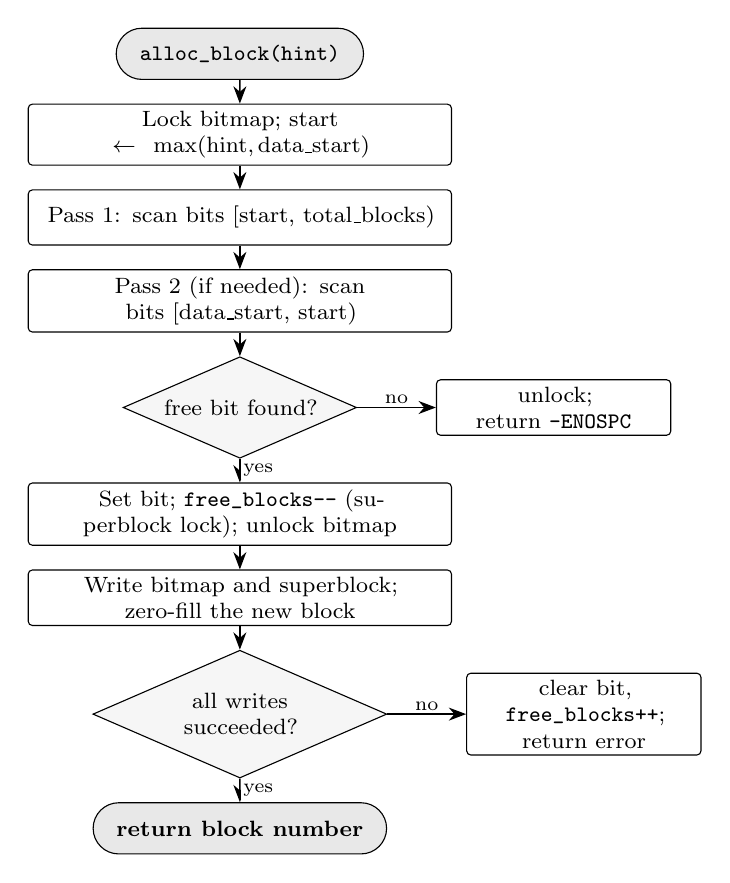
\begin{tikzpicture}[node distance=0.3cm]
  \node[term] (s) {\code{alloc_block(hint)}};
  \node[proc=5.2cm, below=0.3cm of s] (l) {Lock bitmap; start $\leftarrow \max(\text{hint}, \text{data\_start})$};
  \node[proc=5.2cm, below=of l] (p1) {Pass 1: scan bits [start, total\_blocks)};
  \node[proc=5.2cm, below=of p1] (p2) {Pass 2 (if needed): scan bits [data\_start, start)};
  \node[dec=2.4cm, below=0.3cm of p2] (d) {free bit found?};
  \node[proc=2.8cm, right=1.0cm of d] (e) {unlock;\\return \code{-ENOSPC}};
  \node[proc=5.2cm, below=0.3cm of d] (set) {Set bit; \code{free_blocks--} (superblock lock); unlock bitmap};
  \node[proc=5.2cm, below=of set] (w) {Write bitmap and superblock; zero-fill the new block};
  \node[dec=2.4cm, below=0.3cm of w] (d2) {all writes succeeded?};
  \node[proc=2.8cm, right=1.0cm of d2] (rb) {clear bit, \code{free_blocks++}; return error};
  \node[term, below=0.3cm of d2] (t) {return block number};
  \draw[arr] (s) -- (l); \draw[arr] (l) -- (p1); \draw[arr] (p1) -- (p2); \draw[arr] (p2) -- (d);
  \draw[arr] (d) -- node[lab, above] {no} (e); \draw[arr] (d) -- node[lab, right] {yes} (set);
  \draw[arr] (set) -- (w); \draw[arr] (w) -- (d2);
  \draw[arr] (d2) -- node[lab, above] {no} (rb); \draw[arr] (d2) -- node[lab, right] {yes} (t);
\end{tikzpicture}
\caption{Hint-based, two-pass block allocation.}
\label{fig:fc-alloc}
\end{figure}

\subsubsection{Bounded request queue (M5)}
The queue is the classic bounded buffer: producers wait while it is full, the consumer waits while it is empty, and every wait sits inside a \code{while} loop that re-checks its condition (\figref{fig:fc-queue}). A \code{stopping} flag lets unmount wake every waiter. Producers then receive \code{-ESHUTDOWN}, and the dispatcher receives \code{NULL} once the queue has drained.

\begin{figure}[H]
\centering
\begin{minipage}[t]{0.48\linewidth}\centering
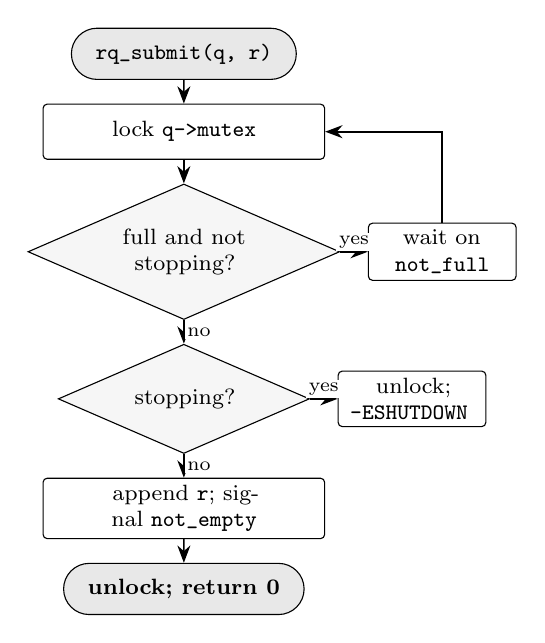
\begin{tikzpicture}[node distance=0.3cm]
  \node[term] (s) {\code{rq_submit(q, r)}};
  \node[proc=3.4cm, below=0.3cm of s] (l) {lock \code{q->mutex}};
  \node[dec=2.5cm, below=0.3cm of l] (d) {full and not stopping?};
  \node[proc=1.7cm, right=0.35cm of d] (w) {wait on \code{not_full}};
  \node[dec=2.5cm, below=0.3cm of d] (d2) {stopping?};
  \node[proc=1.7cm, right=0.35cm of d2] (e) {unlock; \code{-ESHUTDOWN}};
  \node[proc=3.4cm, below=0.3cm of d2] (a) {append \code{r}; signal \code{not_empty}};
  \node[term, below=of a] (t) {unlock; return 0};
  \draw[arr] (s) -- (l); \draw[arr] (l) -- (d);
  \draw[arr] (d) -- node[lab, above] {yes} (w); \draw[arr] (w.north) |- (l.east);
  \draw[arr] (d) -- node[lab, right] {no} (d2);
  \draw[arr] (d2) -- node[lab, above] {yes} (e);
  \draw[arr] (d2) -- node[lab, right] {no} (a); \draw[arr] (a) -- (t);
\end{tikzpicture}
\end{minipage}\hfill
\begin{minipage}[t]{0.48\linewidth}\centering
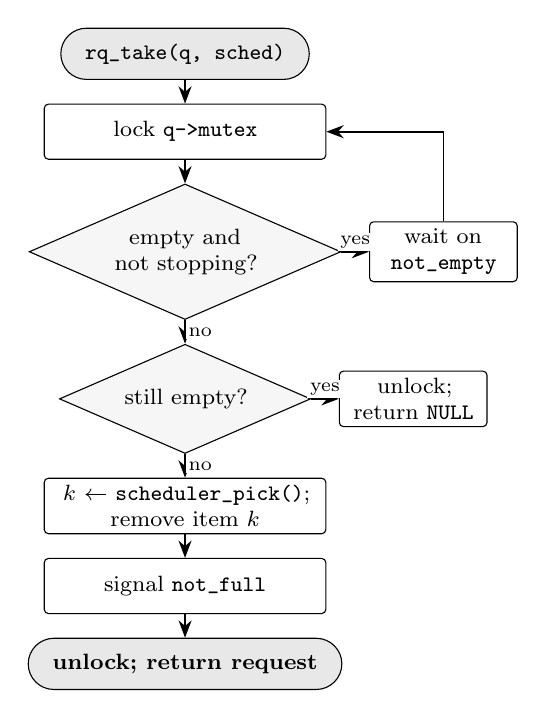
\begin{tikzpicture}[node distance=0.3cm]
  \node[term] (s) {\code{rq_take(q, sched)}};
  \node[proc=3.4cm, below=0.3cm of s] (l) {lock \code{q->mutex}};
  \node[dec=2.5cm, below=0.3cm of l] (d) {empty and not stopping?};
  \node[proc=1.7cm, right=0.35cm of d] (w) {wait on \code{not_empty}};
  \node[dec=2.5cm, below=0.3cm of d] (d2) {still empty?};
  \node[proc=1.7cm, right=0.35cm of d2] (e) {unlock; return \code{NULL}};
  \node[proc=3.4cm, below=0.3cm of d2] (a) {$k \leftarrow$ \code{scheduler_pick()}; remove item $k$};
  \node[proc=3.4cm, below=of a] (b) {signal \code{not_full}};
  \node[term, below=of b] (t) {unlock; return request};
  \draw[arr] (s) -- (l); \draw[arr] (l) -- (d);
  \draw[arr] (d) -- node[lab, above] {yes} (w); \draw[arr] (w.north) |- (l.east);
  \draw[arr] (d) -- node[lab, right] {no} (d2);
  \draw[arr] (d2) -- node[lab, above] {yes} (e);
  \draw[arr] (d2) -- node[lab, right] {no} (a); \draw[arr] (a) -- (b); \draw[arr] (b) -- (t);
\end{tikzpicture}
\end{minipage}
\caption{Producer side (left) and consumer side (right) of the bounded request queue.}
\label{fig:fc-queue}
\end{figure}

\subsubsection{Disk scheduler (M6)}
\code{scheduler_pick()} is a pure function: it reads the pending requests, the head position, the SCAN direction and the current time, and returns an index (\figref{fig:fc-sched}). It neither sleeps nor performs I/O, so it can run under the queue mutex and can be tested on its own. The four policies differ only in how they rank candidates; all of them break ties by arrival time and then request ID, which makes the service order deterministic.

\begin{figure}[H]
\centering
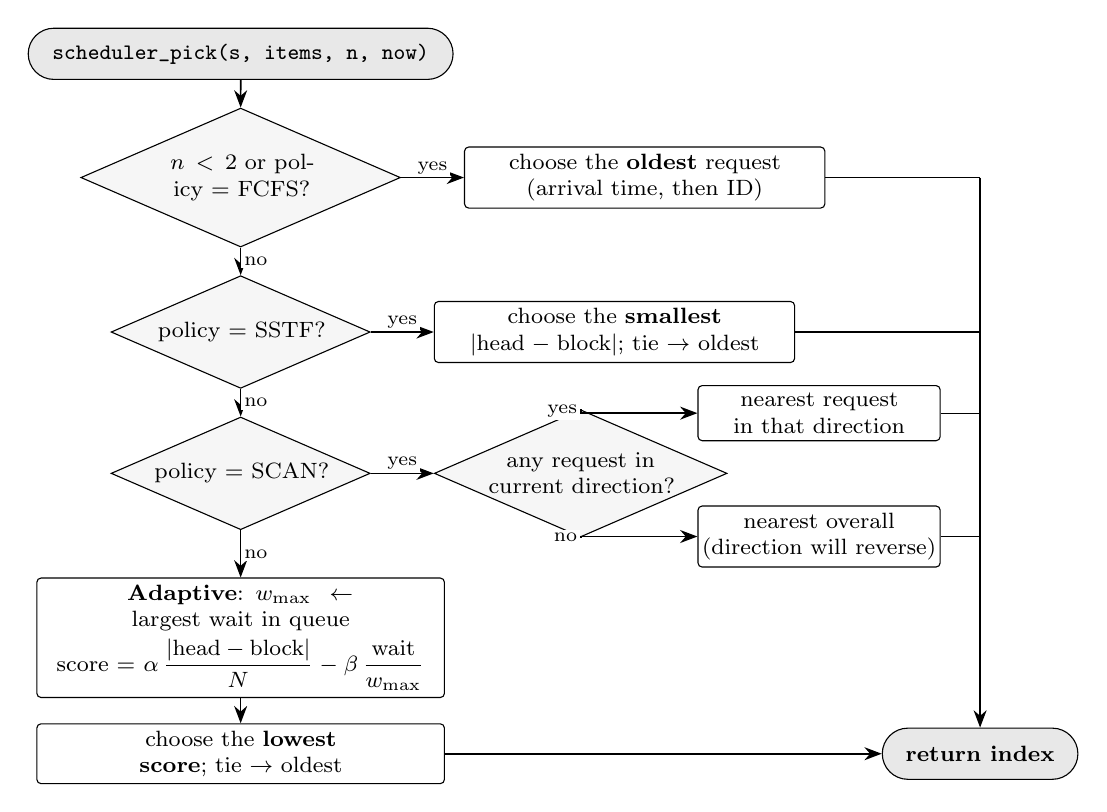
\begin{tikzpicture}[node distance=0.32cm]
  \node[term] (s) {\code{scheduler_pick(s, items, n, now)}};
  \node[dec=2.6cm, below=0.35cm of s] (d1) {$n < 2$ or policy = FCFS?};
  \node[proc=4.4cm, right=0.8cm of d1] (a1) {choose the \textbf{oldest} request (arrival time, then ID)};
  \node[dec=2.6cm, below=0.35cm of d1] (d2) {policy = SSTF?};
  \node[proc=4.4cm, right=0.8cm of d2] (a2) {choose the \textbf{smallest} $|\text{head} - \text{block}|$; tie $\rightarrow$ oldest};
  \node[dec=2.6cm, below=0.35cm of d2] (d3) {policy = SCAN?};
  \node[dec=2.4cm, right=0.8cm of d3] (d4) {any request in current direction?};
  \node[proc=2.9cm, above right=0.0cm and 0.55cm of d4] (a3) {nearest request in that direction};
  \node[proc=2.9cm, below right=0.0cm and 0.55cm of d4] (a4) {nearest overall (direction will reverse)};
  \node[proc=5.0cm, below=0.6cm of d3] (a5) {\textbf{Adaptive}: $w_{\max} \leftarrow$ largest wait in queue\\[2pt]
     score $= \alpha\, \dfrac{|\text{head}-\text{block}|}{N} - \beta\, \dfrac{\text{wait}}{w_{\max}}$};
  \node[proc=5.0cm, below=of a5] (a6) {choose the \textbf{lowest score}; tie $\rightarrow$ oldest};
  \coordinate (bus) at ($(a4.east)+(0.5,0)$);
  \node[term] (t) at (a6 -| bus) {return index};
  \draw[arr] (s) -- (d1);
  \draw[arr] (d1) -- node[lab, above] {yes} (a1);
  \draw[arr] (d1) -- node[lab, right] {no} (d2);
  \draw[arr] (d2) -- node[lab, above] {yes} (a2);
  \draw[arr] (d2) -- node[lab, right] {no} (d3);
  \draw[arr] (d3) -- node[lab, above] {yes} (d4);
  \draw[arr] (d4.north) |- node[lab, pos=0.3, left] {yes} (a3.west);
  \draw[arr] (d4.south) |- node[lab, pos=0.3, left] {no} (a4.west);
  \draw[arr] (d3) -- node[lab, right] {no} (a5);
  \draw[arr] (a5) -- (a6);
  \draw[arr] (a6) -- (t);
  \foreach \n in {a1,a2,a3,a4} \draw (\n.east) -- (\n.east -| bus);
  \draw[arr] (a1.east -| bus) -- (t.north);
\end{tikzpicture}
\caption{Decision logic of \code{scheduler_pick()} for the four policies.}
\label{fig:fc-sched}
\end{figure}

\subsubsection{Dispatcher (M7) and benchmark replay (M9)}
The dispatcher is the only consumer (\figref{fig:fc-dispatch}, left). After each transfer it records the seek distance and waiting time, moves the head to the served block, reverses the SCAN direction when the head has turned back, and wakes the waiting caller. The benchmark (\figref{fig:fc-dispatch}, right) reuses the same \code{scheduler_pick()} on fixed traces. All requests arrive at the start, so every policy sees identical input.

\begin{figure}[H]
\centering
\begin{minipage}[t]{0.48\linewidth}\centering
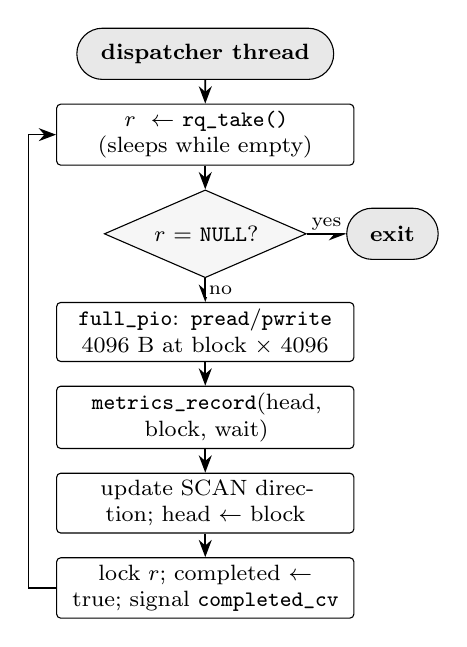
\begin{tikzpicture}[node distance=0.3cm]
  \node[term] (s) {dispatcher thread};
  \node[proc=3.6cm, below=0.3cm of s] (t) {$r \leftarrow$ \code{rq_take()} (sleeps while empty)};
  \node[dec=2.0cm, below=0.3cm of t] (d) {$r$ = \code{NULL}?};
  \node[term, right=0.5cm of d] (x) {exit};
  \node[proc=3.6cm, below=0.3cm of d] (io) {\code{full_pio}: \code{pread}/\code{pwrite} 4096 B at block $\times$ 4096};
  \node[proc=3.6cm, below=of io] (m) {\code{metrics_record}(head, block, wait)};
  \node[proc=3.6cm, below=of m] (h) {update SCAN direction; head $\leftarrow$ block};
  \node[proc=3.6cm, below=of h] (sg) {lock $r$; completed $\leftarrow$ true; signal \code{completed_cv}};
  \draw[arr] (s) -- (t); \draw[arr] (t) -- (d); \draw[arr] (d) -- node[lab, above] {yes} (x);
  \draw[arr] (d) -- node[lab, right] {no} (io); \draw[arr] (io) -- (m); \draw[arr] (m) -- (h); \draw[arr] (h) -- (sg);
  \draw[arr] (sg.west) -- ++(-0.35,0) |- (t.west);
\end{tikzpicture}
\end{minipage}\hfill
\begin{minipage}[t]{0.48\linewidth}\centering
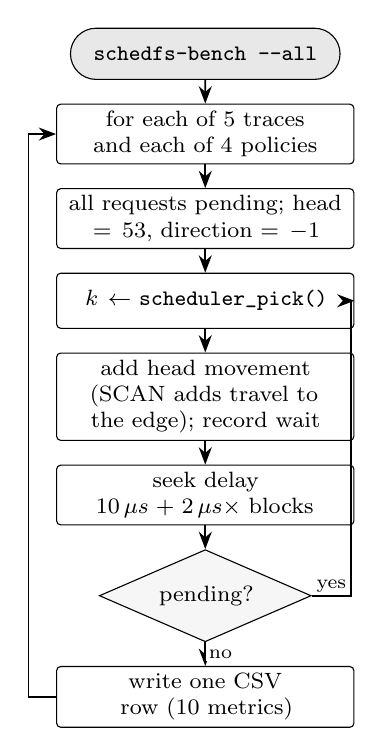
\begin{tikzpicture}[node distance=0.3cm]
  \node[term] (s) {\code{schedfs-bench --all}};
  \node[proc=3.6cm, below=0.3cm of s] (l) {for each of 5 traces and each of 4 policies};
  \node[proc=3.6cm, below=of l] (i) {all requests pending; head $= 53$, direction $= -1$};
  \node[proc=3.6cm, below=of i] (p) {$k \leftarrow$ \code{scheduler_pick()}};
  \node[proc=3.6cm, below=of p] (mv) {add head movement (SCAN adds travel to the edge); record wait};
  \node[proc=3.6cm, below=of mv] (sd) {seek delay $10\,\mu s + 2\,\mu s \times$ blocks};
  \node[dec=2.0cm, below=0.3cm of sd] (d) {pending?};
  \node[proc=3.6cm, below=0.3cm of d] (w) {write one CSV row (10 metrics)};
  \draw[arr] (s) -- (l); \draw[arr] (l) -- (i); \draw[arr] (i) -- (p); \draw[arr] (p) -- (mv); \draw[arr] (mv) -- (sd); \draw[arr] (sd) -- (d);
  \draw[arr] (d.east) -- node[lab, above] {yes} ++(0.5,0) |- (p.east);
  \draw[arr] (d) -- node[lab, right] {no} (w);
  \draw[arr] (w.west) -- ++(-0.35,0) |- (l.west);
\end{tikzpicture}
\end{minipage}
\caption{Dispatcher service loop (left) and benchmark replay loop (right).}
\label{fig:fc-dispatch}
\end{figure}

% ---------------------------------------------------------------------
\subsection{Module Interaction}
\label{sec:interaction}
\figref{fig:seq} follows one block read or write through the modules. The caller's request lives on the caller's own stack, and the dispatcher writes the data straight into the caller's buffer. No data is copied through the queue; only a pointer is passed. Because the caller sleeps on a condition variable that belongs to its own request, many threads can be waiting at once, and the scheduler always has a choice to make.

\begin{figure}[H]
\centering
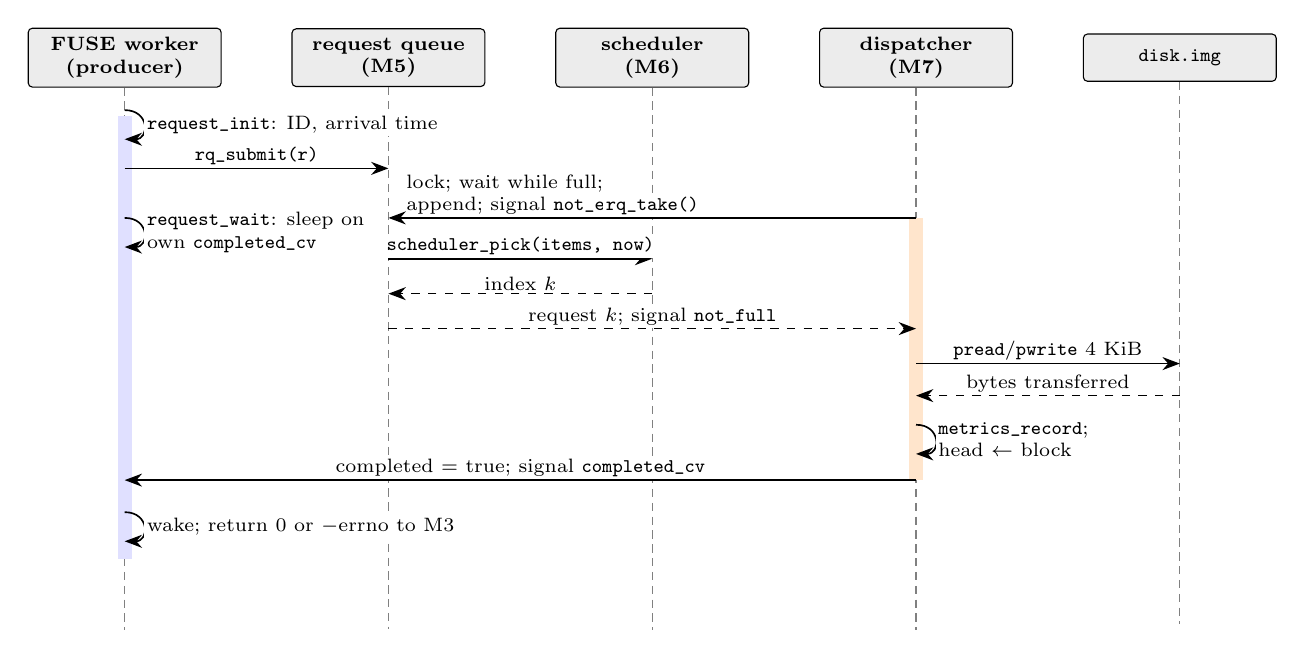
\begin{tikzpicture}[y=0.74cm,
    hd/.style={draw, fill=gray!15, rounded corners=1.5pt, font=\scriptsize\bfseries, minimum width=2.45cm, minimum height=0.6cm, align=center},
    msg/.style={->, semithick},
    m/.style={font=\scriptsize, fill=white, inner sep=1pt}]
  \foreach \x/\n/\t in {0/w/{FUSE worker\\(producer)}, 3.35/q/{request queue\\(M5)}, 6.7/sc/{scheduler\\(M6)}, 10.05/d/{dispatcher\\(M7)}, 13.4/img/{\code{disk.img}}} {
    \node[hd] (\n) at (\x,0) {\t};
    \draw[densely dashed, gray] (\n.south) -- ++(0,-9.3);
  }
  \fill[blue!12] (-0.09,-1.0) rectangle (0.09,-8.6);
  \fill[orange!20] (9.96,-2.75) rectangle (10.14,-7.25);
  \draw[msg] (0,-0.9) to[out=0,in=0,looseness=2.2] node[m, right] {\code{request_init}: ID, arrival time} (0,-1.4);
  \draw[msg] (0,-1.9) -- node[m, above] {\code{rq_submit(r)}} (3.35,-1.9);
  \node[m, align=left] at (5.1,-2.35) {lock; wait while full;\\append; signal \code{not_empty}};
  \draw[msg] (0,-2.75) to[out=0,in=0,looseness=2.2] node[m, right, align=left] {\code{request_wait}: sleep on\\own \code{completed_cv}} (0,-3.25);
  \draw[msg] (10.05,-2.75) -- node[m, above] {\code{rq_take()}} (3.35,-2.75);
  \draw[msg] (3.35,-3.45) -- node[m, above] {\code{scheduler_pick(items, now)}} (6.7,-3.45);
  \draw[msg, dashed] (6.7,-4.05) -- node[m, above] {index $k$} (3.35,-4.05);
  \draw[msg, dashed] (3.35,-4.65) -- node[m, above] {request $k$; signal \code{not_full}} (10.05,-4.65);
  \draw[msg] (10.05,-5.25) -- node[m, above] {\code{pread}/\code{pwrite} 4 KiB} (13.4,-5.25);
  \draw[msg, dashed] (13.4,-5.8) -- node[m, above] {bytes transferred} (10.05,-5.8);
  \draw[msg] (10.05,-6.3) to[out=0,in=0,looseness=2.2] node[m, right, align=left] {\code{metrics_record};\\head $\leftarrow$ block} (10.05,-6.8);
  \draw[msg] (10.05,-7.25) -- node[m, above] {completed $=$ true; signal \code{completed_cv}} (0,-7.25);
  \draw[msg] (0,-7.8) to[out=0,in=0,looseness=2.2] node[m, right] {wake; return 0 or $-$errno to M3} (0,-8.3);
\end{tikzpicture}
\caption{Sequence diagram of one scheduled block I/O.}
\label{fig:seq}
\end{figure}

\tabref{tab:interact} lists the interfaces through which the modules exchange information.

\begin{table}[H]
\centering
\caption{Interfaces between modules}
\label{tab:interact}
\small
\begin{tabularx}{\linewidth}{@{}l l X@{}}
\toprule
\textbf{From $\rightarrow$ To} & \textbf{Interface} & \textbf{Information exchanged} \\
\midrule
Kernel $\rightarrow$ M2 & \code{struct fuse_operations} & path, offset, size, buffer, mode, flags \\
M2 $\rightarrow$ M3 & \code{sfs_getattr}, \code{sfs_read}, \code{sfs_write}, \ldots & same arguments; returns bytes or \code{-errno} \\
M3 $\rightarrow$ M4 & \code{bmap}, \code{alloc_block}, \code{free_block} & inode, logical block, create flag $\rightarrow$ physical block \\
M3/M4 $\rightarrow$ M7 & \code{vdisk_read}, \code{vdisk_write} & block number, 4 KiB buffer pointer \\
M7 $\rightarrow$ M5 & \code{rq_submit}, \code{request_wait}, \code{rq_take} & pointer to \code{disk_request_t} \\
M5 $\rightarrow$ M6 & \code{scheduler_pick} & pending array, head, direction, time $\rightarrow$ index \\
M7 $\rightarrow$ M8 & \code{metrics_record}, \code{sfs_log} & from-block, to-block, wait (ms); log text \\
M9 $\rightarrow$ M6 & \code{scheduler_pick} & fixed traces $\rightarrow$ service order \\
M9 $\rightarrow$ files & \code{benchmark.csv} $\rightarrow$ \code{plot_results.py} & 10 metrics per (workload, policy) \\
\bottomrule
\end{tabularx}
\end{table}

% ---------------------------------------------------------------------
\subsection{Operating Systems Concepts}
\label{sec:osconcepts}

\subsubsection{Disk scheduling}
Each policy answers one question: \emph{which pending request should the head serve next?} \cite{teorey1972,silberschatz2018,stallings2018} \tabref{tab:policies} summarises the four answers. \figref{fig:headplot} plots the head position over time for the textbook trace (head at block 53, queue 98, 183, 37, 122, 14, 124, 65, 67 on a 200-block disk), using the exact service orders checked by \code{tests/test_scheduler.c}.

\begin{table}[H]
\centering
\caption{Scheduling policies implemented in \code{scheduler.c}}
\label{tab:policies}
\small
\begin{tabularx}{\linewidth}{@{}l X X X@{}}
\toprule
\textbf{Policy} & \textbf{Chooses next} & \textbf{Strength} & \textbf{Weakness} \\
\midrule
FCFS & the oldest request & fair; no starvation & ignores head position, so seeks are long \\
SSTF & the request nearest the head & short seeks & far requests can starve \\
SCAN & the nearest request in the current direction; reverses at the edge & sweeps evenly; bounded wait & extra travel to the edge \\
Adaptive & lowest $\alpha \cdot d/N - \beta \cdot w/w_{\max}$ & tunable between SSTF ($\beta = 0$) and age priority & sensitive to the scale of $d$ and $w$ \\
\bottomrule
\end{tabularx}
\end{table}

\begin{figure}[H]
\centering
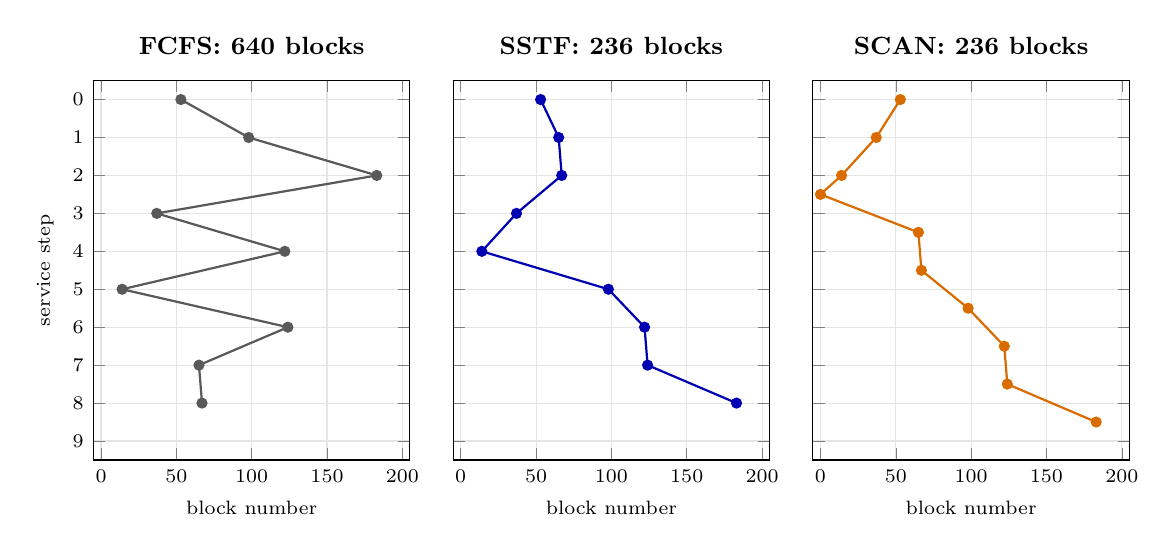
\begin{tikzpicture}
\begin{groupplot}[
    group style={group size=3 by 1, horizontal sep=0.55cm, yticklabels at=edge left},
    width=5.6cm, height=6.4cm, xmin=-5, xmax=205, ymin=-0.5, ymax=9.5, y dir=reverse,
    xtick={0,50,100,150,200}, ytick={0,...,9},
    xlabel={block number}, tick label style={font=\scriptsize}, label style={font=\scriptsize},
    title style={font=\small\bfseries}, grid=major, grid style={gray!20},
    every axis plot/.append style={thick, mark=*, mark size=1.6pt}]
  \nextgroupplot[title={FCFS: 640 blocks}, ylabel={service step}]
    \addplot[gray!70!black] coordinates {(53,0)(98,1)(183,2)(37,3)(122,4)(14,5)(124,6)(65,7)(67,8)};
  \nextgroupplot[title={SSTF: 236 blocks}]
    \addplot[blue!70!black] coordinates {(53,0)(65,1)(67,2)(37,3)(14,4)(98,5)(122,6)(124,7)(183,8)};
  \nextgroupplot[title={SCAN: 236 blocks}]
    \addplot[orange!85!black] coordinates {(53,0)(37,1)(14,2)(0,2.5)(65,3.5)(67,4.5)(98,5.5)(122,6.5)(124,7.5)(183,8.5)};
\end{groupplot}
\end{tikzpicture}
\caption{Head movement for the textbook trace. SCAN first moves towards block 0 and reaches the edge before reversing.}
\label{fig:headplot}
\end{figure}

\noindent The totals follow directly from the orders. For FCFS: $|98-53| + |183-98| + |37-183| + |122-37| + |14-122| + |124-14| + |65-124| + |67-65| = 45 + 85 + 146 + 85 + 108 + 110 + 59 + 2 = 640$. For SSTF: $12 + 2 + 30 + 23 + 84 + 24 + 2 + 59 = 236$. For SCAN, moving down first: $53 + 183 = 236$ (down to block~0, then up to block~183).

\subsubsection{The Adaptive policy and ageing}
SSTF minimises seek distance but can starve a request far from the head. FCFS never starves, but it ignores position. The Adaptive policy combines both quantities in one score:
\begin{equation}
\text{score}(r) \;=\; \alpha \,\frac{|\text{head} - \text{block}(r)|}{N} \;-\; \beta \,\frac{\text{now} - \text{arrival}(r)}{w_{\max}},
\label{eq:adaptive}
\end{equation}
where $N$ is the number of blocks on the disk, $w_{\max}$ is the longest current wait in the queue, and the request with the lowest score is served. Both terms are normalised to $[0,1]$. With $\beta = 0$ the policy is exactly SSTF. As $\beta$ grows, waiting time increasingly outweighs distance---a form of \emph{ageing}, the standard remedy for starvation \cite{silberschatz2018}. The defaults are $\alpha = 0.7$ and $\beta = 0.3$.

\subsubsection{Synchronization: bounded buffer, completion and reader--writer locks}
SchedFS uses three synchronization patterns from the course \cite{arpaci2018,posix2017,lewis1996,condwait}:
\begin{enumerate}[leftmargin=1.6em]
  \item \textbf{Bounded buffer (producer--consumer).} Many FUSE worker threads produce requests and one dispatcher consumes them. A mutex protects the array; condition variables \code{not_full} and \code{not_empty} block producers and the consumer respectively (\figref{fig:fc-queue}).
  \item \textbf{Completion signalling.} Each request carries its own mutex, condition variable and \code{completed} flag. The caller waits in \code{while (!completed) pthread_cond_wait(...)}, so a spurious wake-up is harmless and a signal cannot be lost: the flag is set under the same mutex before the signal is sent.
  \item \textbf{Reader--writer locks.} Each inode has a \code{pthread_rwlock_t}. Reads take it in shared mode, and writes and truncation take it in exclusive mode. Several readers of one file can therefore proceed in parallel, while a writer has exclusive access.
\end{enumerate}

\figref{fig:reqstate} shows the states a request passes through, including the blocking states created by these patterns.

\begin{figure}[H]
\centering
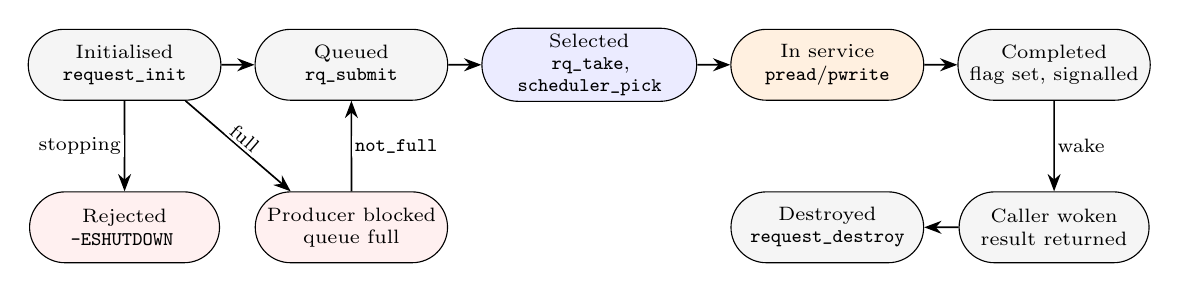
\begin{tikzpicture}[st/.style={draw, rounded rectangle, fill=gray!8, font=\scriptsize, align=center, minimum height=0.9cm, text width=2.15cm, inner sep=2pt}, node distance=0.42cm]
  \node[st] (i) {Initialised\\\code{request_init}};
  \node[st, right=of i] (q) {Queued\\\code{rq_submit}};
  \node[st, right=of q, fill=blue!8] (sel) {Selected\\\code{rq_take}, \code{scheduler_pick}};
  \node[st, right=of sel, fill=orange!12] (sv) {In service\\\code{pread}/\code{pwrite}};
  \node[st, right=of sv] (c) {Completed\\flag set, signalled};
  \node[st, below=1.15cm of c] (wk) {Caller woken\\result returned};
  \node[st, below=1.15cm of sv] (ds) {Destroyed\\\code{request_destroy}};
  \node[st, below=1.15cm of q, fill=red!6] (bf) {Producer blocked\\queue full};
  \node[st, below=1.15cm of i, fill=red!6] (sd) {Rejected\\\code{-ESHUTDOWN}};
  \draw[arr] (i) -- (q);
  \draw[arr] (q) -- (sel);
  \draw[arr] (sel) -- (sv);
  \draw[arr] (sv) -- (c);
  \draw[arr] (c) -- node[lab, right] {wake} (wk);
  \draw[arr] (wk) -- (ds);
  \draw[arr] (i.south east) -- node[lab, sloped, above] {full} (bf.north west);
  \draw[arr] (bf) -- node[lab, right] {\code{not_full}} (q);
  \draw[arr] (i) -- node[lab, left] {stopping} (sd);
\end{tikzpicture}
\caption{Life cycle of a disk request.}
\label{fig:reqstate}
\end{figure}

\subsubsection{Deadlock avoidance through lock ordering}
A thread that holds one lock and requests another can deadlock if another thread acquires the same two locks in the opposite order. SchedFS prevents this with one global order (\figref{fig:locks}), the standard prevention technique of breaking the circular-wait condition \cite{silberschatz2018}. Every code path that holds more than one lock acquires them in that order. A file-system thread may still hold its directory, inode or inode-table lock while it waits for a block request to complete. This cannot deadlock, because the dispatcher that completes the request takes only the queue mutex and the request's own completion mutex, neither of which is held by a waiting thread. The queue mutex is last in the order and is never held during \code{pread} or \code{pwrite}: the dispatcher removes the request and releases the mutex before the transfer.

\begin{figure}[H]
\centering
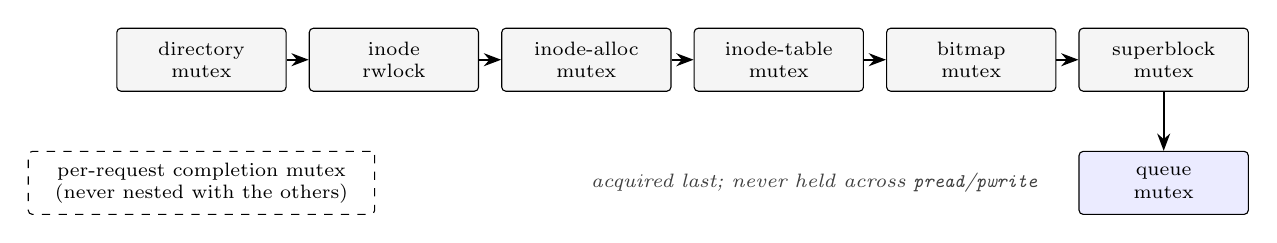
\begin{tikzpicture}[lk/.style={draw, fill=gray!8, rounded corners=1.5pt, font=\scriptsize, minimum width=2.15cm, minimum height=0.8cm, align=center, inner sep=1.5pt}, node distance=0.28cm]
  \node[lk] (l1) {directory\\mutex};
  \node[lk, right=of l1] (l2) {inode\\rwlock};
  \node[lk, right=of l2] (l3) {inode-alloc\\mutex};
  \node[lk, right=of l3] (l4) {inode-table\\mutex};
  \node[lk, right=of l4] (l5) {bitmap\\mutex};
  \node[lk, right=of l5] (l6) {superblock\\mutex};
  \node[lk, below=0.75cm of l6, fill=blue!8] (l7) {queue\\mutex};
  \foreach \a/\b in {l1/l2,l2/l3,l3/l4,l4/l5,l5/l6} \draw[arr] (\a) -- (\b);
  \draw[arr] (l6) -- (l7);
  \node[lk, below=0.75cm of l1, minimum width=4.4cm, fill=white, dashed] (rq) {per-request completion mutex\\(never nested with the others)};
  \node[note, left=0.4cm of l7, text width=6.8cm, align=right] {acquired last; never held across \code{pread}/\code{pwrite}};
\end{tikzpicture}
\caption{Global lock-acquisition order used to prevent deadlock.}
\label{fig:locks}
\end{figure}

\noindent The inode-table mutex was added after testing exposed a race. Thirty-two inodes share each 4~KiB table block, so updating one inode is a read--modify--write of the whole block. Without the mutex, two threads updating different inodes in the same block could each read the block, change their own inode and write it back, and one update would be lost. \code{test_core} detected this intermittently, and the mutex removed it.

\subsubsection{File systems and system calls}
SchedFS implements the textbook file-system abstractions on raw blocks \cite{arpaci2018,tanenbaum2015}: a superblock describing the layout, a free-space bitmap, fixed-size inodes with indexed allocation, directories as files of fixed-size entries, and path-name resolution. Through FUSE, the kernel turns each system call on the mount point (\code{open}, \code{read}, \code{write}, \code{mkdir}, \code{rename}, \code{stat}, \code{statfs}, \ldots) into a callback, and SchedFS answers with data or a negative \code{errno}. The project also illustrates process creation: daemonizing uses \code{fork()}, and only the calling thread survives it (\figref{fig:daemon}).

% ---------------------------------------------------------------------
\subsection{Data Flow}
\label{sec:dataflow}
\figref{fig:dfd} is a level-1 data-flow diagram. Circles are processes, open rectangles are data stores, and the plain rectangle is an external entity. Two separate flows exist. The \emph{live path} carries user data to and from the image. The \emph{evaluation path} carries fixed traces through the scheduler into \code{benchmark.csv} and then into graphs.

\begin{figure}[H]
\centering
\resizebox{\linewidth}{!}{%
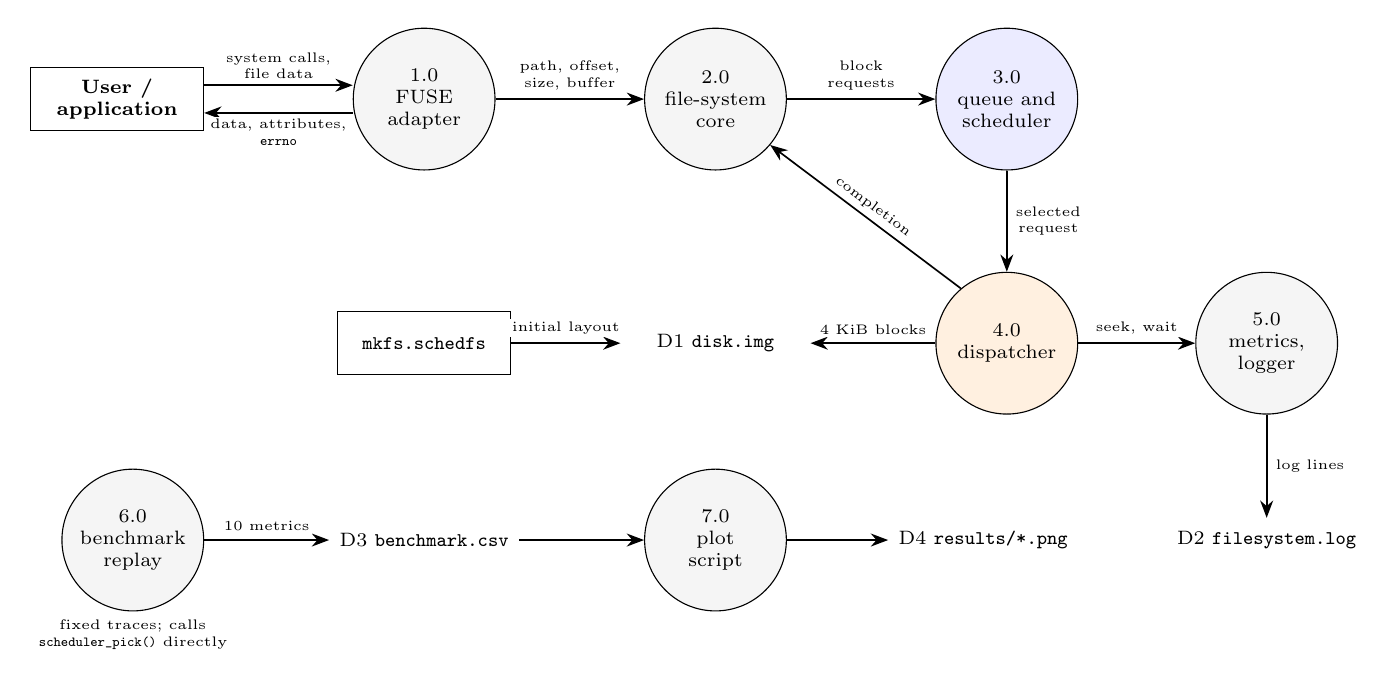
\begin{tikzpicture}[
    pr/.style={draw, circle, fill=gray!8, font=\scriptsize, align=center, minimum size=1.8cm, inner sep=1pt},
    ds/.style={draw=none, font=\scriptsize, minimum width=2.4cm, minimum height=0.55cm, append after command={
        [draw] (\tikzlastnode.north west) -- (\tikzlastnode.north east)
        (\tikzlastnode.south west) -- (\tikzlastnode.south east)}},
    ex/.style={draw, fill=white, font=\scriptsize\bfseries, minimum width=2.2cm, minimum height=0.8cm, align=center},
    fl/.style={->, semithick},
    fx/.style={font=\tiny, fill=white, inner sep=1pt, align=center}]
  % live path
  \node[ex] (user) at (0,0) {User /\\application};
  \node[pr] (p1) at (3.9,0) {1.0\\FUSE\\adapter};
  \node[pr] (p2) at (7.6,0) {2.0\\file-system\\core};
  \node[pr, fill=blue!8] (p3) at (11.3,0) {3.0\\queue and\\scheduler};
  \node[pr, fill=orange!12] (p4) at (11.3,-3.1) {4.0\\dispatcher};
  \node[ds] (img) at (7.6,-3.1) {D1 \code{disk.img}};
  \node[ex] (fmt) at (3.9,-3.1) {\code{mkfs.schedfs}};
  \node[pr] (p5) at (14.6,-3.1) {5.0\\metrics,\\logger};
  \node[ds] (log) at (14.6,-5.6) {D2 \code{filesystem.log}};
  % evaluation path
  \node[pr] (p6) at (0.2,-5.6) {6.0\\benchmark\\replay};
  \node[ds] (csv) at (3.9,-5.6) {D3 \code{benchmark.csv}};
  \node[pr] (p7) at (7.6,-5.6) {7.0\\plot\\script};
  \node[ds] (png) at (11.0,-5.6) {D4 \code{results/*.png}};
  \draw[fl] ([yshift=5pt]user.east) -- node[fx, above=1pt] {system calls,\\file data} ([yshift=5pt]p1.west);
  \draw[fl] ([yshift=-5pt]p1.west) -- node[fx, below=1pt] {data, attributes,\\\code{errno}} ([yshift=-5pt]user.east);
  \draw[fl] (p1) -- node[fx, above=2pt] {path, offset,\\size, buffer} (p2);
  \draw[fl] (p2) -- node[fx, above=2pt] {block\\requests} (p3);
  \draw[fl] (p3) -- node[fx, right=2pt] {selected\\request} (p4);
  \draw[fl] (p4) -- node[fx, above=2pt] {4 KiB blocks} (img);
  \draw[fl] (p4.130) -- node[fx, sloped, above=1pt] {completion} (p2.-40);
  \draw[fl] (fmt) -- node[fx, above=2pt] {initial layout} (img);
  \draw[fl] (p4) -- node[fx, above=2pt] {seek, wait} (p5);
  \draw[fl] (p5) -- node[fx, right=2pt] {log lines} (log);
  \draw[fl] (p6) -- node[fx, above=2pt] {10 metrics} (csv);
  \draw[fl] (csv) -- (p7);
  \draw[fl] (p7) -- (png);
  \node[fx, below=2pt of p6, text width=2.6cm] {fixed traces; calls \code{scheduler_pick()} directly};
\end{tikzpicture}}
\caption{Level-1 data-flow diagram.}
\label{fig:dfd}
\end{figure}

% ---------------------------------------------------------------------
\subsection{Design Decisions}
\label{sec:decisions}
\tabref{tab:decisions} records the main engineering choices, the alternatives considered and their consequences.

{\small
\begin{longtable}{@{}p{3.3cm}p{5.3cm}p{6.0cm}@{}}
\caption{Design decisions and trade-offs}\label{tab:decisions}\\
\toprule
\textbf{Decision} & \textbf{Reason} & \textbf{Trade-off or limitation} \\
\midrule
\endfirsthead
\toprule
\textbf{Decision} & \textbf{Reason} & \textbf{Trade-off or limitation} \\
\midrule
\endhead
\bottomrule
\endfoot
Single dispatcher thread & Makes ``head position'' meaningful and gives the scheduler full control of ordering. & No parallel I/O to the image; throughput is bounded by one thread. \\
Bounded queue (128 entries) & Back-pressure: producers block instead of consuming unlimited memory. & A burst larger than 128 requests makes producers wait. \\
Per-request condition variable & Each caller wakes only for its own request; no thundering herd. & One mutex and one condition variable per request. \\
Request on the caller's stack & No allocation per I/O; the buffer is written in place. & The caller must not return before completion, which \code{request_wait} guarantees. \\
Pure \code{scheduler_pick()} & Testable alone; reused by the benchmark and ported to the web demo. & The dispatcher, not the scheduler, must update head and direction. \\
Deterministic tie-breaking & Reproducible service orders and exact unit-test expectations. & Ties always favour older requests, a small bias. \\
Hint-based allocation & Keeps a file's blocks close together, so sequential access gives short seeks. & No defragmentation; free space can still fragment. \\
Write-through metadata & Bitmap and superblock are on disk before a block is used; simpler than a cache. & More I/O per allocation; no crash consistency without a journal. \\
Start dispatcher in \code{op_init} & Threads do not survive \code{fork()} during daemonization. & The image is opened twice (validation, then real mount). \\
Seek $= |\Delta\text{block}|$ & Matches the textbook model; independent of the host device. & Does not model rotation, SSD behaviour or device caches. \\
\end{longtable}
}
% =====================================================================
\section{IMPLEMENTATION DETAILS}
\label{sec:impl}
% =====================================================================

\subsection{Implementation Overview}
SchedFS is written in C11 and builds three executables from one source tree (\tabref{tab:tree}): the file system \code{schedfs}, the formatter \code{mkfs.schedfs} and the benchmark \code{schedfs-bench}. The headers in \code{include/} define every interface, so each \code{.c} file depends only on the layer directly below it. The execution flow follows \figref{fig:workflow}: \code{main()} in \code{fuse_main.c} validates the options and the image, \code{fuse_main()} hands control to libfuse, and from then on the program is driven by kernel callbacks on libfuse worker threads plus one dispatcher thread.

\begin{table}[H]
\centering
\caption{Source organisation}
\label{tab:tree}
\small
\begin{tabularx}{\linewidth}{@{}l l X@{}}
\toprule
\textbf{Directory} & \textbf{Files} & \textbf{Role} \\
\midrule
\code{include/} & 8 headers & on-disk format (\code{layout.h}) and the interface of every module \\
\code{src/fuse/} & \code{fuse_main.c} & option parsing, mount lifecycle, 16 FUSE callbacks \\
\code{src/fs/} & \code{filesystem.c} & inodes, directories, paths, bitmap allocation, block mapping \\
\code{src/sync/} & \code{request_queue.c} & request life cycle and the bounded queue \\
\code{src/sched/} & \code{scheduler.c} & FCFS, SSTF, SCAN and Adaptive selection \\
\code{src/storage/} & \code{virtual_disk.c} & image file, dispatcher thread, \code{pread}/\code{pwrite} \\
\code{src/bench/} & \code{benchmark_main.c}, \code{metrics.c} & trace replay, metric accumulation \\
\code{src/utils/} & \code{logger.c} & thread-safe levelled logging \\
\code{mkfs/} & \code{mkfs.c} & image formatter \\
\code{tests/} & 2 C tests, 1 shell script & scheduler, core and mounted system tests \\
\code{scripts/} & 2 Python scripts & graphs, workload generation \\
\code{docs/} & \code{index.html} and 3 Markdown files & interactive demo, architecture notes \\
\bottomrule
\end{tabularx}
\end{table}

\noindent The main data structures are listed in \tabref{tab:structs}. The three on-disk structures are packed, and their sizes are checked at compile time with \code{_Static_assert} (Listing~\ref{lst:layout}), so a change that alters the format fails to compile.

\begin{table}[H]
\centering
\caption{Principal data structures}
\label{tab:structs}
\small
\begin{tabularx}{\linewidth}{@{}l l X@{}}
\toprule
\textbf{Structure} & \textbf{Defined in} & \textbf{Key fields and purpose} \\
\midrule
\code{sfs_superblock_t} & \code{layout.h} & magic, geometry, free counts, region offsets; 128 bytes at block 0 \\
\code{sfs_inode_t} & \code{layout.h} & mode, links, owner, size, times, \code{direct[12]}, \code{indirect}; 128 bytes \\
\code{sfs_dirent_t} & \code{layout.h} & inode number and a 60-byte name; 64 entries per block \\
\code{disk_request_t} & \code{request.h} & ID, operation, block, buffer, arrival/service/completion times, mutex, condition variable, \code{completed}, result \\
\code{request_queue_t} & \code{request_queue.h} & array of request pointers, count, capacity, \code{stopping}, mutex, \code{not_empty}, \code{not_full} \\
\code{scheduler_t} & \code{scheduler.h} & policy, total blocks, head, SCAN direction, $\alpha$, $\beta$ \\
\code{virtual_disk_t} & \code{virtual_disk.h} & file descriptor, queue, scheduler, metrics, dispatcher thread \\
\code{sfs_t} & \code{filesystem.h} & disk, in-memory superblock and bitmap, global mutexes, 257 inode rwlocks, 257 directory mutexes \\
\bottomrule
\end{tabularx}
\end{table}

\subsection{Module-Wise Implementation}
\label{sec:modimpl}

\paragraph{M1 Image formatter.} \code{main()} in \code{mkfs/mkfs.c} validates the size with \code{parse_size()}, computes the layout (Listing~\ref{lst:mkfs}), and writes each region with \code{write_full()}, which repeats \code{pwrite} until every byte is written and retries on \code{EINTR}. Errors are reported with \code{perror}; any failure after the file is created jumps to a \code{fail:} label that closes and unlinks the image, so a half-formatted image is never left behind.

\paragraph{M2 FUSE adapter.} The callbacks are thin. Each one converts its arguments and returns the \code{sfs_*} result, which is already a negative \code{errno} as libfuse expects. The \code{init} and \code{destroy} callbacks (Listing~\ref{lst:fuseinit}) own the file-system instance. If the image cannot be mounted inside the daemon, \code{op_init} logs the error and calls \code{fuse_exit()}, so the process stops cleanly instead of serving a broken mount.

\paragraph{M3 Inode and directory layer.} Public operations follow one pattern: resolve the path, lock the inode in the right mode, read the inode, perform block operations, write the inode back and unlock. \code{inode_write} (Listing~\ref{lst:inodewrite}) is the read--modify--write that needed the inode-table mutex. \code{sfs_rename} (Listing~\ref{lst:rename}) shows the error-handling style for multi-step metadata changes: every step that succeeded is undone if a later step fails.

\paragraph{M4 Block allocation and mapping.} \code{bmap} (Listing~\ref{lst:bmap}) returns block 0 for an unallocated logical block when \code{create} is false, which is how holes read as zeros, and allocates on demand when \code{create} is true. \code{free_inode_blocks} releases direct blocks, then indirect entries, and finally the indirect block itself once it is empty.

\paragraph{M5 Request queue.} Listing~\ref{lst:queue} shows the two queue operations and the completion wait. Every \code{pthread_cond_wait} sits in a \code{while} loop that re-tests its predicate. Removal uses \code{memmove}, so the array keeps arrival order, which FCFS relies on.

\paragraph{M6 Scheduler.} Listing~\ref{lst:sched} is the complete selection function. \code{older()} gives the deterministic tie-break. SCAN falls back to the nearest request when nothing lies in the current direction; the dispatcher notices that the head has turned back and flips the direction.

\paragraph{M7 Virtual disk and dispatcher.} \code{transfer()} (Listing~\ref{lst:vdisk}) rejects out-of-range blocks with \code{EINVAL} before queuing anything. The dispatcher treats a short transfer as \code{EIO} and passes the error code back through the request, so a failure reaches the application as a normal \code{errno}.

\paragraph{M8 Metrics and logging.} \code{metrics_record} (Listing~\ref{lst:metrics}) accumulates the sum and sum of squares of the waiting times, so the mean and standard deviation can be computed without storing every sample. The logger serialises writes with a mutex and filters DEBUG entries unless \code{--verbose} is set.

\paragraph{M9 Benchmark.} The replay loop (Listing~\ref{lst:bench}) charges SCAN for travelling to the disk edge before it reverses (block 0 when moving down, block 4095 when moving up), which is what distinguishes SCAN's totals from LOOK's.

\paragraph{M10 Tests.} \code{test_scheduler} (Listing~\ref{lst:testsched}) asserts both the exact service order and the total head movement. \code{system.sh} adds a regression test for background mounting (Listing~\ref{lst:systemsh}); every step runs under \code{timeout}, so a hang fails the test instead of blocking it.

\subsection{Source Code}
\label{sec:source}
The listings below are copied verbatim from the repository, by line range, with the original line numbers. Complete files for the scheduling path are in Appendix~\ref{app:source}.

\lstinputlisting[firstline=21,lastline=45,caption={On-disk structures with compile-time size checks (\code{include/layout.h})},label={lst:layout}]{../include/layout.h}
\noindent The three \code{_Static_assert} lines tie the C structures to the on-disk format: 32 inodes and 64 directory entries fit exactly in one 4~KiB block.

\lstinputlisting[firstline=62,lastline=80,caption={Layout computation and safe creation of the image (\code{mkfs/mkfs.c})},label={lst:mkfs}]{../mkfs/mkfs.c}
\noindent For 4{,}096 blocks this gives one bitmap block, eight inode blocks and \code{data_start} $= 10$, which matches the output in \figref{fig:term-mkfs}.

\lstinputlisting[firstline=26,lastline=49,caption={Starting the file system inside the FUSE daemon (\code{src/fuse/fuse_main.c})},label={lst:fuseinit}]{../src/fuse/fuse_main.c}

\lstinputlisting[firstline=71,lastline=82,caption={Inode update protected by the inode-table mutex (\code{src/fs/filesystem.c})},label={lst:inodewrite}]{../src/fs/filesystem.c}

\lstinputlisting[firstline=185,lastline=226,caption={[Logical-to-physical block mapping (\code{filesystem.c})]Logical-to-physical block mapping with on-demand allocation (\code{src/fs/filesystem.c})},label={lst:bmap}]{../src/fs/filesystem.c}
\noindent Lines 191--192 pass the previous direct block as the allocation hint, which keeps a file's blocks adjacent (\figref{fig:fc-alloc}).

\lstinputlisting[firstline=733,lastline=767,caption={Rename with roll-back of completed steps on failure (\code{src/fs/filesystem.c})},label={lst:rename}]{../src/fs/filesystem.c}

\lstinputlisting[firstline=39,lastline=93,caption={[Completion wait and bounded queue (\code{request_queue.c})]Completion wait and the bounded producer--consumer queue (\code{src/sync/request_queue.c})},label={lst:queue}]{../src/sync/request_queue.c}
\noindent The scheduler runs at line 86 while the queue mutex is held, which is safe because \code{scheduler_pick} never blocks. The I/O itself happens after \code{rq_take} has released the mutex.

\lstinputlisting[firstline=37,lastline=106,caption={Request selection for all four policies (\code{src/sched/scheduler.c})},label={lst:sched}]{../src/sched/scheduler.c}
\noindent Lines 88--105 implement Equation~\eqref{eq:adaptive}. The $10^{-12}$ tolerance makes equal scores compare as equal despite floating-point rounding, so the tie-break still applies.

\lstinputlisting[firstline=32,lastline=96,caption={[Dispatcher thread and synchronous transfer (\code{virtual_disk.c})]Dispatcher thread and the synchronous transfer used by the file system (\code{src/storage/virtual_disk.c})},label={lst:vdisk}]{../src/storage/virtual_disk.c}

\lstinputlisting[firstline=16,lastline=26,caption={Thread-safe metric accumulation (\code{src/bench/metrics.c})},label={lst:metrics}]{../src/bench/metrics.c}

\lstinputlisting[firstline=74,lastline=96,caption={Replay loop and SCAN edge accounting (\code{src/bench/benchmark_main.c})},label={lst:bench}]{../src/bench/benchmark_main.c}

\lstinputlisting[firstline=11,lastline=48,caption={Textbook-trace unit test (\code{tests/test_scheduler.c})},label={lst:testsched}]{../tests/test_scheduler.c}

\lstinputlisting[style=shstyle,firstline=20,lastline=34,caption={Background-mount regression test (\code{tests/system.sh})},label={lst:systemsh}]{../tests/system.sh}

% ---------------------------------------------------------------------
\subsection{Code Contribution Summary}
\label{sec:loc}
\textbf{Counting method.} Lines were counted with \code{report/tools/count_loc.py}, which is included in the repository with this report. It reads every C source and header, shell script, Python script and the Makefile in the repository, and it skips blank lines and comment-only lines. C block comments are removed before counting. Generated files, third-party code, \code{docs/}, \code{results/}, this \code{report/} folder and the 655-line HTML demo page are excluded. The result is \textbf{2{,}103 qualifying lines} (2{,}369 physical lines), well above the required $4 \times 300 = 1{,}200$. \tabref{tab:locfile} gives the per-file counts.

{\small
\begin{longtable}{@{}l r r l@{}}
\caption{Qualifying lines of code per file}\label{tab:locfile}\\
\toprule
\textbf{File} & \textbf{Qualifying} & \textbf{Physical} & \textbf{Module} \\
\midrule
\endfirsthead
\toprule
\textbf{File} & \textbf{Qualifying} & \textbf{Physical} & \textbf{Module} \\
\midrule
\endhead
\bottomrule
\endfoot
\code{src/fs/filesystem.c} & 773 & 814 & M3, M4 \\
\code{src/fuse/fuse_main.c} & 199 & 234 & M2 \\
\code{mkfs/mkfs.c} & 145 & 154 & M1 \\
\code{src/bench/benchmark_main.c} & 130 & 142 & M9 \\
\code{src/storage/virtual_disk.c} & 103 & 116 & M7 \\
\code{src/sched/scheduler.c} & 95 & 106 & M6 \\
\code{src/sync/request_queue.c} & 94 & 108 & M5 \\
\code{tests/test_core.c} & 91 & 100 & M10 \\
\code{scripts/plot_results.py} & 88 & 108 & M9 \\
\code{tests/test_scheduler.c} & 42 & 49 & M10 \\
\code{src/utils/logger.c} & 40 & 49 & M8 \\
\code{Makefile} & 35 & 36 & M10 \\
\code{include/filesystem.h} & 35 & 43 & M3, M4 \\
\code{include/layout.h} & 35 & 47 & M1 \\
\code{include/request.h} & 35 & 44 & M5 \\
\code{tests/system.sh} & 32 & 34 & M10 \\
\code{scripts/generate_workload.py} & 28 & 38 & M9 \\
\code{src/bench/metrics.c} & 21 & 29 & M8 \\
\code{include/virtual_disk.h} & 21 & 28 & M7 \\
\code{include/request_queue.h} & 20 & 27 & M5 \\
\code{include/scheduler.h} & 18 & 26 & M6 \\
\code{include/metrics.h} & 15 & 22 & M8 \\
\code{include/logger.h} & 8 & 15 & M8 \\
\midrule
\textbf{Total} & \textbf{2{,}103} & \textbf{2{,}369} & \\
\end{longtable}
}

\noindent\textbf{Attribution.} The Git history of the repository records every commit under one account, so individual authorship cannot be established from the repository alone. \tabref{tab:contrib} therefore gives a \emph{proposed} allocation of modules to members. It is based on module boundaries and gives each member at least 300 verified lines, and it must be confirmed by the team before submission.

\begin{table}[H]
\centering
\caption{Code contribution summary (proposed allocation, for team verification)}
\label{tab:contrib}
\small
\begin{tabularx}{\linewidth}{@{}l X r r l@{}}
\toprule
\textbf{Member} & \textbf{Assigned modules and files} & \textbf{LOC} & \textbf{Min.} & \textbf{Status} \\
\midrule
Saanvi Grover & M1, M2, M8 logger: \code{fuse_main.c}, \code{mkfs.c}, \code{layout.h}, \code{filesystem.h}, \code{logger.c/.h}, \code{system.sh} & 494 & 300 & Meets$^{*}$ \\
Prankit Goel & M5, M6, M7: \code{request_queue.c}, \code{scheduler.c}, \code{virtual_disk.c}, their headers, \code{test_scheduler.c} & 428 & 300 & Meets$^{*}$ \\
Aditya Sharma & M3, M4: \code{filesystem.c} & 773 & 300 & Meets$^{*}$ \\
Aaradhya Shankar Kulashri & M8 metrics, M9, M10: \code{benchmark_main.c}, \code{metrics.c/.h}, both Python scripts, \code{test_core.c}, \code{Makefile} & 408 & 300 & Meets$^{*}$ \\
\midrule
\textbf{Team} & all modules & \textbf{2{,}103} & \textbf{1{,}200} & \textbf{Meets} \\
\bottomrule
\end{tabularx}
\par\smallskip\raggedright\footnotesize $^{*}$Line counts are verified by script; the assignment of files to members is a proposal to be confirmed by the team.
\end{table}

% ---------------------------------------------------------------------
\subsection{Implementation Screenshots}
\label{sec:implshots}
All terminal figures in this report come from one run of the repository at commit \code{a7e489c} in an \code{ubuntu:24.04} container with \code{/dev/fuse}, executed as the unprivileged user \code{student}. Each figure is drawn from the captured terminal text without editing; the raw logs are kept in \code{figures/screenshots/raw_logs/}. The browser figures are screenshots of the live demo page.

\begin{figure}[H]
\centering
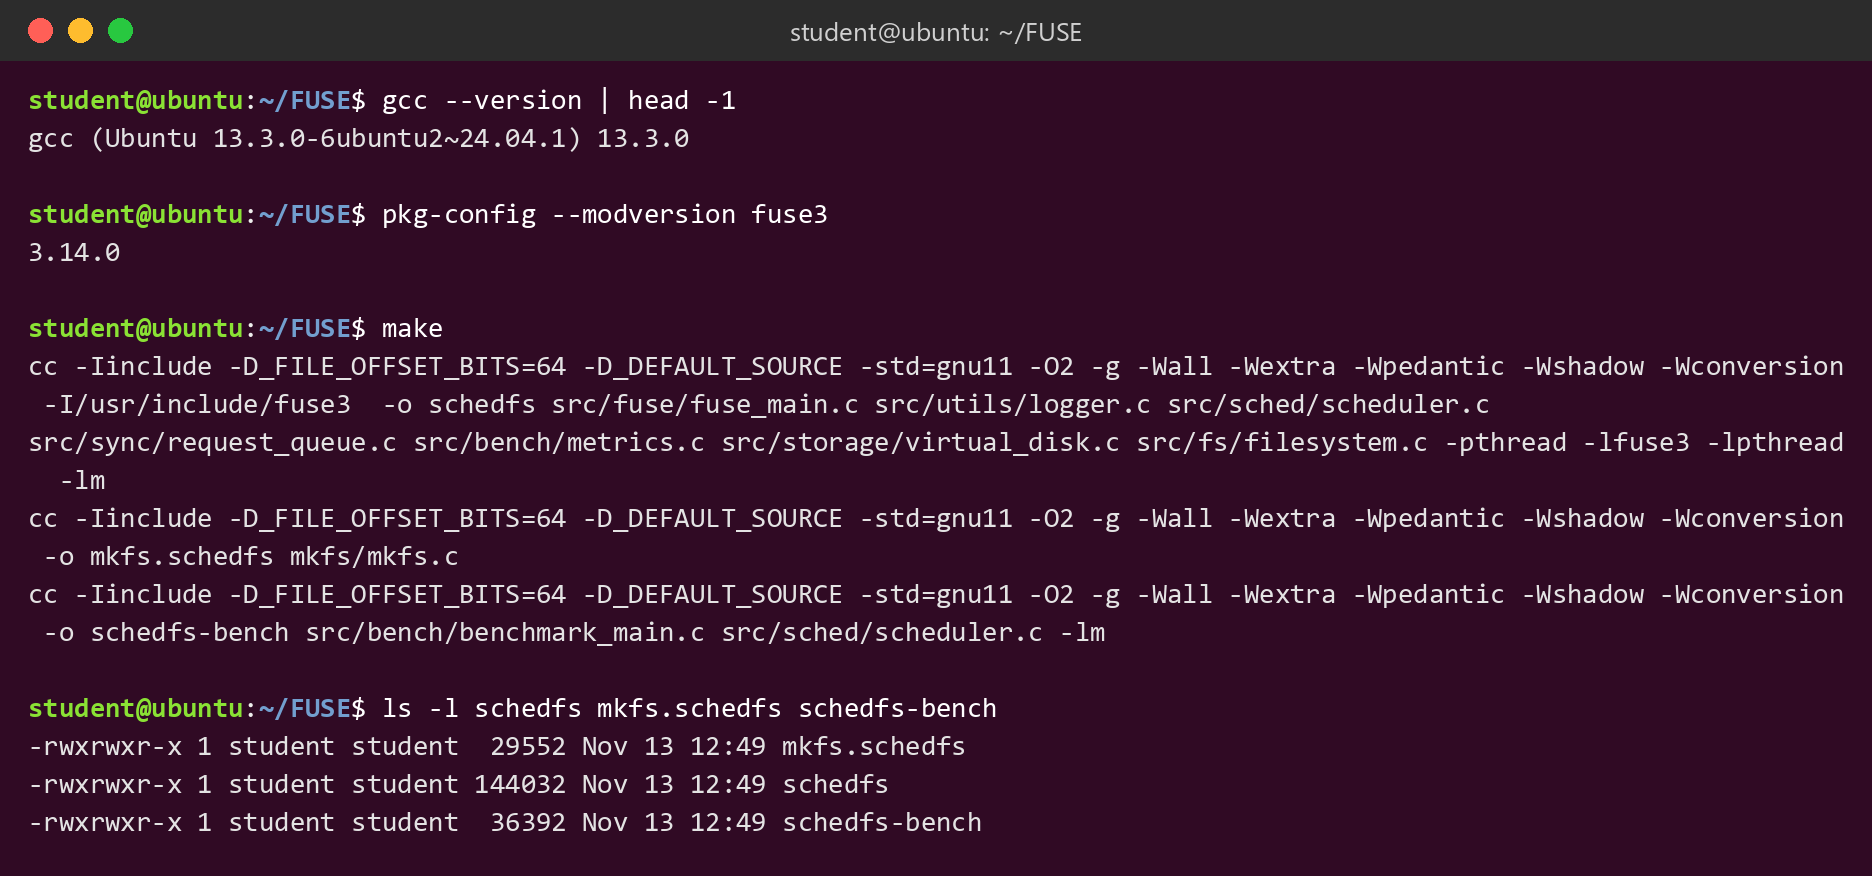
\includegraphics[width=\linewidth]{figures/screenshots/term_01_build.png}
\caption{Building the three executables with strict warning flags; the compiler emits no warnings.}
\label{fig:term-build}
\end{figure}

\begin{figure}[H]
\centering
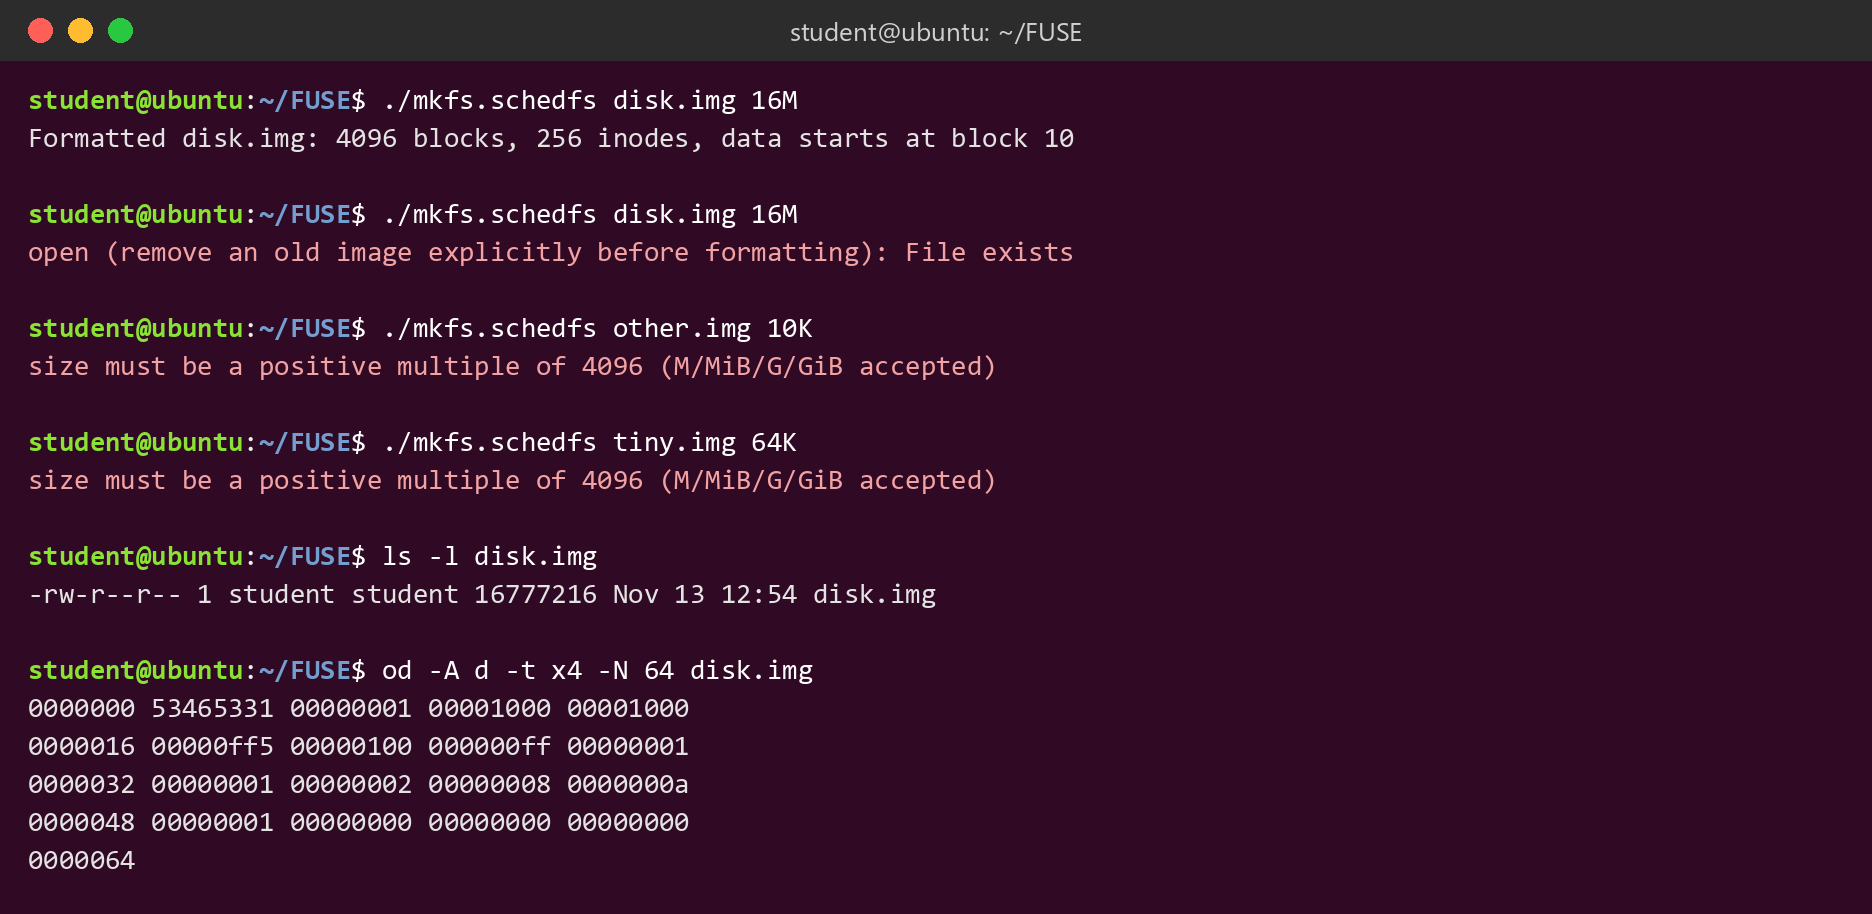
\includegraphics[width=\linewidth]{figures/screenshots/term_02_mkfs.png}
\caption{Formatting an image, refusing to overwrite it, rejecting invalid sizes, and dumping the superblock.}
\label{fig:term-mkfs}
\end{figure}

\noindent \figref{fig:term-mkfs} shows FR1 at work. The second \code{mkfs} is refused because the image exists. The sizes \code{10K} and \code{64K} are both rejected because the formatter accepts only the suffixes M, MiB, G and GiB; the message says so. The \code{od} dump is decoded in \tabref{tab:superblock}.

\begin{figure}[H]
\centering
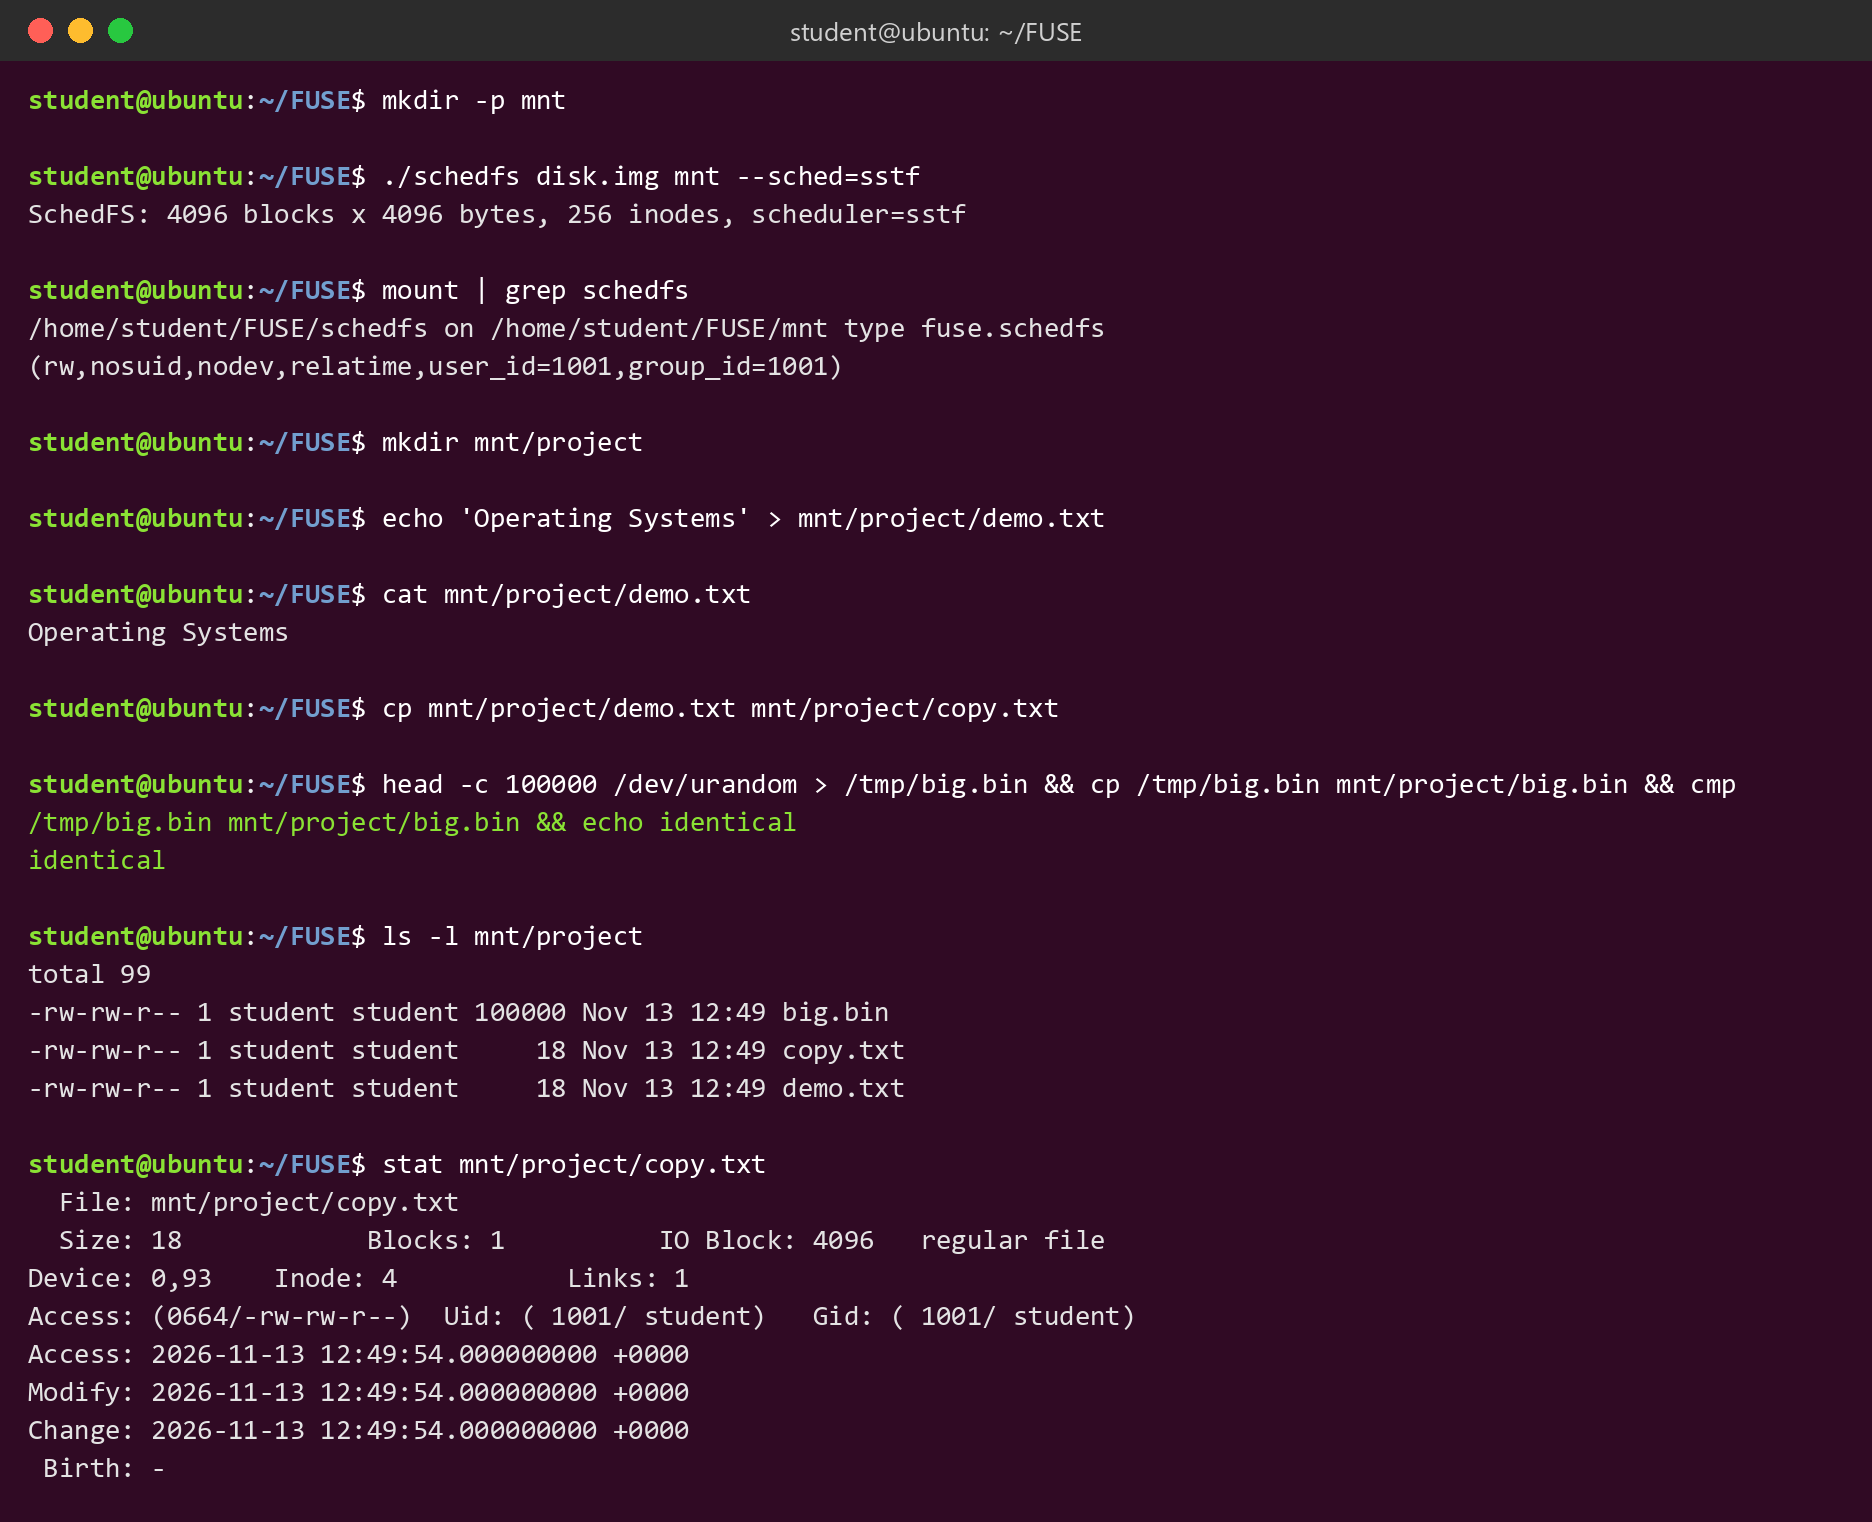
\includegraphics[width=\linewidth]{figures/screenshots/term_03_mount.png}
\caption{Mounting under SSTF and using the file system with ordinary commands.}
\label{fig:term-mount}
\end{figure}

\noindent In \figref{fig:term-mount} the kernel lists the mount as type \code{fuse.schedfs}. The 100{,}000-byte file needs 25 blocks, more than the 12 direct pointers, so it exercises the single-indirect block; \code{cmp} confirms that it reads back identical to the source.

\begin{figure}[H]
\centering
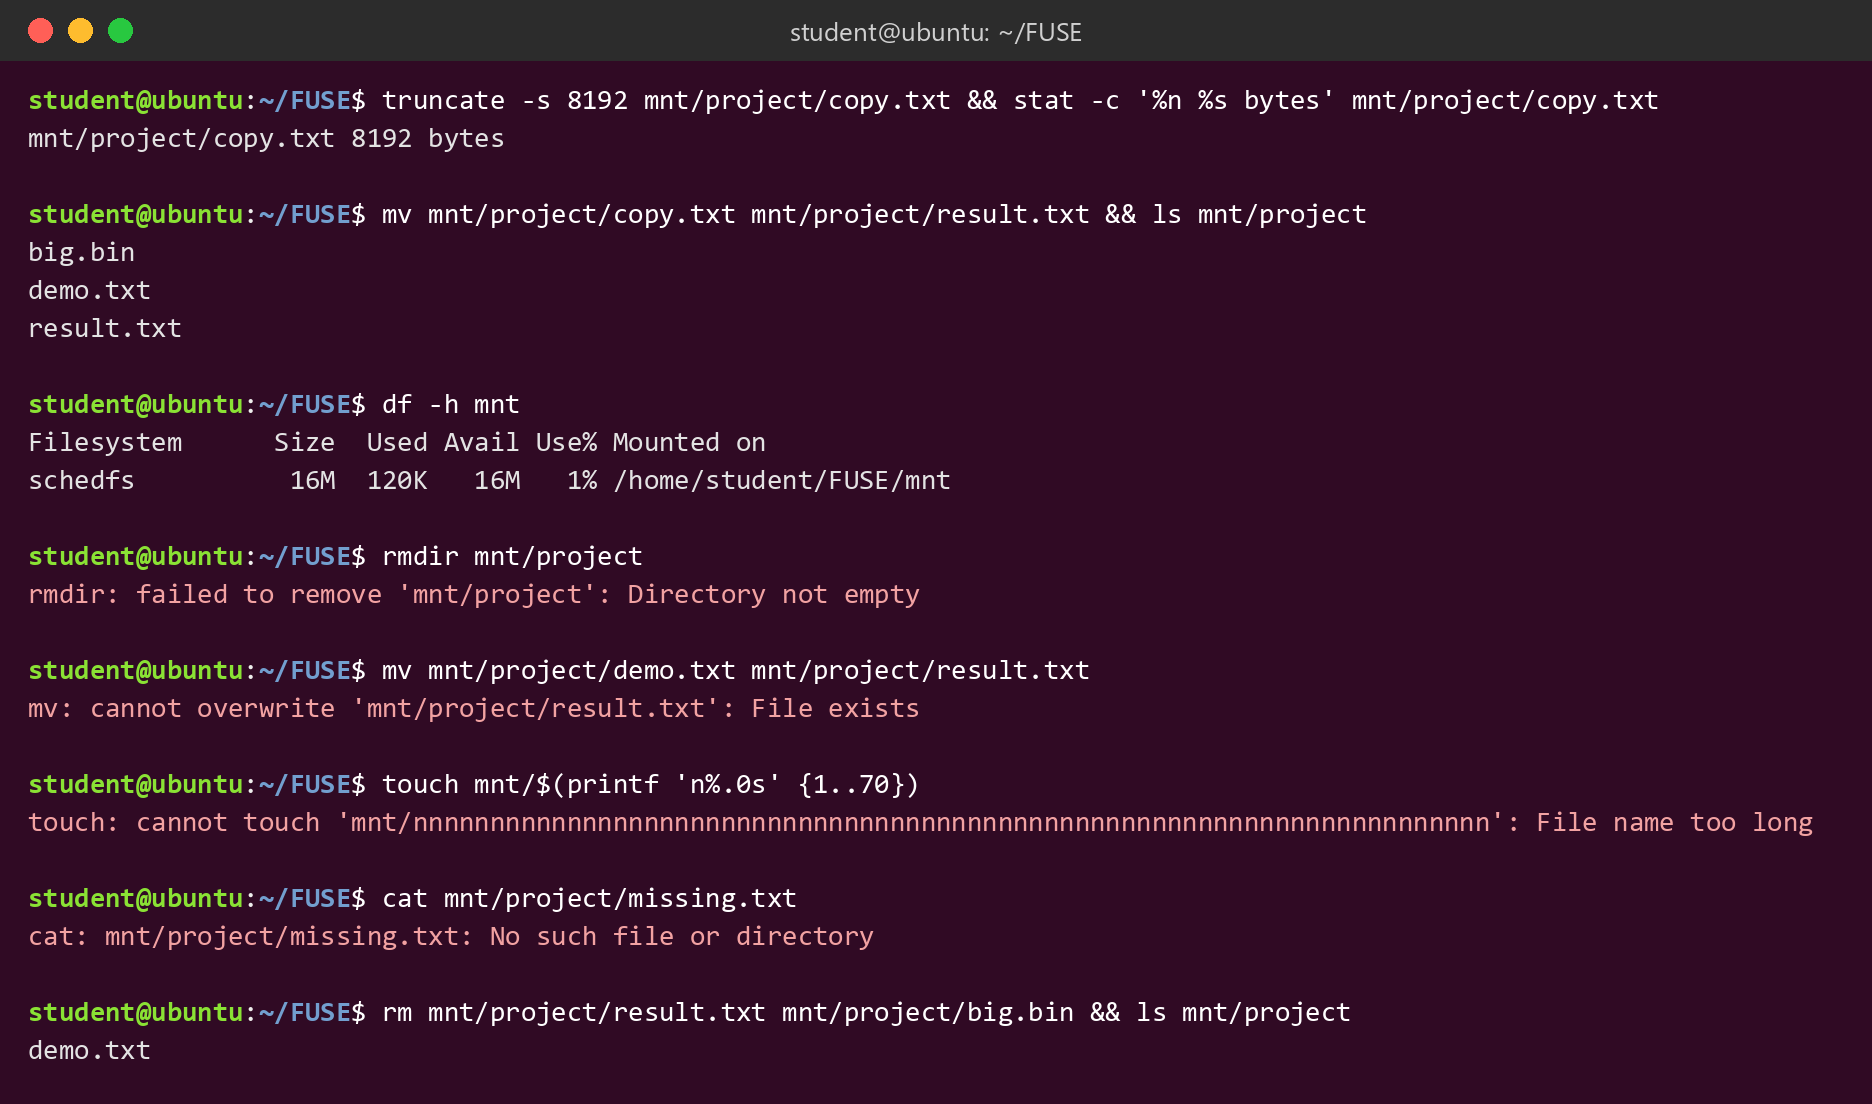
\includegraphics[width=\linewidth]{figures/screenshots/term_04_ops.png}
\caption{Truncate, rename, capacity reporting and error handling on the mounted file system.}
\label{fig:term-ops}
\end{figure}

\begin{figure}[H]
\centering
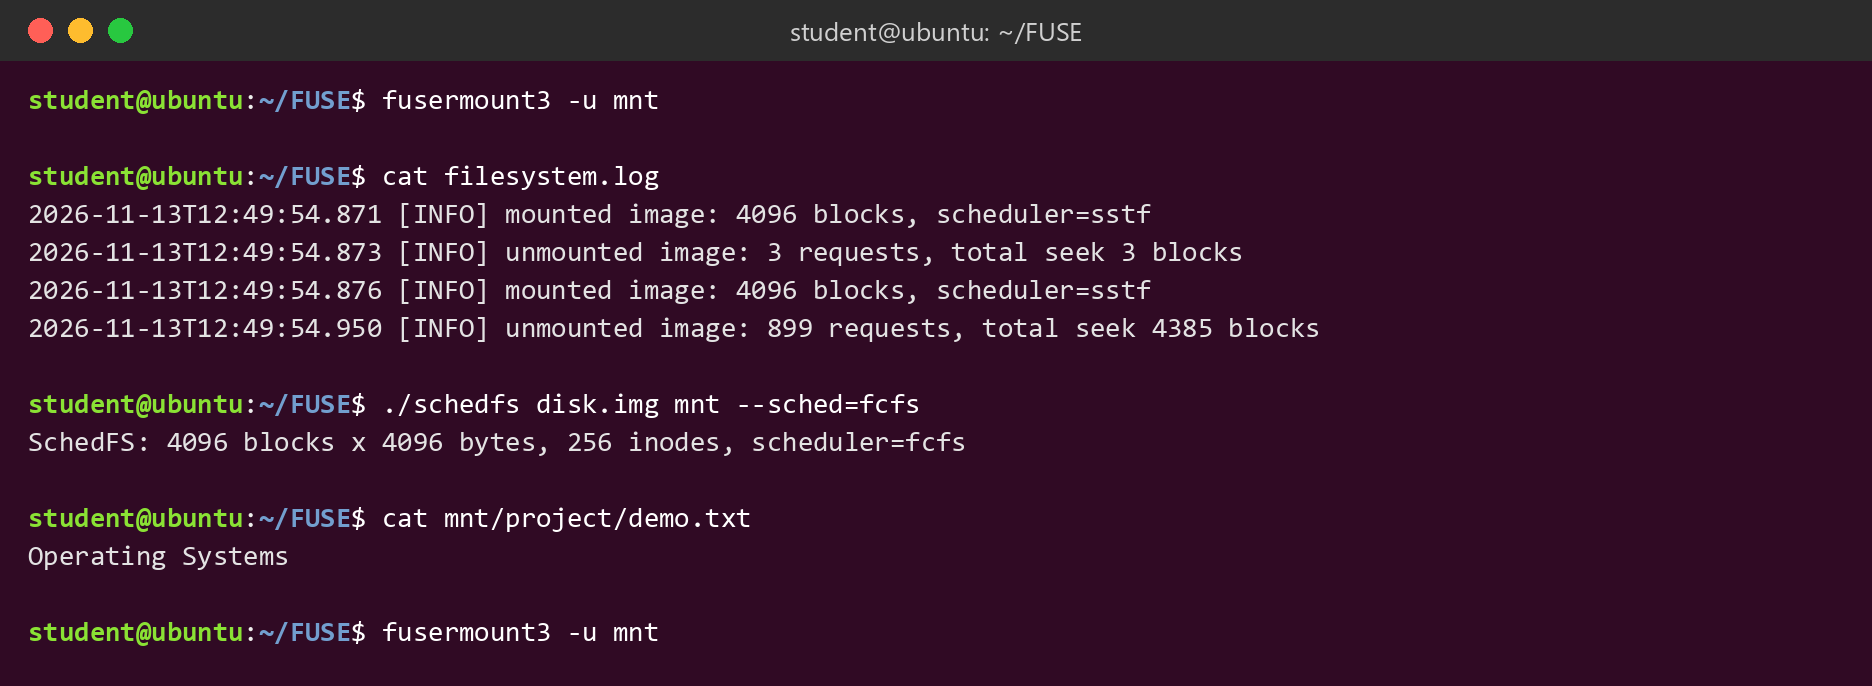
\includegraphics[width=\linewidth]{figures/screenshots/term_05_unmount.png}
\caption{Unmount summary in \code{filesystem.log}, and data persisting after a remount under FCFS.}
\label{fig:term-unmount}
\end{figure}

\noindent Each mount writes two log lines (\figref{fig:term-unmount}). The first pair, with 3 requests, comes from the validation mount in \code{main()}; the second pair is the real session, which served 899 block requests with a total head movement of 4{,}385 blocks.

\begin{figure}[H]
\centering
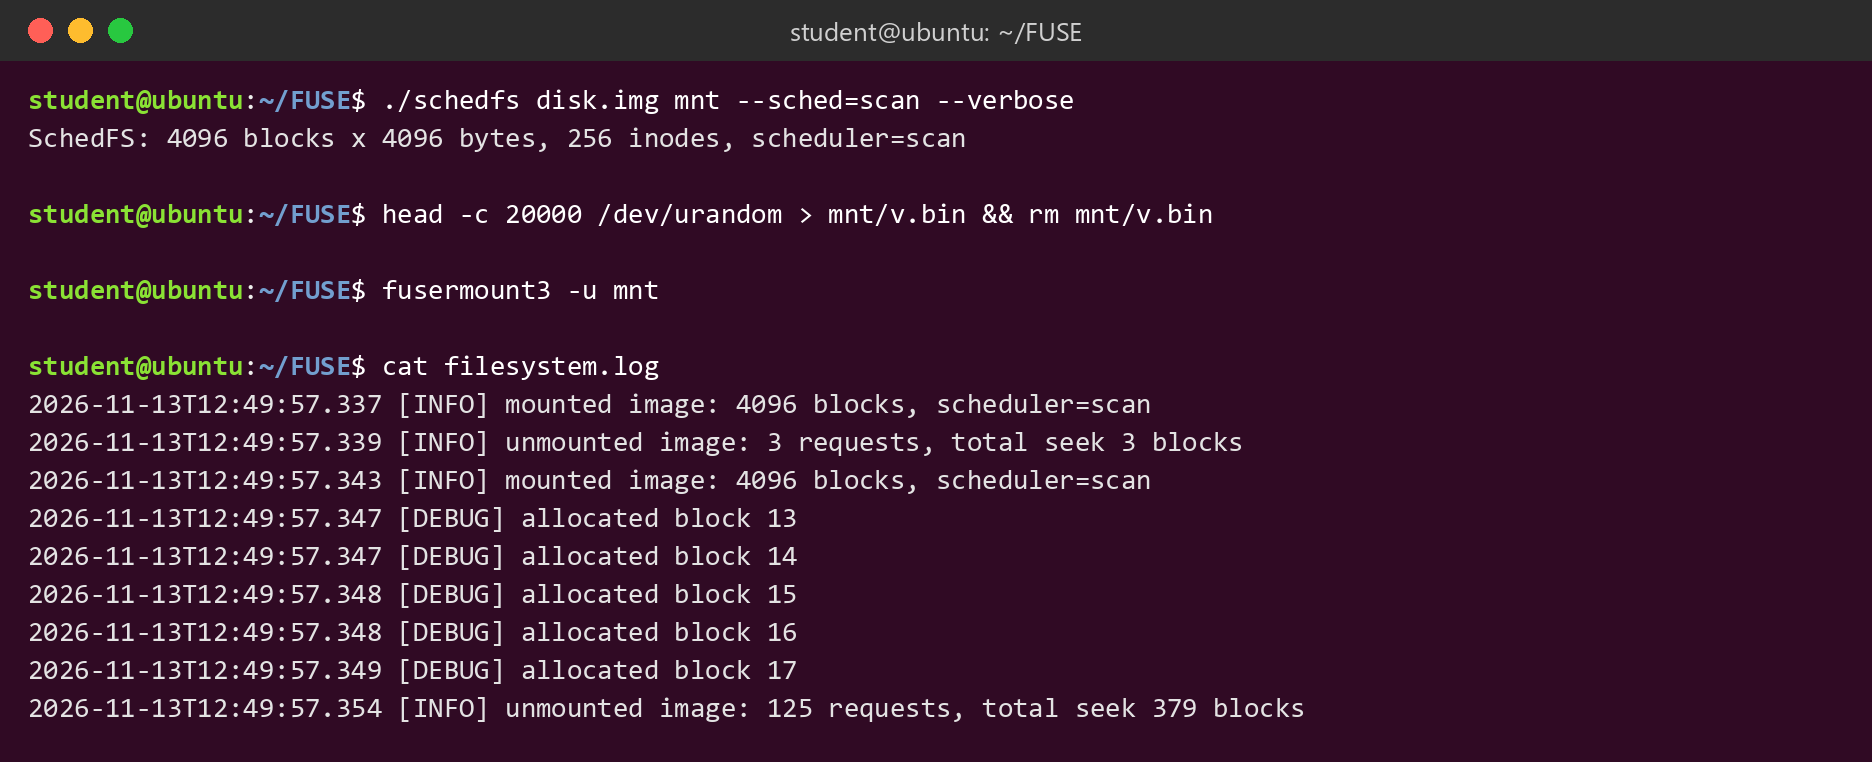
\includegraphics[width=\linewidth]{figures/screenshots/term_08_verbose.png}
\caption{Verbose mode under SCAN: DEBUG entries show five consecutive data blocks allocated for a 20{,}000-byte file.}
\label{fig:term-verbose}
\end{figure}

\noindent The allocations in \figref{fig:term-verbose} are consecutive (blocks 13--17) because of the hint-based allocator described in \figref{fig:fc-alloc}.

\begin{figure}[H]
\centering
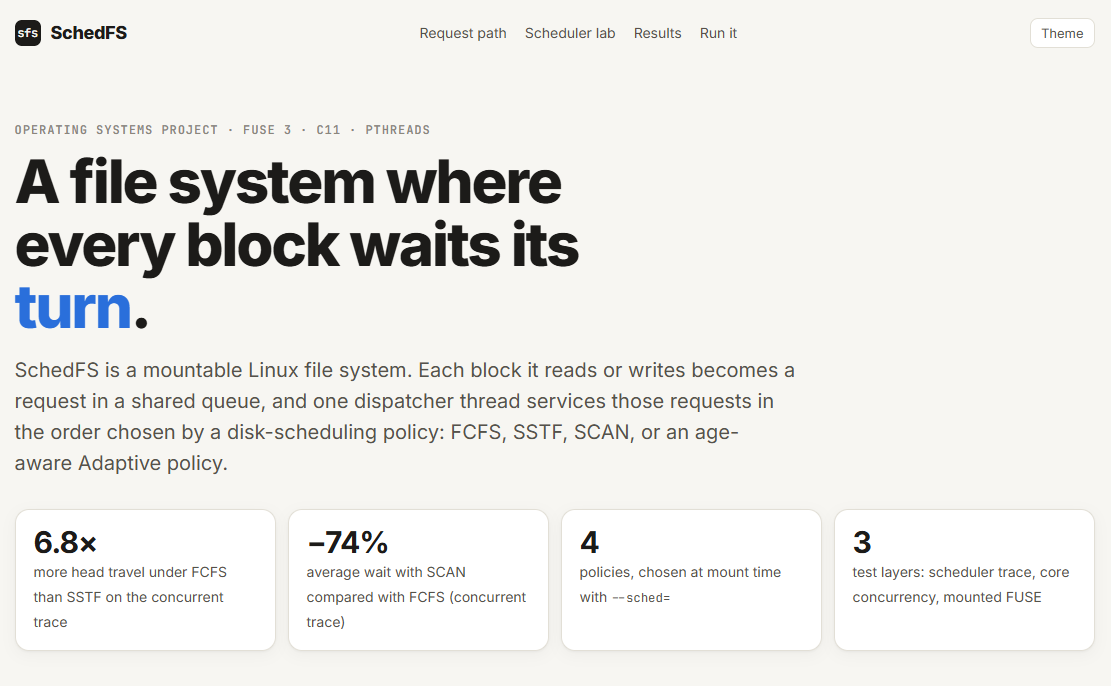
\includegraphics[width=0.86\linewidth]{figures/screenshots/web_hero.png}
\caption{Interactive demo page (GitHub Pages): overview of the project.}
\label{fig:web-hero}
\end{figure}

\begin{figure}[H]
\centering
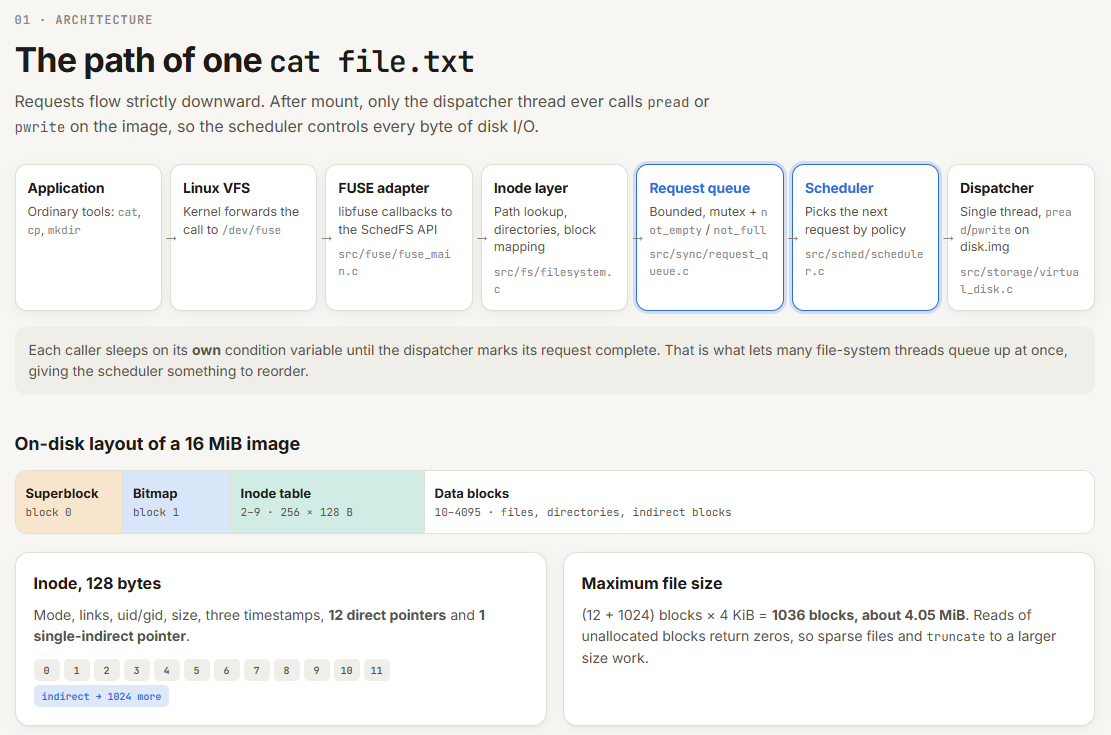
\includegraphics[width=0.86\linewidth]{figures/screenshots/web_request_path.png}
\caption{Demo page: the request path and the on-disk layout, linked to the source files.}
\label{fig:web-path}
\end{figure}

\begin{figure}[H]
\centering
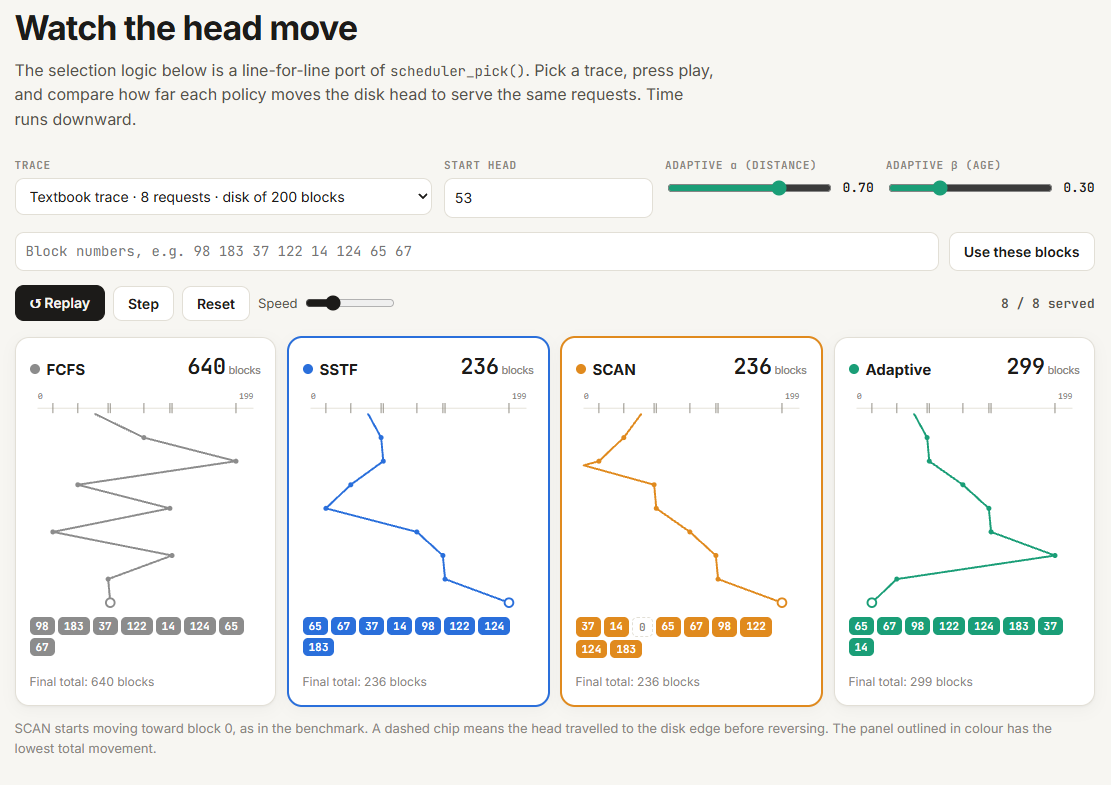
\includegraphics[width=0.86\linewidth]{figures/screenshots/web_lab_textbook.png}
\caption{Scheduler lab after playing the textbook trace: FCFS 640, SSTF 236, SCAN 236 and Adaptive 299 blocks.}
\label{fig:web-lab}
\end{figure}

\noindent The lab in \figref{fig:web-lab} runs a JavaScript port of \code{scheduler_pick()}. Its FCFS, SSTF and SCAN totals and service orders match the C unit test exactly. Its Adaptive total (299) uses a modelled clock in the browser, so it is shown for illustration only and is not one of the tested values.

\begin{figure}[H]
\centering
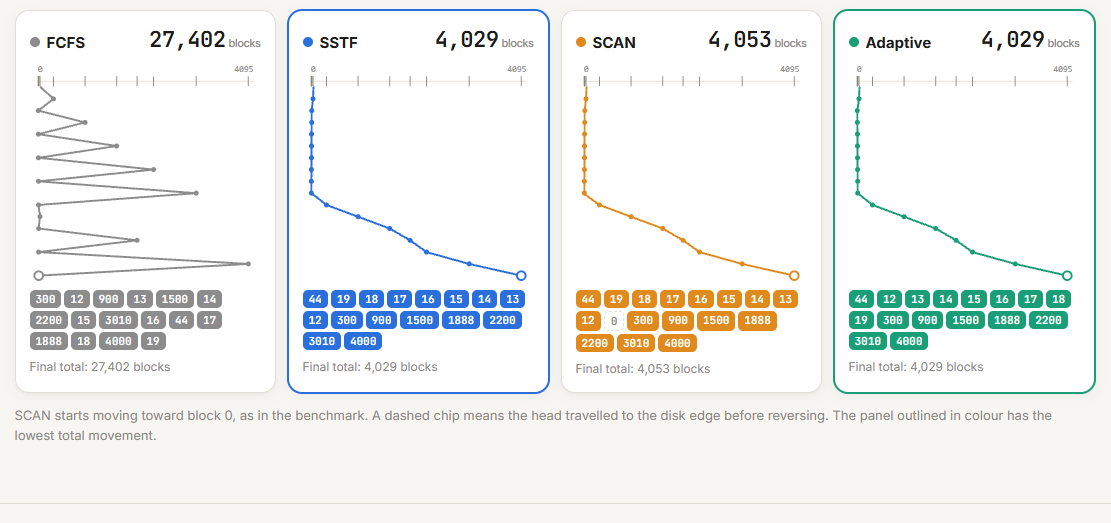
\includegraphics[width=0.86\linewidth]{figures/screenshots/web_lab_concurrent.png}
\caption{Scheduler lab on the 16-request concurrent trace: FCFS zig-zags across the disk (27{,}402 blocks).}
\label{fig:web-lab-conc}
\end{figure}

\begin{figure}[H]
\centering
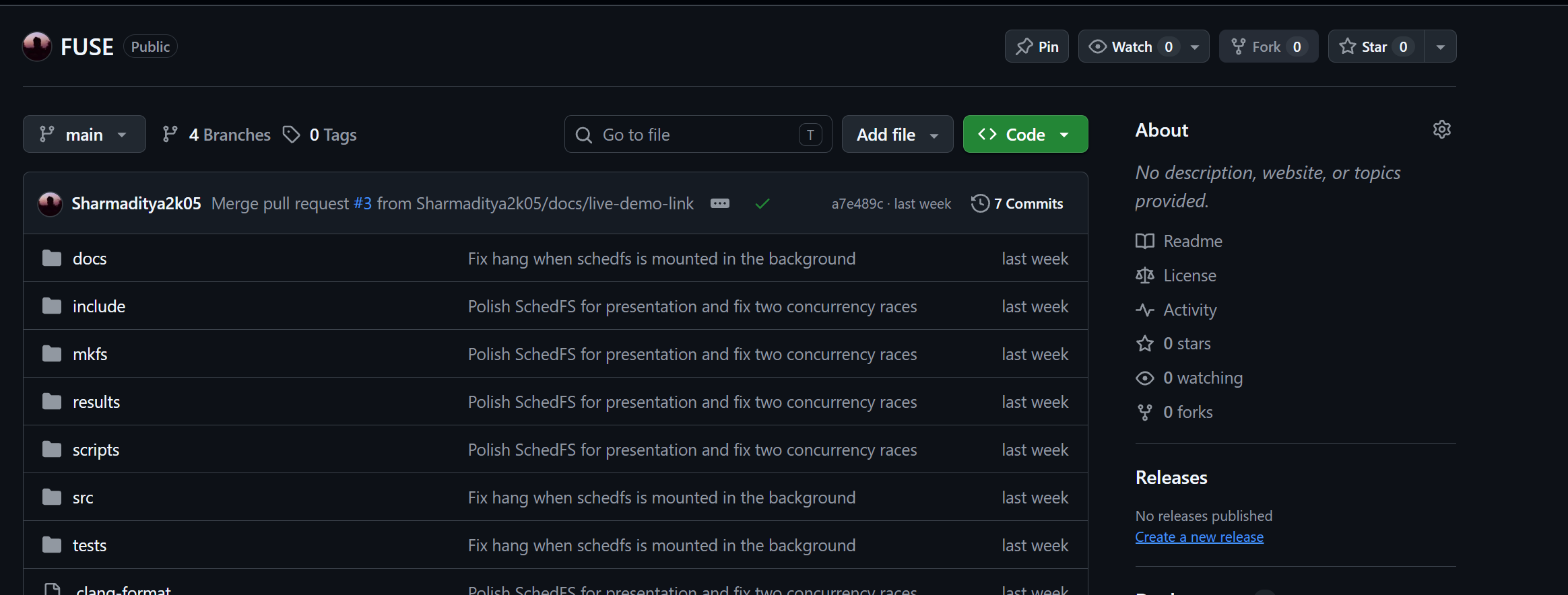
\includegraphics[width=\linewidth]{figures/screenshots/github_repo.png}
\caption{Repository on GitHub, with the merged pull requests and the \code{github-pages} deployment.}
\label{fig:github}
\end{figure}

% =====================================================================
\clearpage
\section{TESTING DETAILS}
\label{sec:testing}
% =====================================================================

\subsection{Testing Methodology}
Testing was carried out at the levels shown in \tabref{tab:levels}. Each level adds a layer of the real system: the scheduler alone, then the core file-system API with threads but without FUSE, then the mounted file system driven by shell commands, and finally measurement.

\begin{table}[H]
\centering
\caption{Testing levels and tools}
\label{tab:levels}
\small
\begin{tabularx}{\linewidth}{@{}l X l@{}}
\toprule
\textbf{Level} & \textbf{What is checked} & \textbf{Tool} \\
\midrule
Unit & exact service order and head movement of FCFS, SSTF, SCAN & \code{tests/test_scheduler.c} \\
Integration & create, write, read, truncate, sparse reads, persistence across remount, 4 concurrent writers & \code{tests/test_core.c} \\
System & a real FUSE mount under each policy, and in background mode, driven by \code{mkdir}, \code{cp}, \code{cmp}, \code{truncate}, \code{mv}, \code{rm}, \code{rmdir} & \code{tests/system.sh} \\
Functional & each functional requirement on a manually mounted image & shell session (\figref{fig:term-mount}--\figref{fig:term-verbose}) \\
Boundary & name length limit, file larger than the direct blocks, invalid image sizes & shell session \\
Error handling & invalid options, missing or foreign image, non-empty directory, existing target & shell session (\figref{fig:term-errors}) \\
Concurrency & data races under 4 threads & ThreadSanitizer \cite{serebryany2009} \\
Performance & seek distance, waiting time and throughput per policy & \code{schedfs-bench}; mounted workload \\
\bottomrule
\end{tabularx}
\end{table}

\noindent\textbf{Environment.} Docker Desktop on Windows 11 running the \code{ubuntu:24.04} image, with GCC 13.3.0 and libfuse 3.14.0 (\figref{fig:term-build}). The container had \code{/dev/fuse} and the \code{SYS_ADMIN} capability, and all tests ran as an unprivileged user, because \code{system.sh} refuses to run as root.

\subsection{Test Cases}
\label{sec:testcases}
\tabref{tab:tests} lists 25 test cases, against the minimum of four ($1 \times 4$). The ``Actual output'' column quotes the captured output.

{\footnotesize
\setlength{\tabcolsep}{3.5pt}
\begin{longtable}{@{}p{0.85cm}p{2.25cm}p{1.2cm}p{1.85cm}p{2.25cm}p{2.3cm}p{2.35cm}p{1.0cm}@{}}
\caption{Test cases and results}\label{tab:tests}\\
\toprule
\textbf{ID} & \textbf{Objective} & \textbf{Module} & \textbf{Pre-\newline condition} & \textbf{Input} & \textbf{Expected output} & \textbf{Actual output} & \textbf{Result} \\
\midrule
\endfirsthead
\toprule
\textbf{ID} & \textbf{Objective} & \textbf{Module} & \textbf{Pre-\newline condition} & \textbf{Input} & \textbf{Expected output} & \textbf{Actual output} & \textbf{Result} \\
\midrule
\endhead
\midrule \multicolumn{8}{r}{\emph{continued on next page}} \\
\endfoot
\bottomrule
\endlastfoot
TC01 & FCFS service order and movement & M6 & none & head 53; textbook queue & order as queued; 640 & assertion holds; ``scheduler tests passed'' & Pass \\
TC02 & SSTF service order and movement & M6 & none & same trace & 65, 67, 37, 14, 98, 122, 124, 183; 236 & assertion holds & Pass \\
TC03 & SCAN service order and movement & M6 & direction $-1$ & same trace & 37, 14, 65, \ldots, 183; 236 & assertion holds & Pass \\
TC04 & Format a valid image & M1 & no \code{disk.img} & \code{disk.img 16M} & 4096 blocks, 256 inodes, data at 10 & ``Formatted disk.img: 4096 blocks, 256 inodes, data starts at block 10'' & Pass \\
TC05 & Never overwrite an image & M1 & \code{disk.img} exists & same command & error, exit 1 & ``open (\ldots): File exists'' & Pass \\
TC06 & Reject invalid sizes & M1 & none & \code{10K}, \code{64K} & size error, exit 2 & ``size must be a positive multiple of 4096 (M/MiB/G/GiB accepted)'' & Pass \\
TC07 & Mount and report geometry & M2 & formatted image & \code{--sched=sstf} & geometry printed; mount listed & ``scheduler=sstf''; type \code{fuse.schedfs} & Pass \\
TC08 & Create, write and read a file & M3 & mounted & \code{echo}, \code{cat} & ``Operating Systems'' & ``Operating Systems'' & Pass \\
TC09 & Large file through indirect block & M3, M4 & mounted & 100{,}000 random bytes & identical copy & \code{cmp}: ``identical''; size 100000 & Pass \\
TC10 & Extend with \code{truncate} & M3, M4 & 18-byte file & \code{truncate -s 8192} & size 8192 & ``8192 bytes'' & Pass \\
TC11 & Rename and delete & M3 & files exist & \code{mv}, \code{rm} & entries renamed, removed & listing shows only \code{demo.txt} & Pass \\
TC12 & Name length limit (boundary) & M3 & mounted & 70-character name & \code{ENAMETOOLONG} & ``File name too long'' & Pass \\
TC13 & Remove non-empty directory & M3 & directory has files & \code{rmdir} & \code{ENOTEMPTY} & ``Directory not empty'' & Pass \\
TC14 & Rename onto existing target & M3 & both files exist & \code{mv a b} & refused (documented limit) & ``cannot overwrite \ldots: File exists'' & Pass \\
TC15 & Read missing file & M3 & mounted & \code{cat missing.txt} & \code{ENOENT} & ``No such file or directory'' & Pass \\
TC16 & Invalid mount options & M2 & none & \code{--sched=lifo}; \code{--alpha=-1} & usage; weight error & usage text; ``alpha and beta must be non-negative'' & Pass \\
TC17 & Missing or foreign image & M2, M3 & none & \code{nosuch.img}; 1 MiB of zeros & clear error, exit 1 & ``No such file or directory''; ``Invalid argument'' & Pass \\
TC18 & Persistence across remount & M3, M7 & data written; unmounted & remount with FCFS & same content & ``Operating Systems'' & Pass \\
TC19 & Concurrent writers (integration) & M3--M7 & fresh image & 4 threads $\times$ 64 KiB & each file intact after remount & ``core persistence and concurrency tests passed'' & Pass \\
TC20 & No data races & M3--M7 & TSan build & \code{test_core} & no reports; exit 0 & no reports; ``exit status: 0'' & Pass \\
TC21 & Mounted tests, all policies & M1--M7 & \code{/dev/fuse} & \code{system.sh} & all steps succeed & ``FUSE system tests passed'' & Pass \\
TC22 & Background (daemon) mount & M2, M7 & no \code{-f} & relative image path & I/O works; data persists & part of TC21; passed & Pass \\
TC23 & Metrics and DEBUG log & M8 & \code{--verbose} & 20{,}000-byte write & unmount summary; allocations & ``allocated block 13'' \ldots\ ``125 requests, total seek 379 blocks'' & Pass \\
TC24 & Benchmark reproducibility & M6, M9 & committed CSV & \code{schedfs-bench --all} & FCFS, SSTF, SCAN seek totals unchanged & all 15 equal; Adaptive differs in 3 of 5 (clock-dependent) & Pass \\
TC25 & Policy effect on mounted FS & M5--M7 & same image per run & 4 writers + 4 readers, 3 trials & equal requests; SSTF $<$ FCFS & 4{,}927 requests each; SSTF $-40\,\%$ & Pass \\
\end{longtable}
}

\subsection{Testing Results}
\label{sec:results}
All 25 test cases passed. \tabref{tab:testsummary} groups them by level.

\begin{table}[H]
\centering
\caption{Summary of test results}
\label{tab:testsummary}
\small
\begin{tabular}{@{}l l c c c@{}}
\toprule
\textbf{Level} & \textbf{Test cases} & \textbf{Executed} & \textbf{Passed} & \textbf{Failed} \\
\midrule
Unit & TC01--TC03 & 3 & 3 & 0 \\
Functional and boundary & TC04--TC12, TC23 & 10 & 10 & 0 \\
Error handling & TC13--TC17 & 5 & 5 & 0 \\
Integration and concurrency & TC18--TC20 & 3 & 3 & 0 \\
System & TC21--TC22 & 2 & 2 & 0 \\
Performance & TC24--TC25 & 2 & 2 & 0 \\
\midrule
\textbf{Total} & & \textbf{25} & \textbf{25} & \textbf{0} \\
\bottomrule
\end{tabular}
\end{table}

\noindent\textbf{Observations and limitations found during testing.}
\begin{itemize}[leftmargin=1.4em]
  \item \code{make test} prints ``Ignoring invalid max threads value 4294967295 > max (100000)'' once per foreground mount (\figref{fig:term-tests}). This message comes from libfuse 3.14.0, which reports an uninitialised default when \code{fuse_main()} runs a multi-threaded loop. SchedFS does not set this value, and the message does not affect any test.
  \item The formatter does not accept a \code{K} suffix (TC06). The message lists the accepted suffixes, but it could be clearer for a size such as \code{64K}, which is a multiple of 4096.
  \item \code{rename} onto an existing name is refused rather than replacing the target (TC14). This is a documented limitation, not a crash.
  \item Timing columns depend on the machine. On the Linux run, SSTF and SCAN have almost the same average wait on the concurrent trace (1.35 and 1.37~ms), whereas the repository's committed CSV, recorded on another machine, ranks SCAN clearly best. Only the seek columns of FCFS, SSTF and SCAN are exactly repeatable.
\end{itemize}

\subsubsection{Benchmark results}
\tabref{tab:bench} reports the benchmark run captured in \figref{fig:term-bench}. \figref{fig:chart-seek} and \figref{fig:chart-wait} plot the same data.

\begin{table}[H]
\centering
\caption{Benchmark results (Linux run, \figref{fig:term-bench}); best seek per workload in bold}
\label{tab:bench}
\small
\begin{tabular}{@{}l l r r r r@{}}
\toprule
\textbf{Workload} & \textbf{Policy} & \makecell[r]{\textbf{Total seek}\\\textbf{(blocks)}} & \makecell[r]{\textbf{Avg. wait}\\\textbf{(ms)}} & \makecell[r]{\textbf{Max. wait}\\\textbf{(ms)}} & \makecell[r]{\textbf{Throughput}\\\textbf{(req/s)}} \\
\midrule
\multirow{4}{*}{Sequential (8)} & FCFS & 50 & 0.113 & 0.162 & 44{,}185 \\
 & SSTF & \textbf{43} & 0.102 & 0.165 & 45{,}078 \\
 & SCAN & \textbf{43} & 0.101 & 0.155 & 47{,}900 \\
 & Adaptive & 50 & 0.113 & 0.162 & 44{,}185 \\
\midrule
\multirow{4}{*}{Random (7)} & FCFS & 631 & 0.633 & 1.191 & 5{,}252 \\
 & SSTF & 295 & 0.265 & 0.629 & 10{,}589 \\
 & SCAN & \textbf{229} & 0.194 & 0.454 & 13{,}231 \\
 & Adaptive & 295 & 0.371 & 0.629 & 10{,}586 \\
\midrule
\multirow{4}{*}{Clustered (7)} & FCFS & \textbf{58} & 0.106 & 0.166 & 37{,}294 \\
 & SSTF & \textbf{58} & 0.106 & 0.165 & 37{,}455 \\
 & SCAN & 164 & 0.288 & 0.377 & 17{,}547 \\
 & Adaptive & \textbf{58} & 0.109 & 0.170 & 36{,}459 \\
\midrule
\multirow{4}{*}{Mixed (11)} & FCFS & 736 & 0.538 & 1.246 & 6{,}944 \\
 & SSTF & 237 & 0.190 & 0.510 & 18{,}595 \\
 & SCAN & 229 & 0.162 & 0.488 & 19{,}314 \\
 & Adaptive & \textbf{209} & 0.164 & 0.448 & 20{,}776 \\
\midrule
\multirow{4}{*}{Concurrent (16)} & FCFS & 27{,}402 & 18.923 & 46.986 & 291 \\
 & SSTF & \textbf{4{,}029} & 1.355 & 6.216 & 1{,}946 \\
 & SCAN & 4{,}053 & 1.373 & 6.265 & 1{,}935 \\
 & Adaptive & 4{,}523 & 2.216 & 7.205 & 1{,}737 \\
\bottomrule
\end{tabular}
\end{table}

\pgfplotsset{
  policybars/.style={
    ybar, bar width=5.5pt, width=\linewidth, height=6.4cm, enlarge x limits=0.12,
    symbolic x coords={Sequential,Random,Clustered,Mixed,Concurrent}, xtick=data,
    tick label style={font=\scriptsize}, label style={font=\small},
    legend style={font=\scriptsize, at={(0.5,1.03)}, anchor=south, legend columns=4, draw=none},
    ymajorgrids, grid style={gray!25}, log origin=infty},
}
\begin{figure}[H]
\centering
\begin{tikzpicture}
\begin{axis}[policybars, ymode=log, ymin=20, ymax=60000, ylabel={total seek (blocks, log scale)}]
  \addplot[fill=gray!60, draw=gray!80!black] coordinates {(Sequential,50) (Random,631) (Clustered,58) (Mixed,736) (Concurrent,27402)};
  \addplot[fill=blue!55, draw=blue!70!black] coordinates {(Sequential,43) (Random,295) (Clustered,58) (Mixed,237) (Concurrent,4029)};
  \addplot[fill=orange!70, draw=orange!80!black] coordinates {(Sequential,43) (Random,229) (Clustered,164) (Mixed,229) (Concurrent,4053)};
  \addplot[fill=teal!55, draw=teal!70!black] coordinates {(Sequential,50) (Random,295) (Clustered,58) (Mixed,209) (Concurrent,4523)};
  \legend{FCFS, SSTF, SCAN, Adaptive}
\end{axis}
\end{tikzpicture}
\caption{Total seek distance per workload and policy (lower is better).}
\label{fig:chart-seek}
\end{figure}

\begin{figure}[H]
\centering
\begin{tikzpicture}
\begin{axis}[policybars, ymode=log, ymin=0.05, ymax=60, ylabel={average wait (ms, log scale)}]
  \addplot[fill=gray!60, draw=gray!80!black] coordinates {(Sequential,0.112635) (Random,0.632521) (Clustered,0.106215) (Mixed,0.537896) (Concurrent,18.92333)};
  \addplot[fill=blue!55, draw=blue!70!black] coordinates {(Sequential,0.102348) (Random,0.264811) (Clustered,0.105727) (Mixed,0.190065) (Concurrent,1.354655)};
  \addplot[fill=orange!70, draw=orange!80!black] coordinates {(Sequential,0.101206) (Random,0.193812) (Clustered,0.287521) (Mixed,0.162019) (Concurrent,1.37267)};
  \addplot[fill=teal!55, draw=teal!70!black] coordinates {(Sequential,0.11254) (Random,0.371026) (Clustered,0.109257) (Mixed,0.163968) (Concurrent,2.215624)};
  \legend{FCFS, SSTF, SCAN, Adaptive}
\end{axis}
\end{tikzpicture}
\caption{Average waiting time per workload and policy (lower is better).}
\label{fig:chart-wait}
\end{figure}

\noindent\textbf{Analysis.}
\begin{itemize}[leftmargin=1.4em]
  \item \emph{Contention favours position-aware policies.} On the concurrent trace FCFS moves the head 27{,}402 blocks against 4{,}029 for SSTF, which is 6.8 times as far, and its average wait is about 14 times longer (18.9 against 1.35~ms).
  \item \emph{No policy wins everywhere.} SCAN is best on the random trace (229) but worst on the clustered trace (164 against 58), because it travels to the disk edge even when every request is nearby.
  \item \emph{The Adaptive policy depends on timing.} On the mixed trace it beat every other policy in this run (209), while the committed CSV recorded 237. Its score uses measured waiting times, so small timing differences change its choices. This is the expected cost of ageing based on real time.
\end{itemize}

\subsubsection{Scheduling on the mounted file system}
The benchmark isolates the scheduler. To measure the policies on real file-system traffic, the same workload was run on a fresh copy of one image under each policy, three times each (\figref{fig:term-policies}). Four background \code{head} processes each wrote 256~KiB at the same time, four \code{cat} processes then read the files back, and the files were deleted. Every run served exactly 4{,}927 block requests, so only the \emph{order} of service differed. \tabref{tab:mounted} and \figref{fig:chart-mounted} summarise the results.

\begin{table}[H]
\centering
\caption{Total head movement on the mounted file system (4{,}927 requests per run)}
\label{tab:mounted}
\small
\begin{tabular}{@{}l r r r r r r@{}}
\toprule
\textbf{Policy} & \textbf{Trial 1} & \textbf{Trial 2} & \textbf{Trial 3} & \textbf{Mean} & \textbf{Per request} & \textbf{vs. FCFS} \\
\midrule
FCFS & 199{,}289 & 195{,}909 & 186{,}121 & 193{,}773 & 39.3 & --- \\
SSTF & 117{,}041 & 112{,}565 & 118{,}935 & \textbf{116{,}180} & \textbf{23.6} & $-40.0$\,\% \\
SCAN & 126{,}521 & 134{,}431 & 136{,}659 & 132{,}537 & 26.9 & $-31.6$\,\% \\
Adaptive & 184{,}475 & 179{,}565 & 195{,}087 & 186{,}376 & 37.8 & $-3.8$\,\% \\
\bottomrule
\end{tabular}
\end{table}

\begin{figure}[H]
\centering
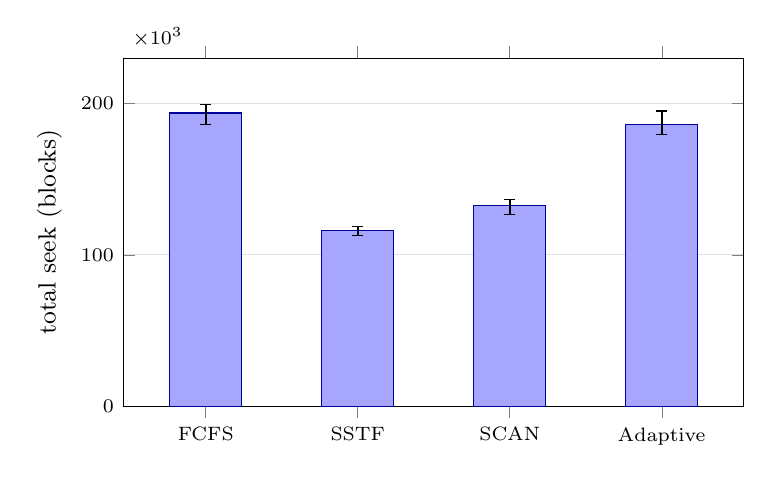
\begin{tikzpicture}
\begin{axis}[ybar, bar width=26pt, width=0.78\linewidth, height=6cm,
    symbolic x coords={FCFS,SSTF,SCAN,Adaptive}, xtick=data, ymin=0, ymax=230000,
    ylabel={total seek (blocks)}, tick label style={font=\scriptsize}, label style={font=\small},
    scaled y ticks=base 10:-3, ytick scale label code/.code={\scriptsize$\times 10^{3}$},
    ymajorgrids, grid style={gray!25}, enlarge x limits=0.18]
  \addplot[fill=blue!35, draw=blue!60!black,
           error bars/.cd, y dir=both, y explicit, error bar style={thick, black}]
    coordinates {
      (FCFS,193773) += (0,5516) -= (0,7652)
      (SSTF,116180) += (0,2755) -= (0,3615)
      (SCAN,132537) += (0,4122) -= (0,6016)
      (Adaptive,186376) += (0,8711) -= (0,6811)};
\end{axis}
\end{tikzpicture}
\caption{Mean total seek on the mounted file system; error bars show the minimum and maximum of three trials.}
\label{fig:chart-mounted}
\end{figure}

\noindent The ranking on real traffic is SSTF, then SCAN, then Adaptive, then FCFS, and the spread between trials is small compared with the differences between policies. The Adaptive policy behaves almost like FCFS here, and its score explains why. The distance term is normalised by the disk size, 4{,}096 blocks. Requests on this small image are rarely more than a few hundred blocks apart, so $\alpha \cdot d/N$ stays below about $0.05$, while $\beta \cdot w/w_{\max}$ ranges up to $0.3$. The age term dominates, and the policy serves requests roughly in arrival order. Lowering $\beta$ or normalising distance by the span of the pending requests would move it towards SSTF. This is a design improvement identified by testing.

\subsection{Testing Screenshots}
\label{sec:testshots}

\begin{figure}[H]
\centering
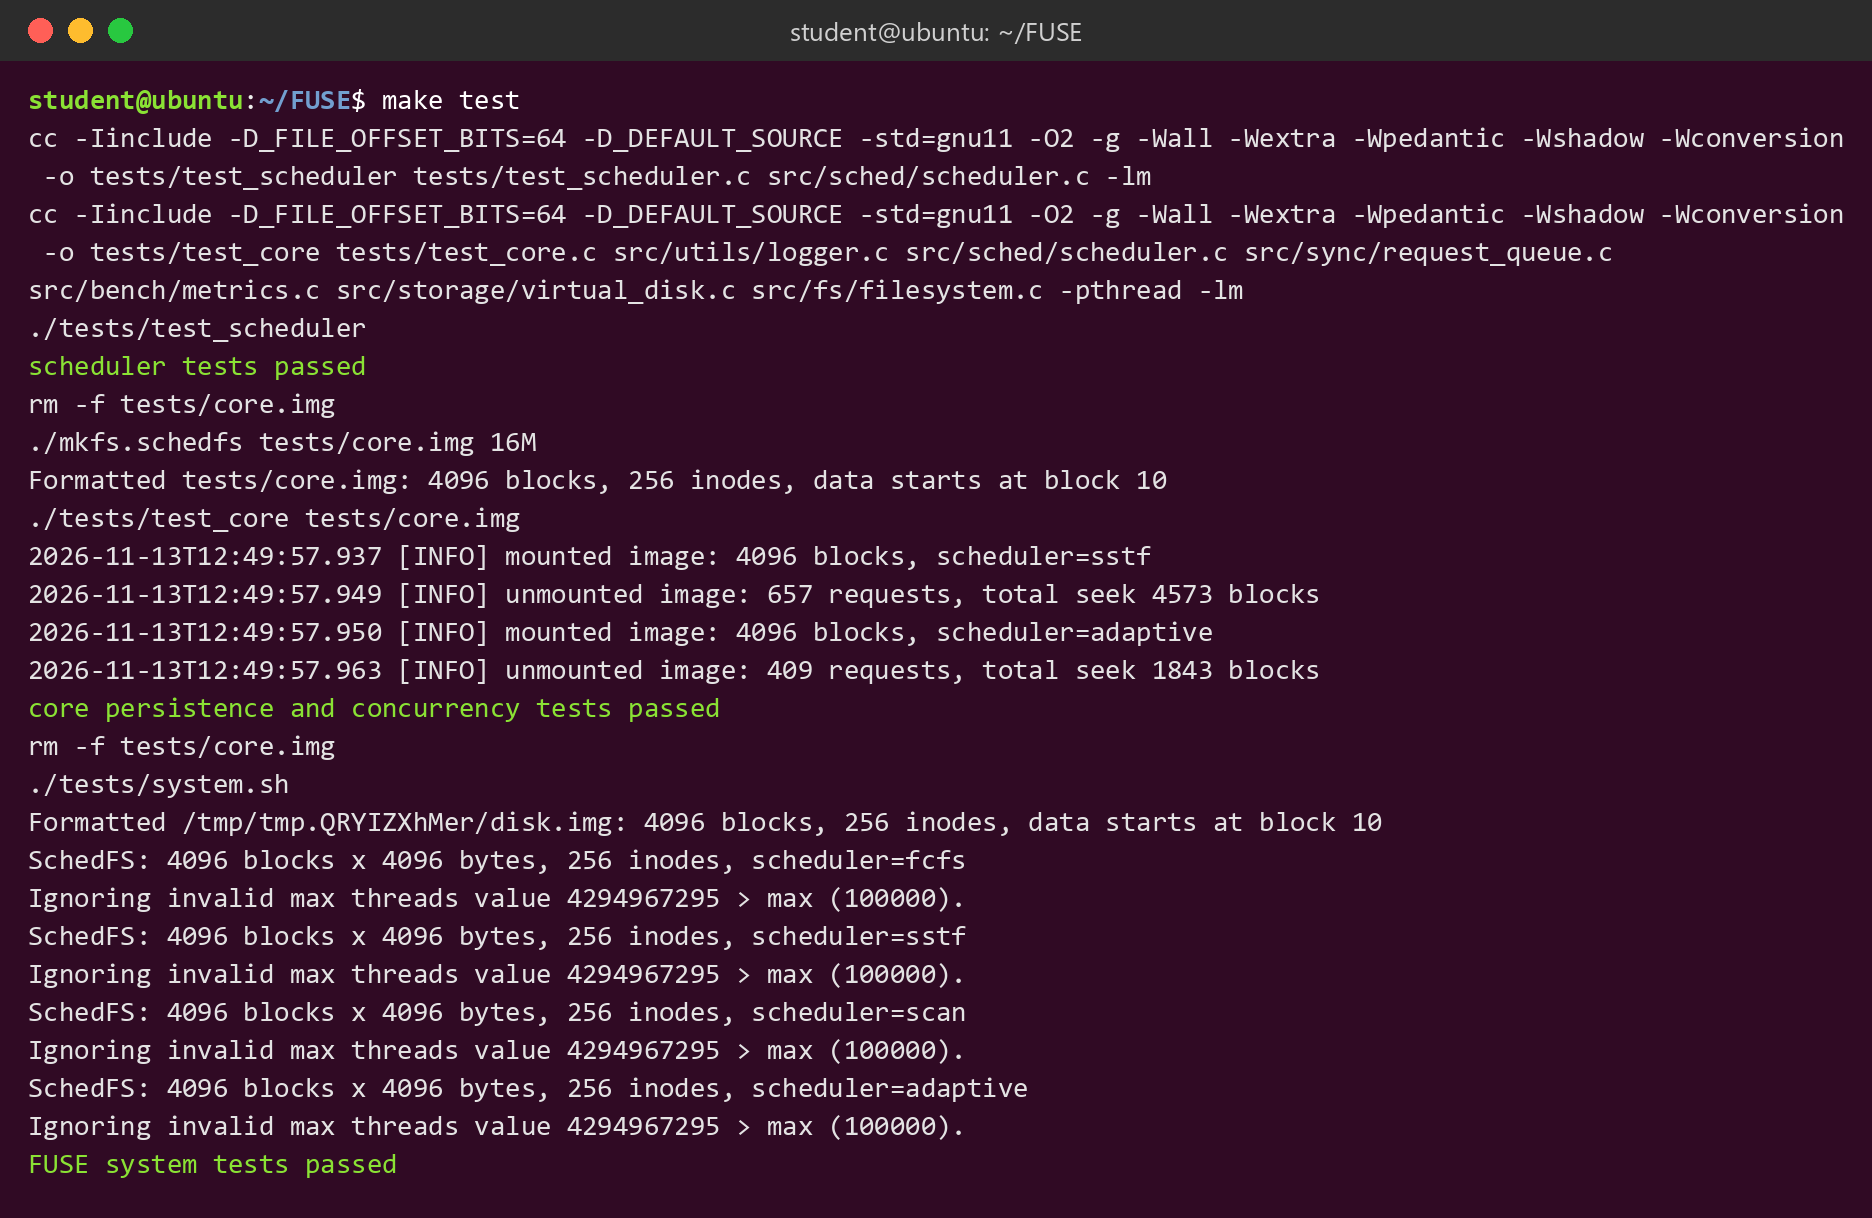
\includegraphics[width=\linewidth]{figures/screenshots/term_09_tests.png}
\caption{\code{make test}: scheduler unit test, core persistence and concurrency test, and mounted system tests under all four policies, all passing (TC01--TC03, TC19, TC21, TC22).}
\label{fig:term-tests}
\end{figure}

\begin{figure}[H]
\centering
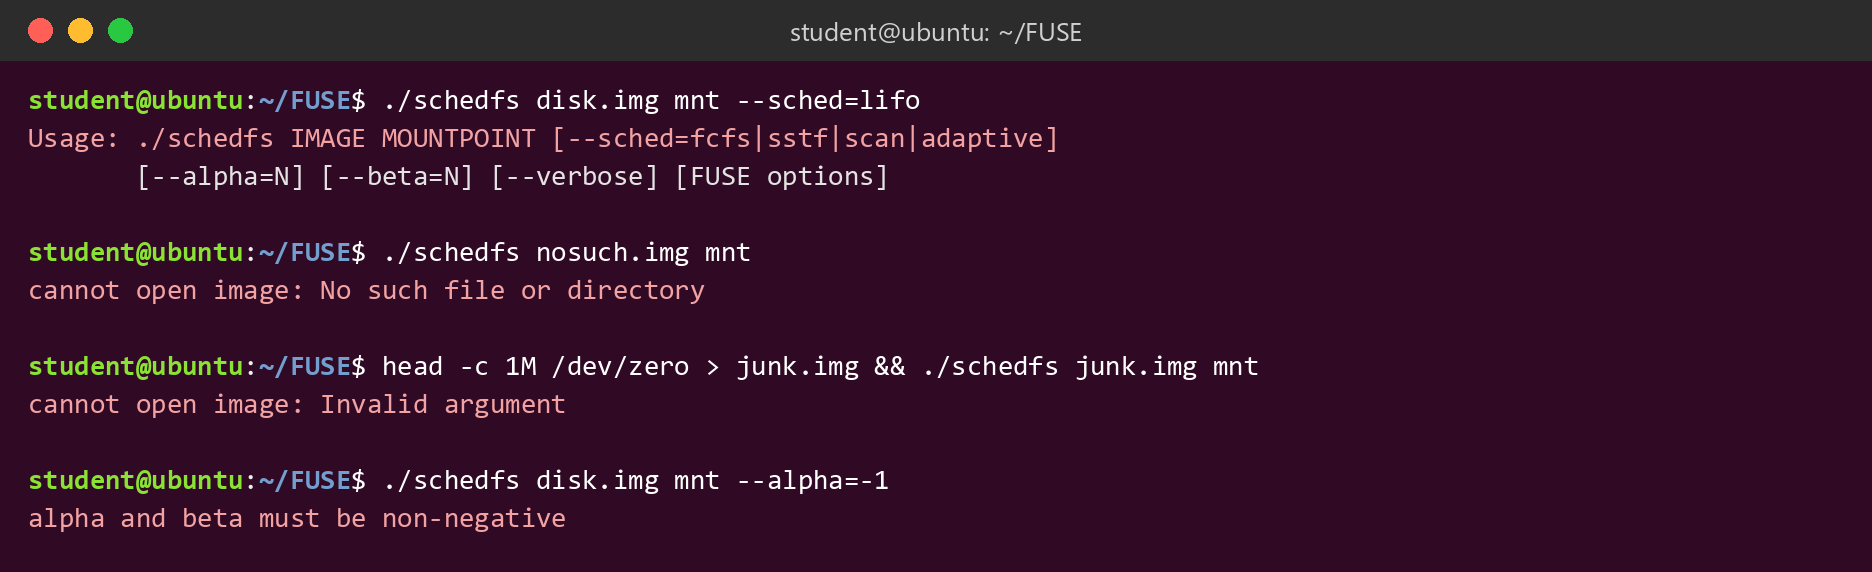
\includegraphics[width=\linewidth]{figures/screenshots/term_06_errors.png}
\caption{Error handling at mount time: unknown policy, missing image, non-SchedFS image and negative weight (TC16, TC17).}
\label{fig:term-errors}
\end{figure}

\begin{figure}[H]
\centering
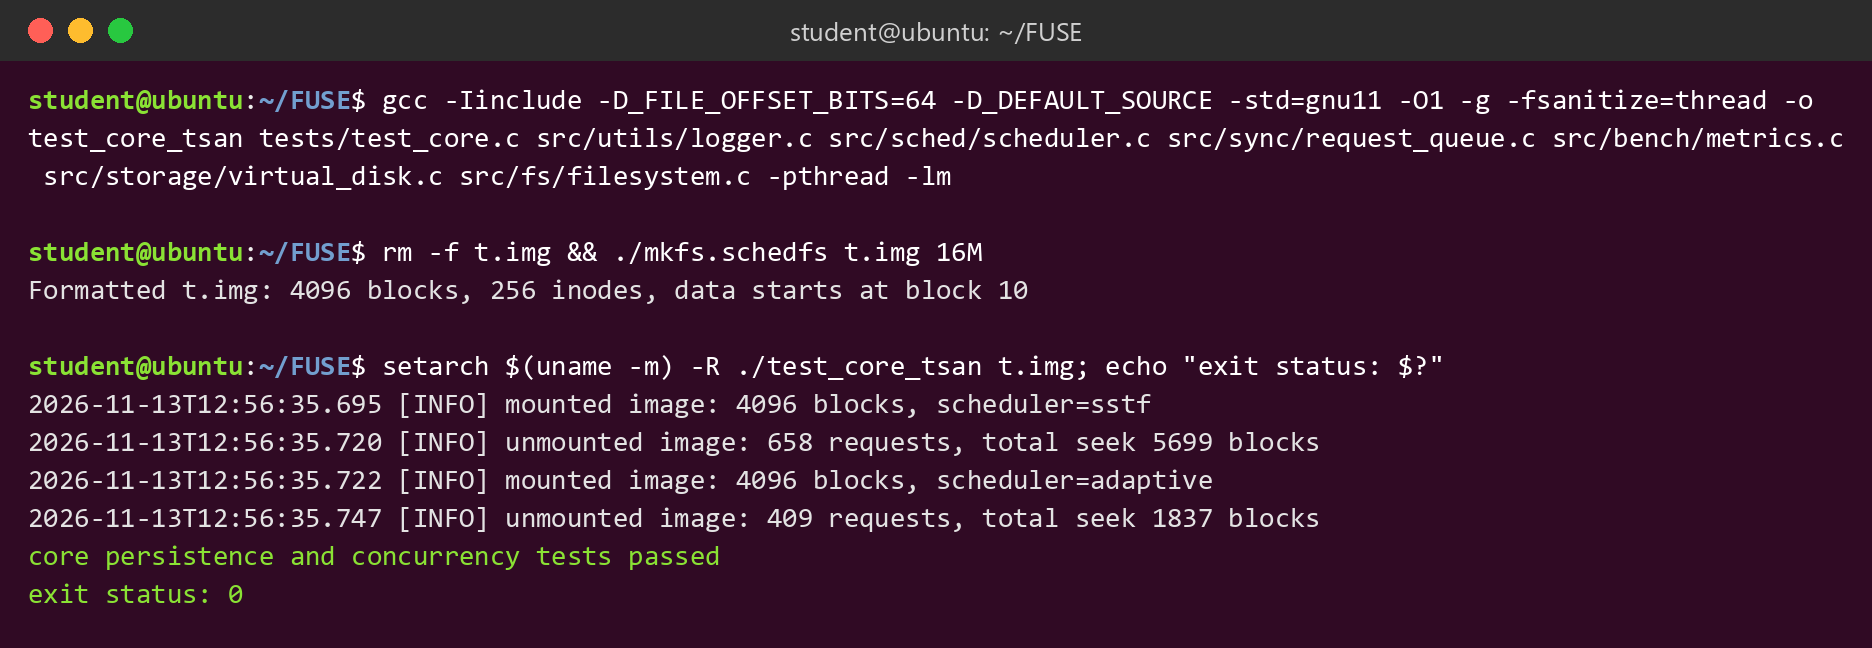
\includegraphics[width=\linewidth]{figures/screenshots/term_11_tsan.png}
\caption{ThreadSanitizer build of the core concurrency test: no data races reported, exit status 0 (TC20).}
\label{fig:term-tsan}
\end{figure}

\begin{figure}[H]
\centering
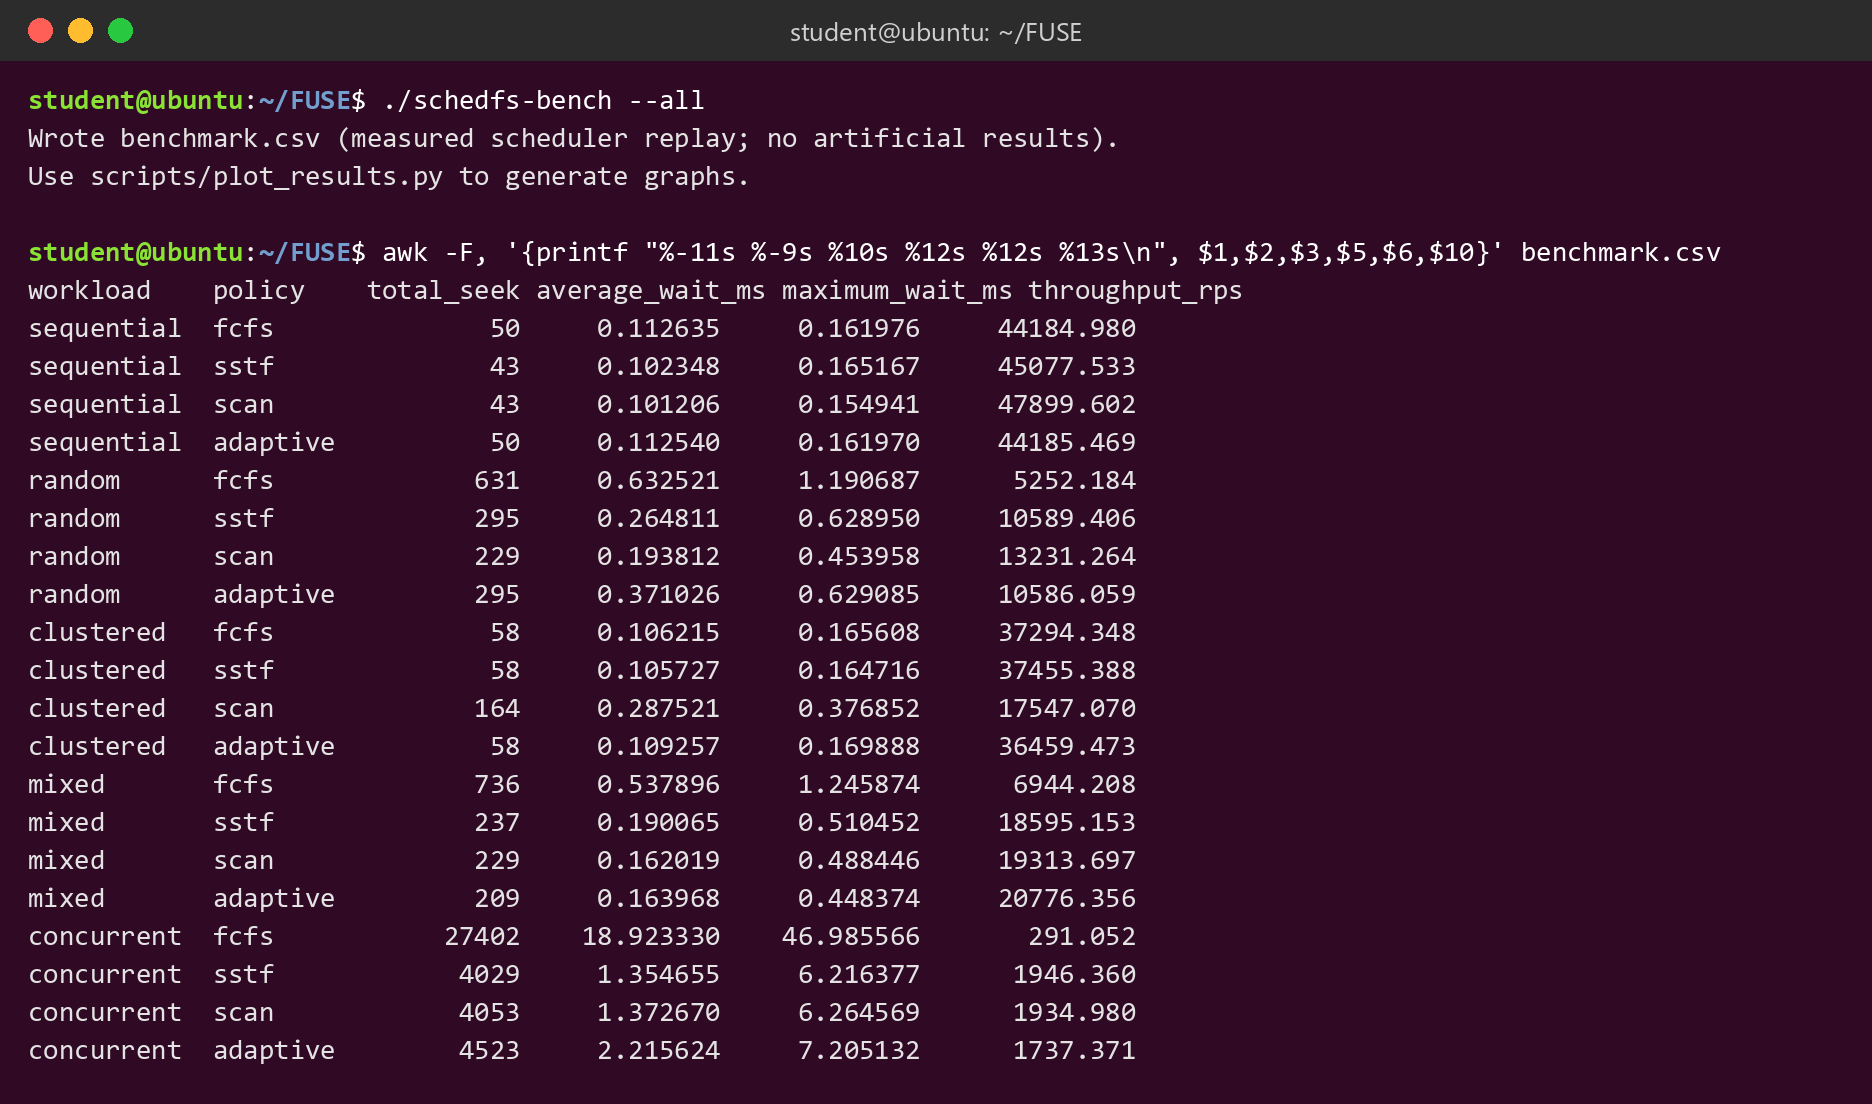
\includegraphics[width=\linewidth]{figures/screenshots/term_10_bench.png}
\caption{Benchmark run and its CSV output (TC24; data in \tabref{tab:bench}).}
\label{fig:term-bench}
\end{figure}

\begin{figure}[H]
\centering
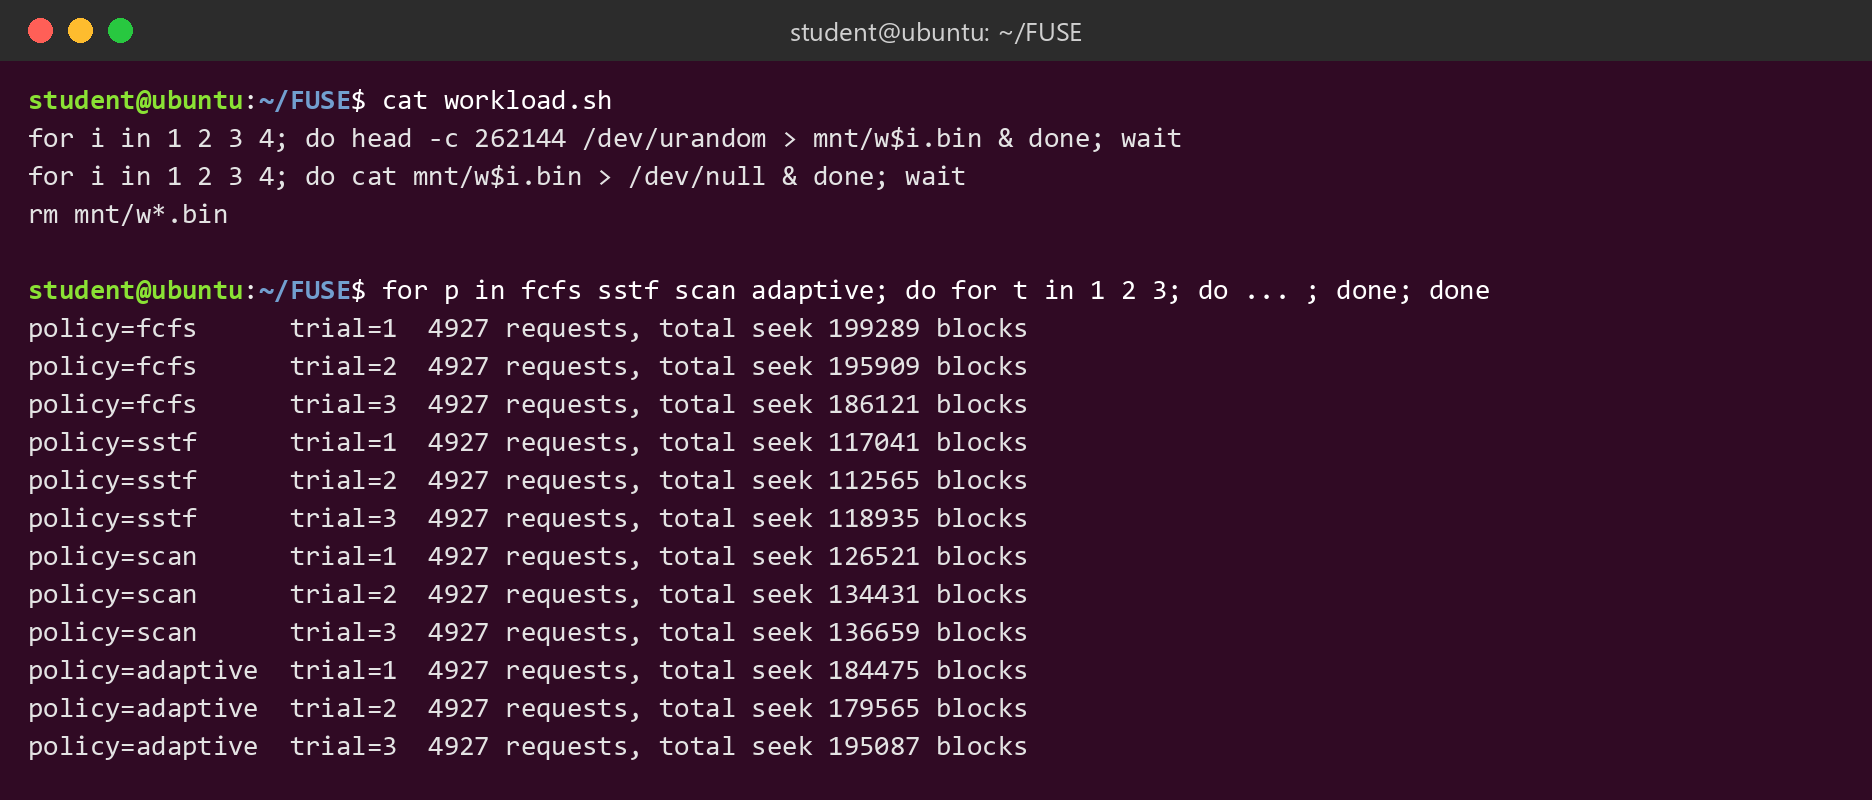
\includegraphics[width=\linewidth]{figures/screenshots/term_07_policies.png}
\caption{The same mounted workload under each policy, three trials each (TC25; data in \tabref{tab:mounted}).}
\label{fig:term-policies}
\end{figure}

\begin{figure}[H]
\centering
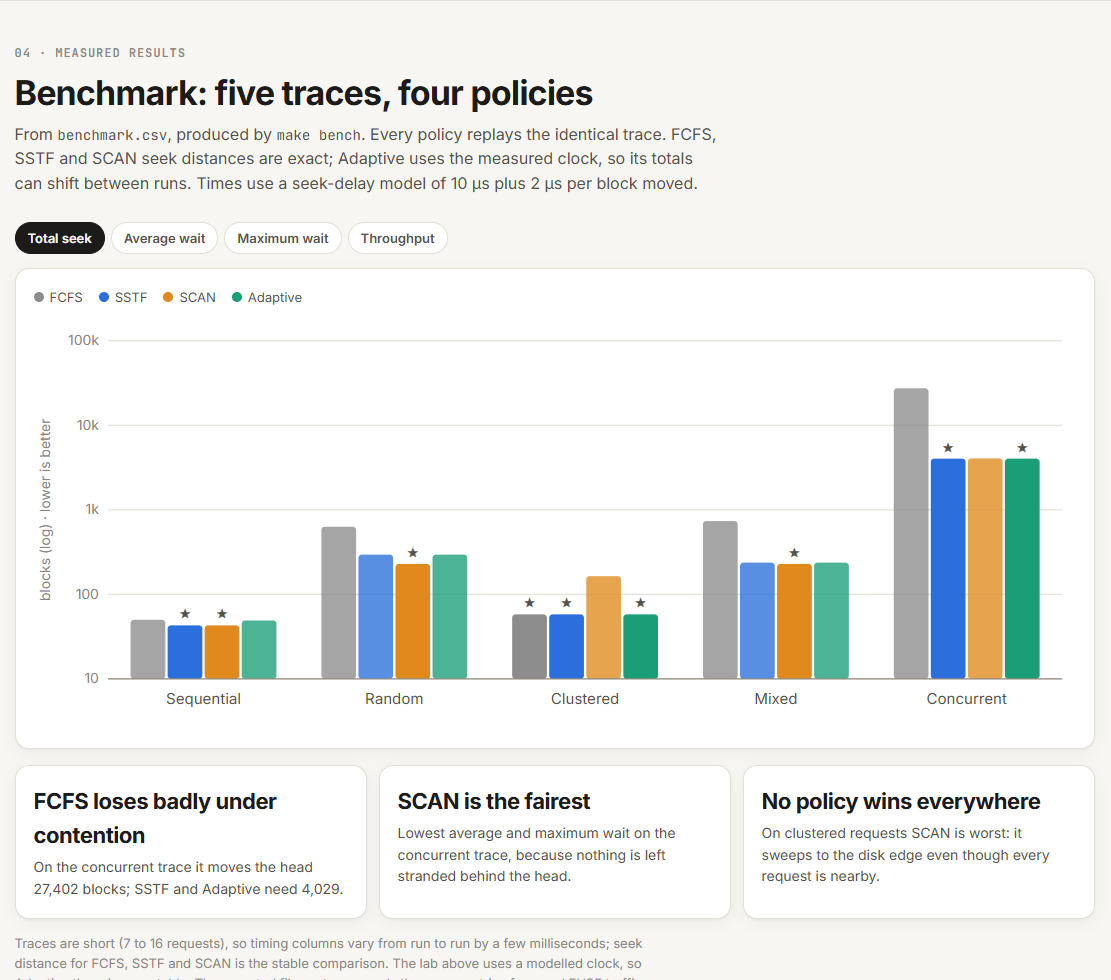
\includegraphics[width=0.86\linewidth]{figures/screenshots/web_benchmark_chart.png}
\caption{Benchmark view of the demo page, drawn from the repository's committed \code{benchmark.csv}.}
\label{fig:web-bench}
\end{figure}

\begin{figure}[H]
\centering
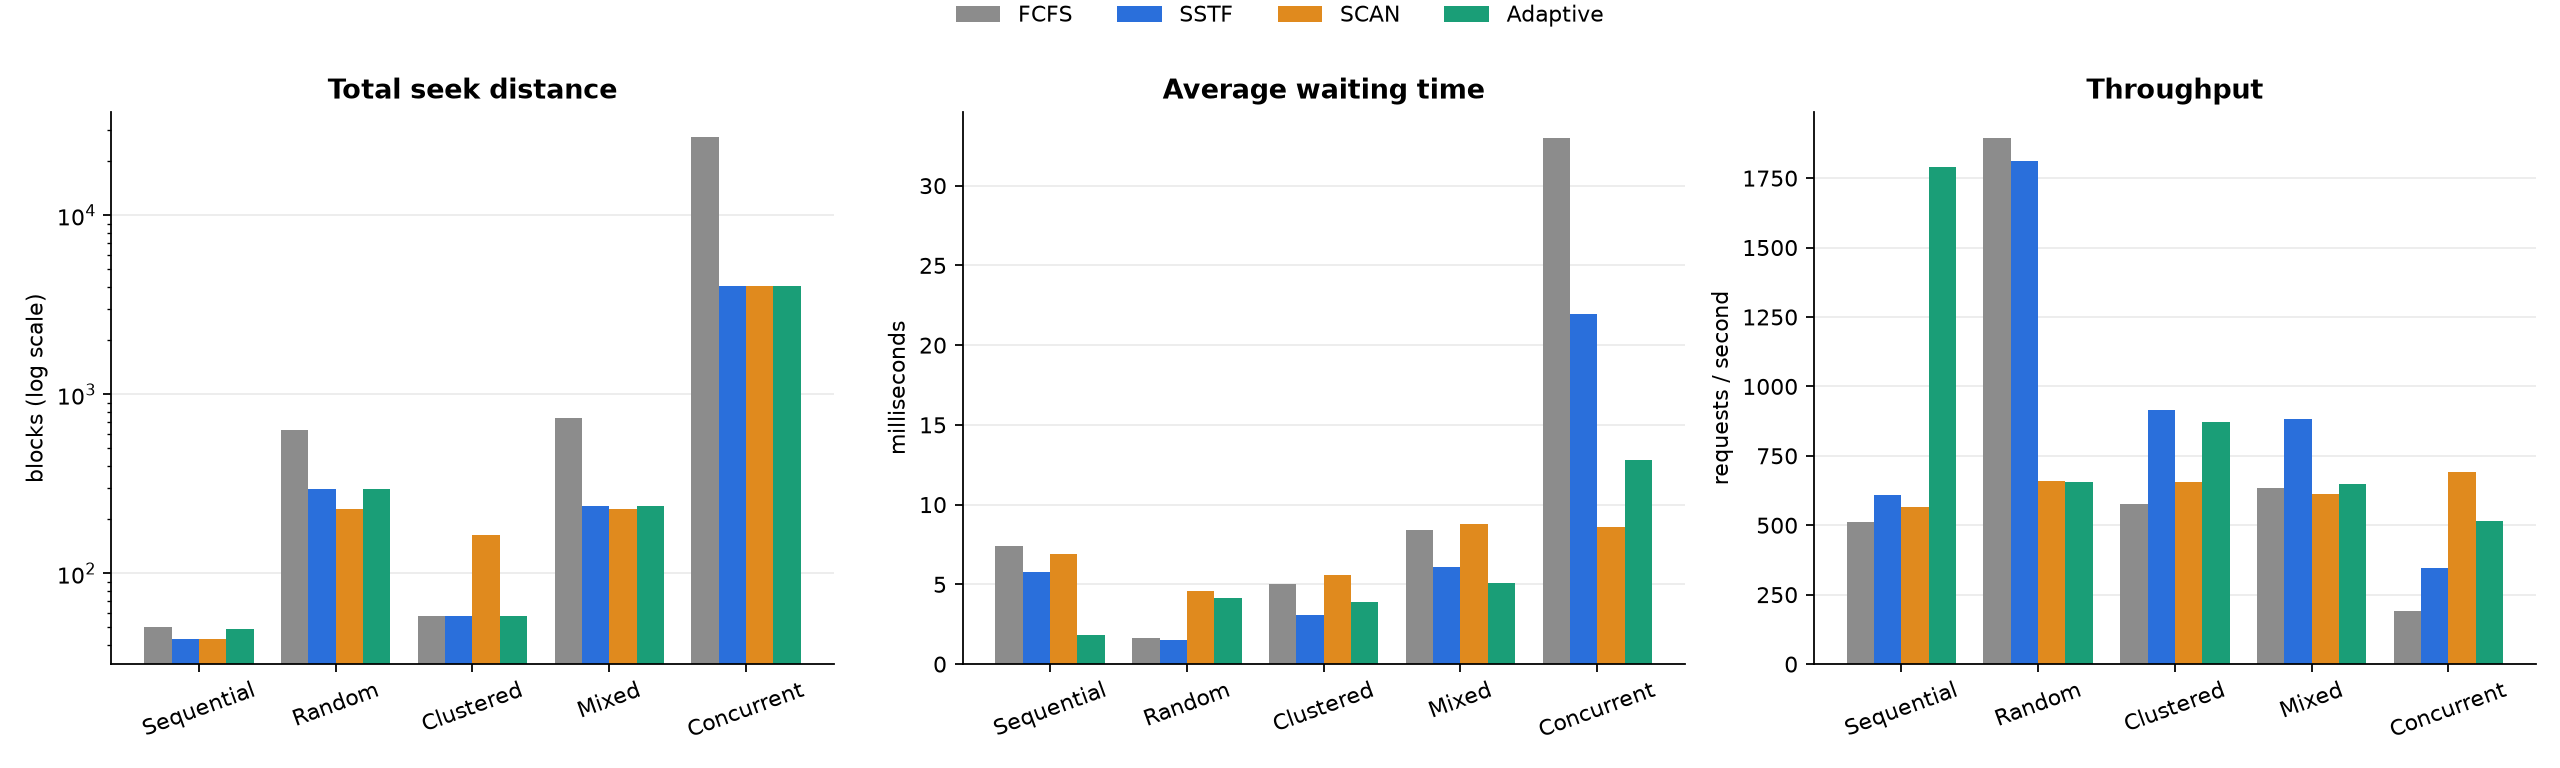
\includegraphics[width=0.9\linewidth]{figures/graphs/summary.png}
\caption[Summary graph from the plotting script (committed CSV)]{Summary graph produced by \code{scripts/plot_results.py} from the repository's committed \code{benchmark.csv}.}
\label{fig:summarypng}
\end{figure}

\noindent \figref{fig:web-bench} and \figref{fig:summarypng} use the repository's committed CSV, recorded on a different machine. Their seek totals for FCFS, SSTF and SCAN equal those in \tabref{tab:bench}, while their timing values and Adaptive totals differ, as discussed under TC24.
% =====================================================================
\clearpage
\section{REFERENCES}
\label{sec:refs}
% =====================================================================
\begingroup
\renewcommand{\section}[2]{}%
\small
\bibliographystyle{IEEEtran}
\bibliography{references}
\endgroup

% =====================================================================
%  APPENDICES (supplementary material after the nine required sections)
% =====================================================================
\clearpage
\appendix
\renewcommand{\thesection}{\Alph{section}}

\section{COMPLIANCE CHECKLIST}
\label{sec:compliance}
The project team has four members, listed on the title page. For a team of four, the university minimums for this report are 8~functional requirements, 4~non-functional requirements, 8~modules, 4~test cases and 1{,}200 qualifying lines of code. \tabref{tab:compliance} shows where each is met.

\begin{table}[H]
\centering
\caption{University requirements and where they are met (team of four)}
\label{tab:compliance}
\small
\begin{tabularx}{\linewidth}{@{}X l l l@{}}
\toprule
\textbf{Requirement} & \textbf{Minimum} & \textbf{Provided} & \textbf{Where} \\
\midrule
Title of the project & --- & yes & Section~\ref{sec:title} \\
Team names and roll numbers & --- & 4 members & Title page \\
Abstract & $\le 250$ words & 230 words & Section~\ref{sec:abstract} \\
Scope narrative & $\le 500$ words & 364 words & Section~\ref{sec:scope} \\
Functional requirements & 8 & 12 & \tabref{tab:fr} \\
Non-functional requirements & 4 & 8 & \tabref{tab:nfr} \\
Modules & 8 & 10 & Section~\ref{sec:modules}, \tabref{tab:modsummary} \\
Tools and technologies & --- & 15 entries & \tabref{tab:tools} \\
Design diagrams and flowcharts & --- & 18 figures (TikZ/PGFPlots) & Section~\ref{sec:design} \\
Figures in the whole report & --- & 39 & List of Figures \\
Qualifying lines of code & 1{,}200 & 2{,}103 & \tabref{tab:locfile}, \tabref{tab:contrib} \\
Lines of code per member & 300 & 408--773 (proposed allocation) & \tabref{tab:contrib} \\
Test cases & 4 & 25 (all passed) & \tabref{tab:tests} \\
Genuine output screenshots & --- & 11 terminal, 6 browser & Sections~\ref{sec:implshots}, \ref{sec:testshots} \\
IEEE references & --- & 22 & Section~\ref{sec:refs} \\
Traceability to the synopsis & --- & modules and FRs mapped & \tabref{tab:synmod}, \tabref{tab:synfr} \\
\bottomrule
\end{tabularx}
\end{table}

\noindent\textbf{Item to complete before submission:} team confirmation of the member-to-module allocation in \tabref{tab:contrib}. The title page, course details and supervisors are taken from the approved synopsis.

\section{SOURCE LISTINGS OF THE SCHEDULING PATH}
\label{app:source}
The three files below form the complete path from a submitted request to the disk: the queue, the scheduler and the dispatcher. They are reproduced in full from the repository.

\lstinputlisting[caption={\code{src/sync/request_queue.c} (complete)},label={lst:full-rq}]{../src/sync/request_queue.c}
\lstinputlisting[caption={\code{src/sched/scheduler.c} (complete)},label={lst:full-sched}]{../src/sched/scheduler.c}
\lstinputlisting[caption={\code{src/storage/virtual_disk.c} (complete)},label={lst:full-vd}]{../src/storage/virtual_disk.c}

\section{REPRODUCING THE RESULTS}
\label{app:repro}
On Ubuntu 22.04 or 24.04 with \code{/dev/fuse} available, the following commands reproduce every result in this report. Run them as a normal user, not as root.

\begin{lstlisting}[style=shstyle,caption={Commands used to produce the results},label={lst:repro}]
sudo apt install -y build-essential pkg-config libfuse3-dev fuse3 \
                    python3-pandas python3-matplotlib
git clone https://github.com/Sharmaditya2k05/FUSE.git && cd FUSE
make                                   # Figure: build
./mkfs.schedfs disk.img 16M            # TC04
mkdir -p mnt && ./schedfs disk.img mnt --sched=sstf
echo 'Operating Systems' > mnt/demo.txt && cat mnt/demo.txt
fusermount3 -u mnt && cat filesystem.log
make test                              # TC01-TC03, TC19, TC21, TC22
./schedfs-bench --all                  # TC24, writes benchmark.csv
python3 scripts/plot_results.py        # graphs in results/
\end{lstlisting}

\end{document}
